%% Manuscript: Automated Characterization of PDs and RDA
%% Using iopjournal class

\documentclass{iopjournal}

\usepackage{graphicx}
\usepackage{booktabs}
\usepackage{amsmath}
\usepackage{amssymb}
\usepackage{xcolor}
\usepackage{hyperref}

\begin{document}

\articletype{Paper}

\title{GROND: Automated Characterization of Periodic and Rhythmic EEG Patterns}

\author{Jin~Jing$^{1,\dagger}$, ChenXi~Sun$^{1,2,\dagger}$, Tianyu~Zhang$^{1}$, Matthew~Byrd$^{1}$, Alexandra-Maria~T\u{a}u\c{t}an$^{3}$, Lara~Basovic$^{3}$, Peter~N~Hadar$^{3}$, Marta~P~Fernandes$^{3}$, Daniel~Goldenholz$^{1}$, Jennifer~Kim$^{4}$, Aaron~F~Struck$^{5}$, Sahar~F~Zafar$^{3,\ddagger}$, M~Brandon~Westover$^{1,2,\ddagger,*}$}

\affil{$^1$Department of Neurology, Clinical Data Animation Center, Beth Israel Deaconess Medical Center/Harvard Medical School, Boston, MA, USA}

\affil{$^2$Stanford University, Palo Alto, CA, USA}

\affil{$^3$Department of Neurology, Massachusetts General Hospital/Harvard Medical School, Boston, MA, USA}

\affil{$^4$Department of Neurology, Yale University School of Medicine, New Haven, CT, USA}

\affil{$^5$Department of Neurology, Washington University in St.~Louis, St.~Louis, MO, USA}

\affil{$^\dagger$These authors contributed equally as co-first authors.}

\affil{$^\ddagger$These authors contributed equally as co-senior authors.}

\affil{$^*$Author to whom any correspondence should be addressed.}

\email{mbwest@stanford.edu}

\keywords{EEG, periodic discharges, rhythmic delta activity, deep learning, signal processing}

\begin{abstract}
\textbf{Objective.} Periodic discharges (PDs) and rhythmic delta activity (RDA) are common electroencephalographic (EEG) patterns in critically ill patients that require detailed characterization---including lateralization, spatial localization, discharge timing, and frequency estimation---according to the American Clinical Neurophysiology Society (ACNS) 2021 standardized terminology. Manual characterization is subjective, time-consuming, and exhibits substantial inter-rater variability. This study presents a comprehensive automated system for characterizing all four major subtypes: lateralized periodic discharges (LPD), generalized periodic discharges (GPD), lateralized rhythmic delta activity (LRDA), and generalized rhythmic delta activity (GRDA).

\textbf{Approach.} Two complementary pipelines were developed: the PD-Profiler and the RDA-Profiler. The PD-Profiler combines a per-channel convolutional neural network (ChannelPD-Net) with hemisphere-specific learned evidence traces (HemiCET-UNet), dynamic programming with an approximately-periodic prior, and discharge-locked topographic localization. The RDA-Profiler uses iterative narrowband Hilbert refinement (NB-Hilbert) for frequency and lateralization, with phase-locking value (PLV) analysis for spatial extent. Both pipelines were trained and evaluated on 12,238 EEG segments from 11,578 unique patients, annotated by four expert electroencephalographers through iterative human-in-the-loop label refinement.

\textbf{Main results.} Three electroencephalographers not involved in algorithm development (SZ, TZ, AS) and the primary annotator (MW) independently scored 200 stratified segments per pattern subtype, with analysis restricted to segments accepted by a majority of the four raters. On every frequency and laterality task, the algorithm matched or exceeded expert--expert (EE) inter-rater agreement: it \emph{exceeded} the EE intraclass correlation coefficient (ICC) on LPD frequency (mean expert--algorithm ICC 0.931 vs.\ EE 0.897; paired segment-bootstrap $\Delta=+0.034$, 95\% confidence interval (CI) $[+0.016, +0.055]$, $p<0.001$), and was statistically indistinguishable from EE on GPD frequency, GRDA frequency, LRDA frequency, LPD laterality, and LRDA laterality (per-pair ICCs, $\Delta$'s, and $p$-values in figure~\ref{fig:irr_main} and \S\ref{sec:reeval}). PD discharge timing achieved an F1 of 0.889 at single-sample precision (1.0~ms median timing error at 200~Hz). Pattern lateralization area under the receiver operating characteristic curve (AUC) was 0.989 for PD hemisphere ($n = 1{,}274$), 0.911 for LPD vs.\ GPD ($n = 7{,}037$), and 0.837 for RDA ($n = 4{,}253$). PD spatial localization reached 97.3\% of expert inter-rater Jaccard agreement; RDA spatial extent matched expert--expert ICC (0.371 vs.\ 0.373), at the ceiling imposed by the inherent noise of verbal region-counting labels (see Discussion).

\textbf{Significance.} This work presents the first system to jointly characterize lateralization, spatial localization, discharge timing, and frequency for both periodic and rhythmic EEG patterns, achieving algorithm--expert agreement at the level of expert--expert agreement across all tasks. In post-hoc review of discordant cases, experts judged the algorithm's frequency estimates more accurate than the original expert labels in 94\% of cases. Automated characterization can now both substitute for and improve manual annotation in critical-care EEG.
\end{abstract}

%%%%%%%%%%%%%%%%%%%%%%%%%%%%%%%%%%%%%%%%%%%%%%%%%%
\section{Introduction}
\label{sec:introduction}

Continuous EEG (cEEG) monitoring is widely used across acute-care settings---including neurological, medical, and surgical intensive care units (ICUs), emergency departments, and step-down units---for detecting seizures and identifying patterns associated with secondary brain injury in critically ill patients~\cite{claassen2004,zafar2020}. Among the most clinically significant findings are periodic discharges (PDs) and rhythmic delta activity (RDA), which lie along the ictal--interictal continuum and are associated with increased risk of seizures, neuronal injury, and poor outcomes~\cite{chong2005,rodriguez2017,vespa2016,struck2016,tao2020,parikh2023}. The ACNS standardized critical care EEG terminology, revised in 2021, provides a framework for describing these patterns along multiple dimensions: main term (periodic vs.\ rhythmic), lateralization (lateralized vs.\ generalized vs.\ bilateral independent), spatial distribution (e.g., frontal predominant, hemispheric), and quantitative features including repetition frequency and regularity~\cite{hirsch2021}.

A growing body of evidence indicates that periodic and rhythmic patterns are not merely markers of underlying brain injury but can themselves contribute to neuronal damage. Microdialysis and FDG-PET studies have shown that periodic discharges, like seizures, are accompanied by metabolic crisis and elevated glucose utilization in injured cortex~\cite{vespa2016,struck2016}, providing direct biological evidence that these patterns impose a metabolic burden on vulnerable tissue. At the population level, our group has shown that the proportion of monitoring time a patient spends with periodic or rhythmic epileptiform activity is independently associated with worse discharge neurological outcomes. In an analysis of 11.02~TB of cEEG from 1{,}967 critically ill patients, peak epileptiform-activity burden was independently associated with poor discharge modified Rankin Scale score ($p<10^{-4}$); after adjustment for age, illness severity, and other clinical covariates, increasing peak burden from 0\% to 100\% of monitoring time raised the estimated probability of a poor outcome by approximately 35\%~\cite{zafar2021}. A subsequent counterfactual matching analysis incorporating pharmacokinetic--pharmacodynamic modeling of antiseizure-medication exposure produced concordant results: untreated patients with maximum epileptiform-activity burden of $\geq 75\%$ had an estimated 22 percentage-point increase in the probability of a poor outcome relative to patients with $<25\%$ burden, and even moderate but long-lasting burden ($2$--$10\%$ of monitoring time) increased the probability of a poor outcome by an estimated 13.5 percentage points~\cite{parikh2023}. Together these observations are consistent with a dose-response, and plausibly causal, contribution of periodic and rhythmic epileptiform activity to neurological injury.

Time-burden alone, however, is a coarse summary of what is fundamentally a multidimensional phenomenon. Both theoretical considerations and prior experimental work suggest that, beyond \emph{whether} a patient is in an epileptiform state, the \emph{characteristics} of that state matter: faster discharge frequencies and broader spatial involvement plausibly impose greater metabolic demand and a greater cumulative dose of synchronous neuronal activity on vulnerable cortex~\cite{vespa2016,struck2016,claassen2004,gaspard2013}. Until now, however, we have not had automated tools that can reliably quantify these features---frequency, spatial localization, lateralization, and individual discharge timing---at the data scales required for population-level studies. Building such tools is the principal motivation for the present work: only when these characteristics can be measured reproducibly and at scale will it become possible to study \emph{how}, not merely \emph{whether}, periodic and rhythmic epileptiform patterns predict and contribute to adverse neurological outcomes.

Despite the standardization of terminology, manual characterization of PDs and RDA remains subjective and labor-intensive. A trained electroencephalographer must identify the pattern type, determine its spatial distribution across the scalp, estimate its repetition frequency, and describe its temporal evolution---all from visual inspection of multi-channel EEG tracings. Inter-rater reliability for these characterization tasks varies widely: lateralization (generalized vs.\ lateralized) shows moderate to good agreement, while spatial extent and frequency estimation exhibit substantially lower reliability~\cite{gaspard2014,leitinger2015,jing2023irr}. The clinical similarity of LRDA to lateralized periodic discharges further complicates pattern classification at the boundary between rhythmic and periodic phenomena~\cite{gaspard2013}. The need for expert review creates bottlenecks in clinical workflow, particularly during overnight monitoring when specialist coverage is limited.

Prior automated systems have addressed pattern detection and classification but not the full characterization problem. Early signal-processing systems such as the ACNS-based detector of F\"urbass et al.~\cite{furbass2015} and the NeuroTrend platform~\cite{herta2015} demonstrated feasibility of automated pattern recognition in critical care EEG; McGraw et al.~\cite{mcgraw2024} introduced a method for automated quantification of periodic discharge bursts. The IIIC (Interictal--Ictal-Injury Continuum) dataset introduced by Jing et al.~\cite{jing2023} provides expert consensus labels for pattern classification (LPD, GPD, LRDA, GRDA, seizure, other) based on crowd-sourced annotations from 10 or more expert raters per segment, and deep learning models trained on this dataset---and on related datasets of epileptiform discharges~\cite{jing2020}---achieve high classification accuracy for distinguishing among pattern types~\cite{ge2023,zheng2022}. None of these systems, however, addresses lateralization, spatial localization, individual discharge timing, and frequency simultaneously. The closest prior attempt is T\u{a}u\c{t}an et al.~\cite{tautan2025}, which recently described a signal-processing approach to joint frequency and spatial-extent estimation using autocorrelation and spectral analysis; that work demonstrated the feasibility of automated characterization but reported Spearman frequency correlations below 0.25 for all subtypes and limited agreement with expert spatial-extent annotations.

To address these needs, we present GROND (Generalized Rhythmic and Oscillatory Neurophysiology Descriptor), an automated system for comprehensive characterization of periodic discharges and rhythmic delta activity in continuous EEG. Given a 10-second EEG segment containing a periodic or rhythmic pattern, GROND automatically determines (1) lateralization (left, right, or bilateral/generalized), (2) spatial localization (which brain regions are involved), (3) frequency of the periodic or rhythmic pattern, (4) for PDs, the precise timing of each individual discharge, and (5) for PDs, whether the pattern represents bilateral independent periodic discharges (BIPD). GROND produces a structured verbal description following ACNS 2021 nomenclature (e.g., ``LPD, left-sided, at 1.5~Hz, left frontotemporal predominant'').

This work makes four contributions. First, we present a modular pipeline architecture that combines learned neural evidence (convolutional neural networks) with structured temporal inference (dynamic programming) for PD characterization, and iterative narrowband signal processing for RDA characterization. Second, we introduce discharge-locked topographic localization---a novel spatial-localization method that computes the mean voltage topography at the moment of each detected discharge, bypassing the subjective channel-counting approach used in prior work. Third, we describe a systematic ``contest of methods'' framework in which 76 algorithm variants were compared for RDA characterization and over 30 variants for PD spatial localization, providing empirical evidence for design decisions. Fourth, we benchmark all results against multi-rater expert annotations with quantitative inter-rater reliability analysis, enabling direct comparison of algorithm--expert agreement with expert--expert agreement across all characterization tasks.

%%%%%%%%%%%%%%%%%%%%%%%%%%%%%%%%%%%%%%%%%%%%%%%%%%
\section{Methods}
\label{sec:methods}

\subsection{Dataset and Annotations}
\label{sec:dataset}

\subsubsection{Ethics statement.}

This study was conducted under protocols approved by the institutional review boards of Massachusetts General Hospital (protocols \#2023P000487 and \#2024P002630) and Beth Israel Deaconess Medical Center (protocols \#2022P000481 and \#2022P000417). Both review boards waived the requirement for informed consent for this retrospective analysis of de-identified EEG recordings.

\subsubsection{EEG Data.}

We drew 12,238 non-excluded EEG segments from three sources (table~\ref{tab:dataset}). Each segment consisted of 10 seconds of 19-channel monopolar EEG recorded at 200~Hz in common average reference montage (2,000 samples per channel). Segments were classified into four subtypes based on the dominant pattern: LPD ($n = 4{,}170$), GPD ($n = 3{,}337$), LRDA ($n = 1{,}408$), and GRDA ($n = 3{,}323$). An additional 990 segments were excluded during quality review. Representative examples of each pattern type, including both clear and ambiguous cases, are shown in figure~\ref{fig:eeg_examples}.

The first data source consisted of segments from the IIIC dataset~\cite{jing2023}, comprising 10-minute recordings from which the center 10-second segment (the labeled epoch) was extracted. Each of these segments had pattern classification votes from 10 or more expert electroencephalographers (3,529 segments: 1,846 LPD, 1,024 GPD, 239 LRDA, 420 GRDA). The second source consisted of segments selected from pattern-specific clinical EEG databases and classified by a single expert rater (MW). The third source was a 38-patient expert dataset annotated independently by four raters (LB, PH, SZ, MW) for pattern classification, frequency, spatial extent, and discharge timing.

\begin{table}[t]
\caption{Dataset statistics. The ``Unique patients'' total (11,578) is the deduplicated count across all four subtypes; only one patient contributed segments to more than one subtype, so the total is essentially the column sum. Verified by computing the union of patient identifiers across the LPD, GPD, LRDA, and GRDA cohorts in \texttt{segment\_labels.csv}: a single patient (anonymous identifier \texttt{abn1762}) appeared in two cohorts (LPD and GRDA), and no patient appeared in three or more.}
\centering
\begin{tabular}{l r r r r r}
\hline
 & LPD & GPD & LRDA & GRDA & Total \\
\hline
Segments (non-excluded) & 4,170 & 3,337 & 1,408 & 3,323 & 12,238 \\
Unique patients & 3,953 & 3,086 & 1,381 & 3,159 & 11,578 \\
Expert-reviewed frequency & 1,499 & 1,539 & 654 & 1,381 & 5,073 \\
Discharge/wave timing & 917 & 1,036 & 189 & 313 & 2,159/502 \\
Spatial annotations & 352 & 260 & 29 & 177 & 818 \\
IIIC crowd votes ($\geq$10 raters) & 1,846 & 1,024 & 239 & 420 & 3,529 \\
\hline
\end{tabular}
\label{tab:dataset}
\end{table}

\subsubsection{Annotation Framework.}

We developed a multi-layer annotation framework with task-specific interactive review tools.

\textbf{Pattern classification and laterality.} For IIIC crowd-labeled segments, pattern subtype was assigned based on the majority vote across expert raters. For MW-labeled segments, classification was performed during visual review. Dedicated review using a symmetric channel-layout viewer yielded laterality annotations (left vs.\ right hemisphere dominance) for 1,336 LPD segments and 1,039 LRDA segments. We reviewed 1,374 LRDA segments across three batches and rejected 338 as not meeting LRDA criteria; the rejected segments were excluded from subsequent analysis.

\textbf{Frequency.} Expert raters reviewed frequency labels for 5,073 segments across all four subtypes. For PD subtypes, MW annotated frequency during combined timing--frequency--laterality review. For RDA subtypes, MW reviewed frequency using an interactive viewer that displayed the NB-Hilbert algorithm estimate as a default value, with a narrowband-filtered overlay for visual confirmation. The reviewer could accept the default, type any other frequency judged correct, or reject the segment; MW reviewed 993 RDA segments, yielding 399 frequency corrections and 594 confirmations. We added 453 LRDA/GRDA frequency labels from segments with at least 50\% IIIC crowd agreement. Three additional expert raters (LB, PH, SZ) independently annotated frequency for 1,060 segments ($\sim$265 per subtype) from the expert dataset.

\textbf{Discharge timing.} An expert (MW) annotated individual discharge times for 1,953 PD segments (917 LPD, 1,036 GPD) through three rounds of iterative model-assisted review. In the first round, MW annotated discharge times de novo. In subsequent rounds, the HemiCET-UNet + dynamic programming (DP) algorithm generated candidate discharge times that MW reviewed and corrected, yielding 61 corrected discharge sequences and 15 rejected segments across three review cycles.

\textbf{Annotation strategy and rater coverage.} MW labeled the full corpus using the interactive narrowband-overlay tools developed for the present work; SZ, AS, and TZ each independently labeled a more limited subset (described below). We report two complementary inter-rater evaluations:

\textbf{(i) Canonical 4-rater independent-expert evaluation (MW, SZ, TZ, AS).} Three co-author electroencephalographers (SZ, TZ, and AS) -- none of whom contributed to algorithm development -- independently scored lateralization, frequency, and discharge timing on the same 200 stratified segments per pattern subtype (LPD, GPD, LRDA, GRDA; figure~\ref{fig:indep_expert_freq}). Each rater also recorded a per-segment accept/reject decision (rejected segments were judged by the rater not to be valid instances of the labeled subtype). The canonical inter-rater reliability (IRR) analysis includes only segments where the per-segment accept count exceeded the per-segment reject count (i.e.\ a strict majority across the four raters), removing dataset-labeling noise from the IRR computation; an individual rater's labels are used only on segments where that rater also accepted the segment. Under this canonical inclusion rule, segment counts per task are LPD~177/200, GPD~191/200, LRDA~104/200, and GRDA~134/200; rejection rates differed by rater (MW~0--13\%, SZ~5--44\%, TZ~7--35\%, AS~15--73\%) with the highest rates on LRDA. Inter-rater reliability across all $\binom{4}{2}=6$ expert--expert pairs and all 4 expert--algorithm pairs is reported in figure~\ref{fig:irr_main} (paired EE vs.\ EA bars with bootstrap 95\% CIs and significance tests) and in detail in the supplementary analysis document (\texttt{paper\_materials/independent\_expert\_tasks/analysis\_v1.md}).

\textbf{(ii) Independent prior-cohort evaluation (PH, LB, SZ, MW; Tautan et al.~\cite{tautan2025} dataset).} As a check on a different annotation cohort, we additionally evaluated against the three expert raters (PH, LB, SZ) who labeled the Tautan et al.\ dataset, with MW added as a fourth rater on the same segments. These labels were produced without the interactive narrowband-overlay tools described above and are therefore noisier than the canonical cohort by construction; the cohort's expert--expert ICCs (LPD~0.50, GPD~0.47, LRDA~0.64, GRDA~0.84) reflect this. The algorithm's agreement with these four raters is reported in table~\ref{tab:phlbsz_cohort}.

\textbf{Spatial extent and channel involvement.} Three expert raters (LB, PH, SZ) annotated per-channel spatial involvement for 818 segments (352 LPD, 260 GPD, 29 LRDA, 177 GRDA) using an interactive topoplot viewer with per-channel toggling. An additional 1,980 IIIC segments received MW spatial extent annotations. Region-level spatial descriptions followed the 16-region parcellation from the morgoth-viewer module, which includes transitional zones (frontotemporal, centro-parietal, fronto-central, parieto-occipital) compatible with ACNS 2021 nomenclature.

\subsubsection{Evaluation Framework.}

All evaluations used patient-stratified cross-validation to ensure no patient appeared in both training and evaluation sets. For models trained with $k$-fold cross-validation (ChannelPD-Net, HemiCET-UNet), 5-fold patient-stratified splits were used, and evaluation was performed on the held-out fold for each patient. For methods not requiring training (NB-Hilbert, RDA-PLV), leave-one-patient-out (LOPO) cross-validation was not applicable, and all available labeled segments were used for evaluation.

We evaluated frequency estimation using quality-filtered labels to reduce the influence of annotation noise. A segment qualified for quality-filtered evaluation if any of the following criteria were met: (1) MW reviewed the frequency, (2) all three expert raters (LB, PH, SZ) provided independent labels, or (3) at least 10 IIIC crowd votes with at least 80\% pattern agreement were available. For multi-rater segments, we defined expert frequency as the mean across available raters.

To enable direct comparison with prior work, we quantified inter-rater reliability using the intraclass correlation coefficient (ICC(3,1)) of Shrout and Fleiss~\cite{shrout1979} and percentage agreement, following the framework of T\u{a}u\c{t}an et al.~\cite{tautan2025}. We treated the algorithm as an additional rater in the ICC computation, enabling direct comparison of algorithm--expert agreement with expert--expert agreement.

\subsubsection{Contest-of-methods development strategy.}
\label{sec:contest_strategy}

The PD-Profiler and RDA-Profiler were each developed through a systematic ``contest of methods'' in which a wide variety of candidate algorithms was implemented and compared empirically before any single approach was selected for the production pipeline. Across all subtasks (PD frequency estimation, PD spatial localization, PD discharge timing, RDA lateralization, and RDA frequency estimation), more than 300 distinct method variants were implemented and evaluated. PD frequency estimation alone progressed through nine refinement rounds comprising 192 experiments, spanning autocorrelation, fast Fourier transform (FFT), peak counting, Teager--Kaiser energy, harmonic product spectrum, matched filters, multi-montage estimators, ridge regression on log-frequency targets, and CNN-based approaches. PD spatial localization was selected from 26 contest entries spanning amplitude-based, phase-coherence-based, and CNN-probability-based methods. The RDA lateralization contest evaluated 76 algorithm variants on 4,253 segments, and a separate GPD-specific frequency contest compared 25 variants. After identifying each subtask's best-performing approach in isolation, we combined the winning components and refined the integrated pipeline. Throughout the Results section, contest entries are referenced by short codes whose letter prefixes indicate the contest cohort: \textbf{L} = single-pass laterality variants (e.g., L24); \textbf{V} = variance- or PLV-based channel-selection variants (e.g., V04, V05); \textbf{W} = two-pass iterative narrowband refinement variants (e.g., W05, the overall RDA winner, renamed NB-Hilbert in the main text); and \textbf{C} = discrete configurations of the discharge-timing pipeline. Appendix~\ref{app:contest} documents the full naming convention and references the complete contest logs. This empirical, contest-driven development was essential because no single signal-processing or machine-learning paradigm proved best for all subtasks, and several methods that performed well in isolation degraded when naively combined with others. The contest is a descriptive method-selection procedure, not a formal hypothesis test: we report contest entries' point estimates so readers can see which design choices mattered, but we do not assign p-values across the 300+ variants, and the ranking among close competitors is not itself the claim. The claim about the production algorithm's performance is supported separately by the prospective independent-expert evaluation (\S\ref{sec:reeval}, figure~\ref{fig:irr_main}), in which the production system is scored against four expert raters who did not participate in algorithm development.

\begin{figure}[htbp]
\centering
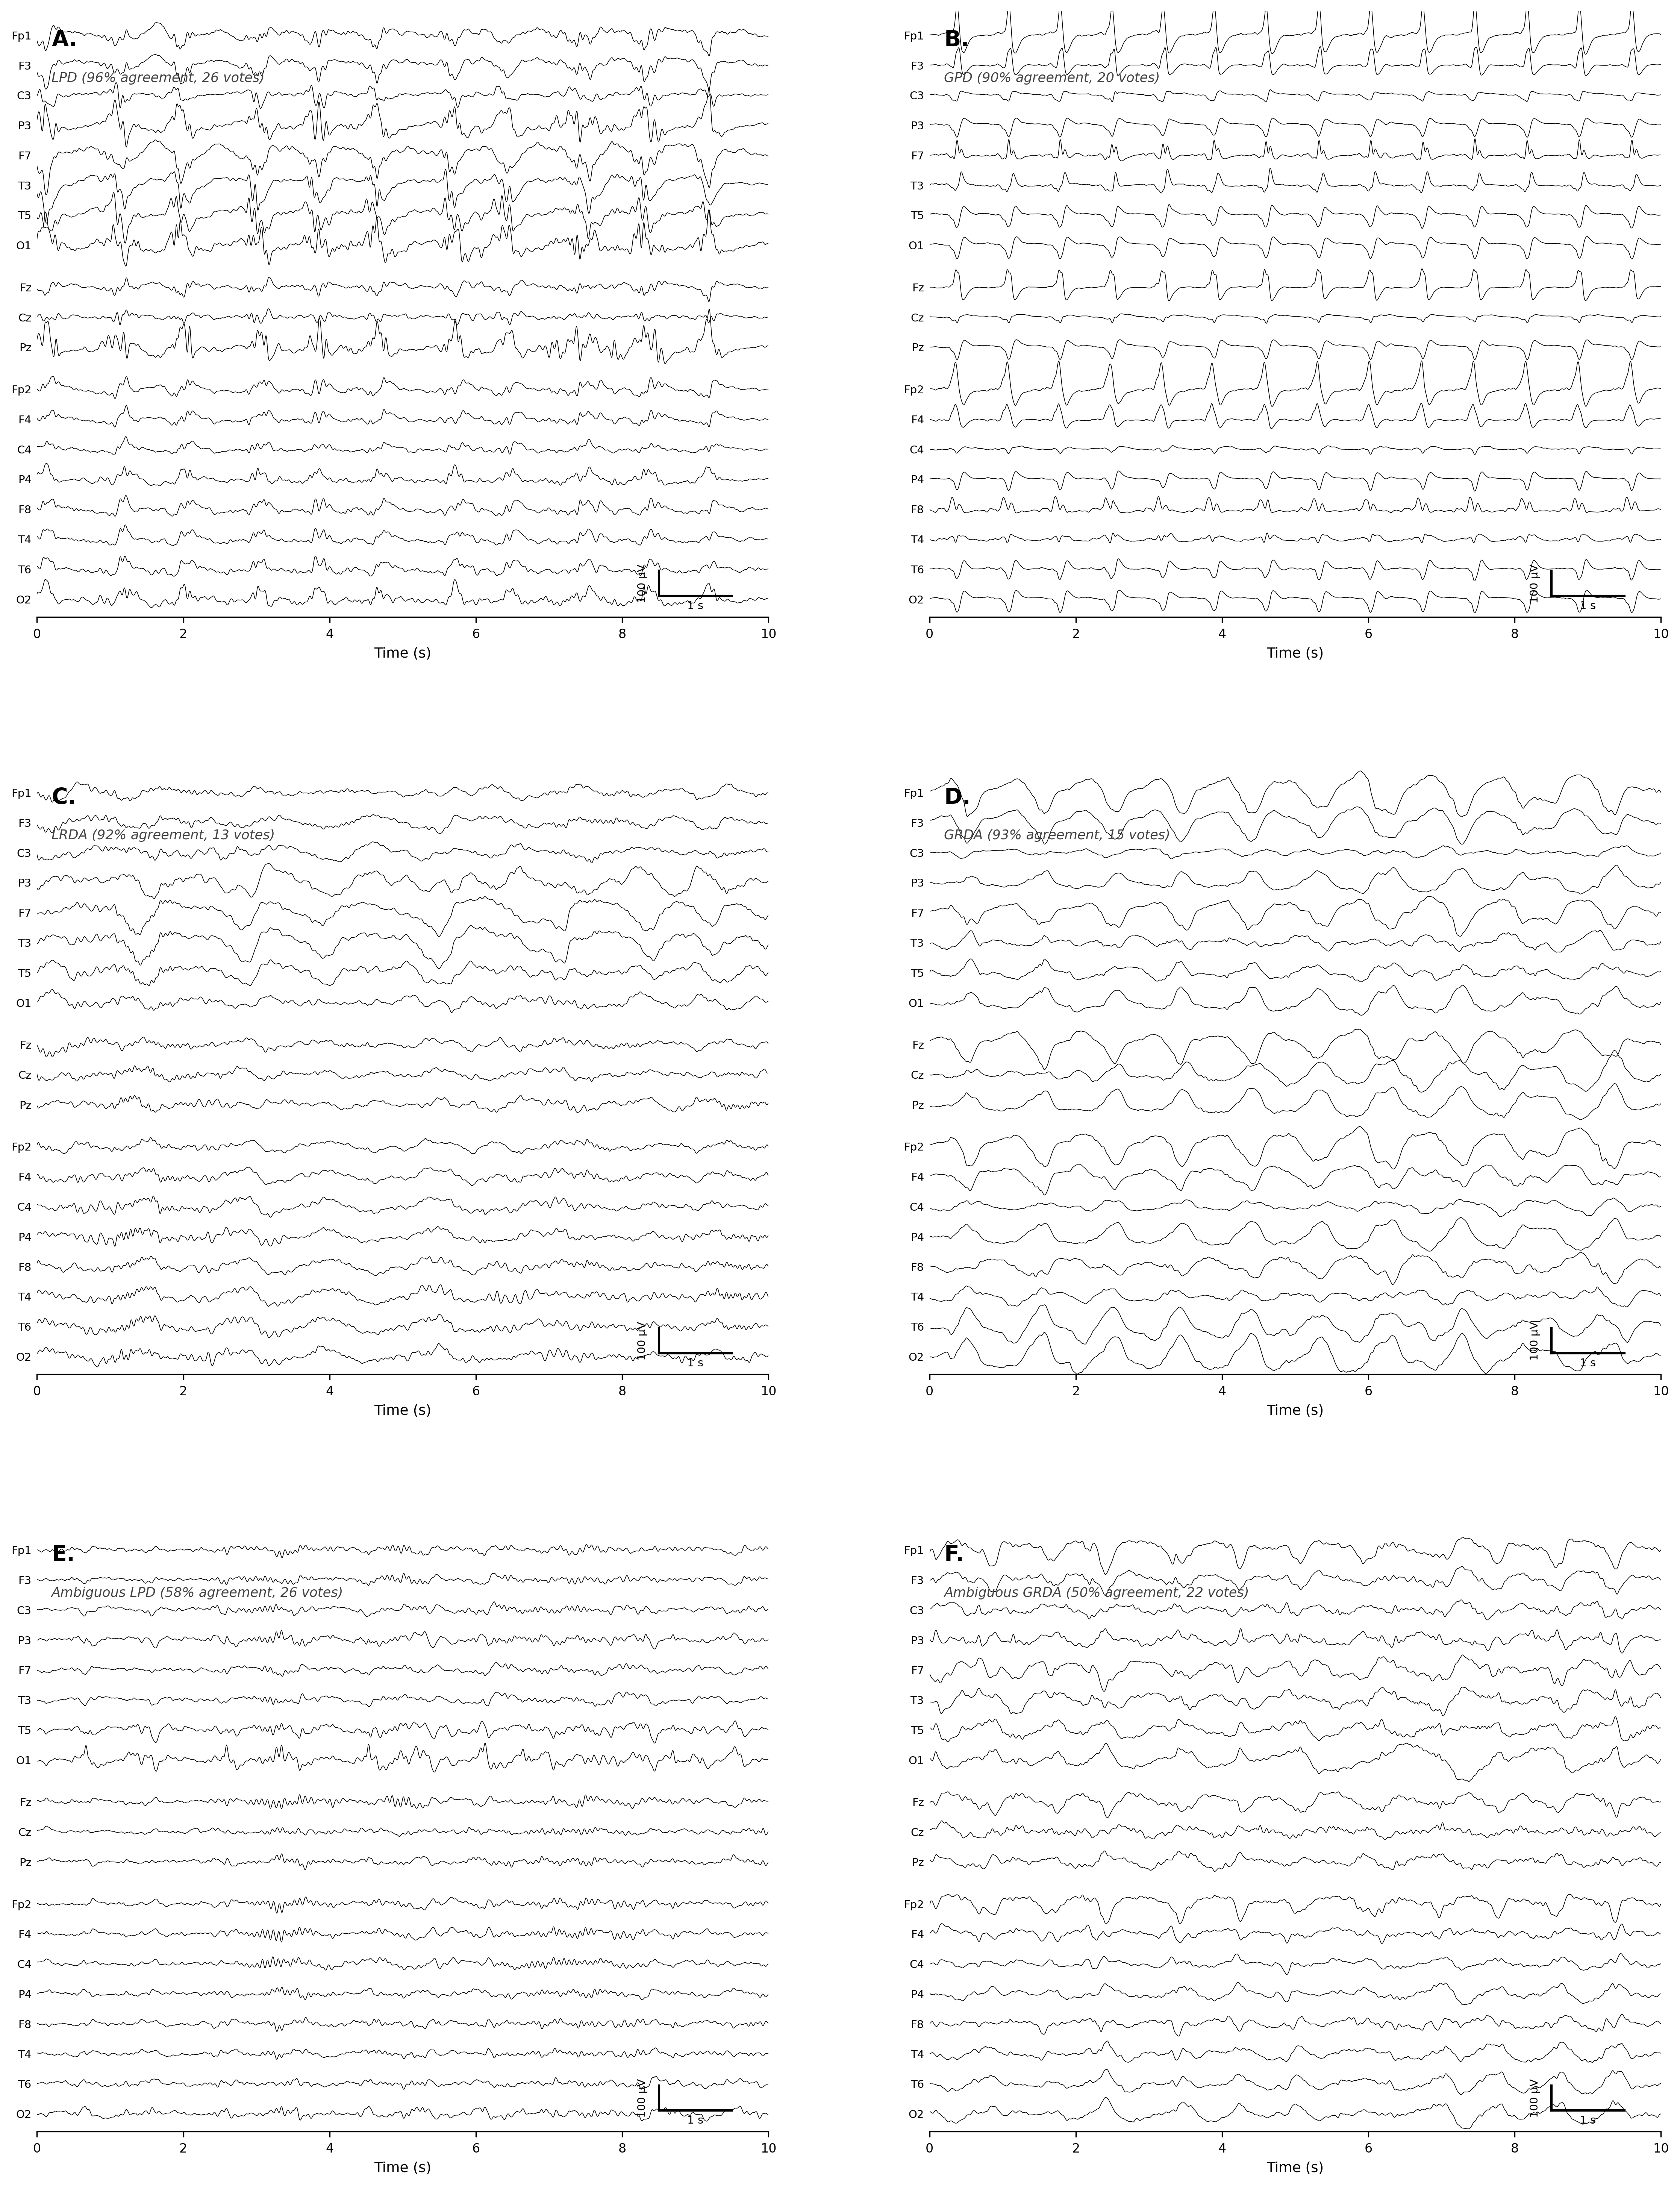
\includegraphics[width=\textwidth]{figures/fig1_eeg_examples.png}
\caption{Representative EEG examples of periodic and rhythmic patterns. Six 10-second EEG segments displayed in average-reference montage (19 channels, 200~Hz, bandpass 0.5--20~Hz). Channels are grouped by hemisphere: left parasagittal (Fp1, F3, C3, P3), left temporal (F7, T3, T5, O1), midline (Fz, Cz, Pz), right parasagittal (Fp2, F4, C4, P4), and right temporal (F8, T4, T6, O2). \textbf{(A)}~Clear lateralized periodic discharges (LPD). \textbf{(B)}~Clear generalized periodic discharges (GPD). \textbf{(C)}~Clear lateralized rhythmic delta activity (LRDA). \textbf{(D)}~Clear generalized rhythmic delta activity (GRDA). \textbf{(E)}~Ambiguous LPD case with lower inter-rater agreement. \textbf{(F)}~Ambiguous GRDA case with lower inter-rater agreement. Clear cases (A--D) were selected from segments with at least 80\% agreement among at least 10 IIIC expert raters; ambiguous cases (E--F) have lower agreement, illustrating the challenge of pattern classification. Scale bar: 100~$\mu$V.}
\label{fig:eeg_examples}
\end{figure}

\subsection{PD Characterization Pipeline (PD-Profiler)}
\label{sec:pd_pipeline}

The PD characterization pipeline, hereafter referred to as the PD-Profiler (figure~\ref{fig:pd_pipeline}), processed 19-channel monopolar EEG segments in a single forward pass, producing lateralization, spatial localization, discharge timing, frequency estimation, and a structured verbal description. The pipeline comprised five components operating on a shared 18-channel bipolar representation derived from the monopolar input using standard longitudinal and transverse bipolar pairs.

\begin{figure}[htbp]
\centering
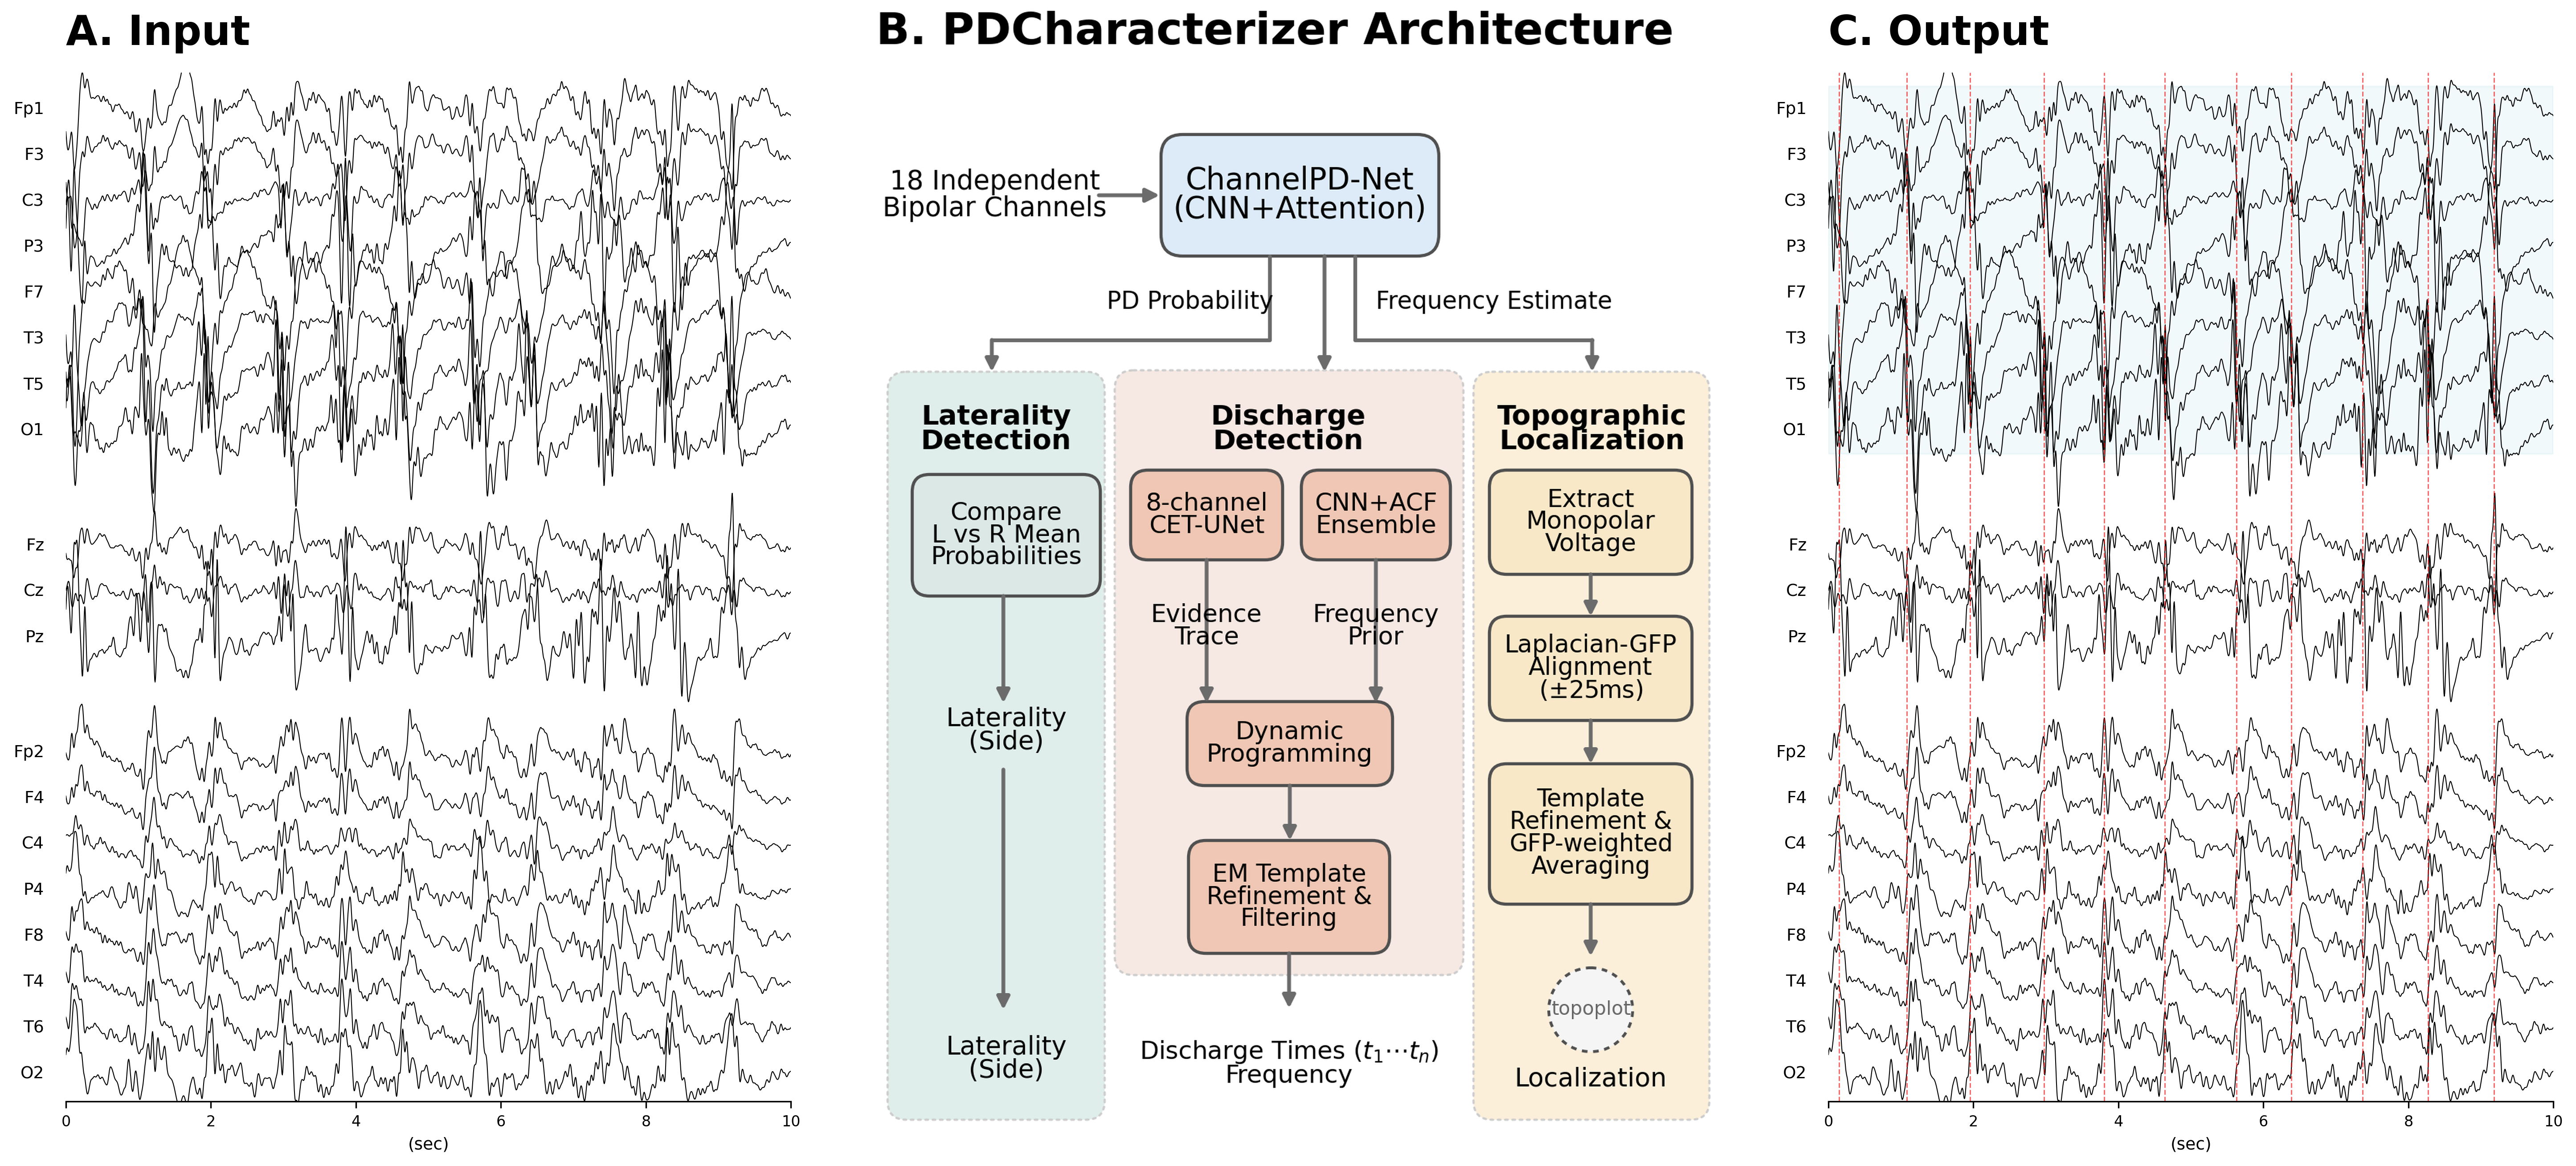
\includegraphics[width=\textwidth]{figures/fig2_pd_pipeline.png}
\caption{The PD-Profiler combines neural evidence with structured dynamic-programming inference to characterize PDs. Three-panel overview of the periodic discharge (PD) characterization pipeline applied to an example LPD segment. \textbf{(A)}~Input: raw 19-channel average-reference EEG (10 seconds, 200~Hz). \textbf{(B)}~Pipeline architecture: 18 independent bipolar channels are processed by ChannelPD-Net (CNN+Attention), which produces per-channel PD probabilities and frequency estimates. Three downstream modules operate in parallel: (1)~Laterality Detection compares left versus right hemisphere mean probabilities; (2)~Discharge Detection uses 8-channel HemiCET-UNet evidence and CNN+ACF frequency prior fed into dynamic programming with expectation-maximization (EM) template refinement, yielding individual discharge times and inter-peak-interval (IPI) derived frequency; (3)~Topographic Localization extracts monopolar voltage at discharge peaks, applies Laplacian--global field power (GFP) alignment with two-pass template refinement and GFP-squared-weighted averaging to produce a spatial localization map. \textbf{(C)}~Output: the same EEG with red dashed lines marking detected discharge times, light blue shading on the involved hemisphere, a Laplacian topoplot showing the discharge topography, and a verbal description following ACNS 2021 standardized nomenclature. Scale bar: 100~$\mu$V.}
\label{fig:pd_pipeline}
\end{figure}

\begin{table}[t]
\caption{PD-Profiler components.}
\centering
\begin{tabular}{l l r l}
\hline
Component & Architecture & Parameters & Role \\
\hline
ChannelPD-Net & CNN + Attention & ${\sim}$50K & Per-channel PD detection and frequency \\
HemiCET-UNet & Encoder--decoder U-Net & ${\sim}$525K & Frame-level discharge evidence \\
HPP & Pointiness + Teager--Kaiser energy operator (TKEO) & -- & Handcrafted Peak Prior evidence \\
Dynamic Programming & Viterbi-style DP & -- & Temporal inference with periodic prior \\
CNN+ACF Ensemble & ChannelPD-Net + ACF & -- & Frequency prior for DP \\
Hybrid-PLV & Phase-locking value & -- & Spatial localization (channel scoring) \\
Discharge-locked topo & Laplacian--GFP alignment & -- & Topographic localization \\
\hline
\end{tabular}
\label{tab:pd_components}
\end{table}

\subsubsection{ChannelPD-Net.}

ChannelPD-Net was a lightweight one-dimensional convolutional neural network (CNN) with temporal attention pooling that operated independently on each of 18 bipolar EEG channels. Given a single 10-second z-scored channel (2,000 samples at 200~Hz), the model jointly predicted (i) the probability that a periodic discharge pattern was present and (ii) the log-frequency of the pattern. The architecture comprised four convolutional blocks (kernel sizes 51, 25, 13, 7; channels 16, 32, 64, 64; stride 2 throughout) with batch normalization, Gaussian Error Linear Unit (GELU) activation, and dropout (0.1--0.2), downsampling the temporal dimension by a factor of 16 to 125 time steps. A learned temporal attention mechanism projected each 64-dimensional feature vector to a scalar logit via a $1 \times 1$ convolution, applied softmax normalization across time, and computed an attention-weighted context vector. Two independent linear heads produced a PD probability (sigmoid output) and a log-frequency estimate (linear output).

The model was trained with a multi-task loss combining binary cross-entropy for detection and mean squared error for log-frequency estimation (masked to PD-positive channels, weighted by 0.5). Training used 5-fold patient-stratified cross-validation with data augmentation including amplitude scaling ($0.8$--$1.2\times$), additive Gaussian noise (20--40~dB signal-to-noise ratio, SNR), and circular time shifts ($\pm 50$ samples). The 5-fold ensemble prediction was the arithmetic mean across fold models.

\textbf{Laterality detection.} ChannelPD-Net determined hemisphere laterality by comparing the mean PD probability across left-hemisphere channels versus right-hemisphere channels in the bipolar montage, assigning the hemisphere with higher mean probability as the dominant side.

\textbf{CNN frequency estimate.} ChannelPD-Net computed the segment-level CNN frequency as a PD-probability-weighted average of per-channel log-frequency predictions, converted back to linear frequency and clipped to the physiological range of 0.3--3.5~Hz.

\subsubsection{Discharge Timing: HemiCET-UNet and Dynamic Programming.}

\textbf{HemiCET-UNet.} HemiCET-UNet (Hemisphere-restricted Convolutional Evidence-Trace U-Net) generated frame-level discharge evidence using a one-dimensional U-Net encoder--decoder architecture with $\sim$525,000 parameters. Unlike ChannelPD-Net, which provides a single summary probability per channel, HemiCET-UNet produces a dense evidence trace at the full 200~Hz resolution indicating the instantaneous likelihood of a discharge at each time point. The encoder mirrored the ChannelPD-Net backbone (four stride-2 convolutional stages), while the decoder progressively upsampled through transposed convolutions with skip connections from corresponding encoder stages, producing a sigmoid-activated output of dimension 2,000.

Training targets were constructed from expert-annotated discharge times as Gaussian peaks ($\sigma = 10$~ms). The loss function combined weighted binary cross-entropy (positive weight $= 20$ to address temporal sparsity), a sharpness penalty encouraging sparse evidence (weight 0.1), and a floor loss ensuring learned evidence at labeled discharge locations was at least as strong as handcrafted evidence (weight 0.05). The model was trained with 5-fold patient-stratified cross-validation on 675 segments with ground-truth discharge timing, with data augmentation including amplitude scaling, additive noise, channel dropout ($p = 0.15$), and discharge time jitter ($\sigma = 5$~ms).

The HemiCET-UNet operated on 8-channel hemisphere input rather than the full 18-channel bipolar montage. For LPD segments, the model processed the affected hemisphere only; for GPD segments, both hemispheres were processed independently and the result with higher overall evidence was retained. This hemisphere-specific design avoided contamination from the uninvolved hemisphere in lateralized patterns and improved performance compared to full 18-channel processing.

\textbf{Handcrafted Peak Prior (HPP).} Complementary evidence was computed from two handcrafted signal features. The pointiness trace captured the sharpness of transient waveforms by computing the ratio of squared prominence to half-width at half-prominence for each local maximum. The Teager--Kaiser energy operator (TKEO) responded to instantaneous energy and frequency. Both traces were z-scored and combined with fixed weights (0.6 pointiness, 0.4 TKEO), Gaussian-smoothed ($\sigma = 15$~ms), and clipped to non-negative values.

\textbf{Product-boosted evidence combination.} We combined the aggregated HPP and CET evidence traces using a product-boost formula that amplified regions of agreement: $E(t) = \max(E_\mathrm{hpp}, E_\mathrm{cet}) + 3.0 \cdot E_\mathrm{hpp} \cdot E_\mathrm{cet}$, where both traces are normalized to $[0,1]$ and the CET trace is thresholded at the 80th percentile of nonzero values with a floor of 0.3.

\textbf{CNN+ACF frequency ensemble.} We obtained the frequency prior for dynamic programming by combining the CNN frequency estimate (PD-probability-weighted average across channels) with an autocorrelation-function-based estimate (ACF; first prominent peak in the normalized autocorrelation of the pointiness trace within the 0.33--3.5~Hz range), using fixed weights (0.8 CNN, 0.2 ACF).

\textbf{Dynamic programming.} A forward dynamic programming algorithm with an approximately-periodic prior detected individual discharge times. Candidate peaks were extracted from the combined evidence trace within an automatically detected active interval. The DP algorithm selected the optimal approximately-periodic subsequence of candidates by maximizing a score function with superlinear evidence rewards ($E(c)^{1.5}$ minus an existence cost of 0.05), quadratic penalties for deviations from the expected period ($\alpha = 1.275$), and skip penalties allowing up to 3 consecutive missed discharges ($\beta = 0.3$ per skip); the optimal path was recovered by backtracking from the highest-scoring endpoint. Full mathematical specifications, including pseudocode and parameter values, are provided in appendix~\ref{app:math_methods}.

\textbf{Post-processing.} Discharge times were refined through three rounds of expectation-maximization-style (EM-style) template refinement, in which the mean discharge template was cross-correlated with the full evidence trace to generate improved candidates, followed by re-running the DP. A post-hoc confidence filter removed detections with evidence below 30\% of the median peak evidence.

\textbf{IPI-derived frequency.} We computed the final frequency estimate as the reciprocal of the median inter-peak interval (IPI) across detected discharges. This estimate is more accurate than the CNN+ACF prior because it leverages the actual detected timing sequence.

\subsubsection{Spatial Localization.}

We used two complementary approaches for spatial localization of periodic discharges.

\textbf{Hybrid-PLV spatial extent.} We scored per-channel involvement using a hybrid of CNN probabilities and phase-locking value (PLV) analysis. The top-3 channels by ChannelPD-Net probability served as references (with contralateral suppression for LPD); we bandpass-filtered all channels to 0.5--3.5~Hz and computed the PLV between each channel and the circular-mean reference phase. The combined score ($0.5 \times \text{CNN probability} + 0.5 \times \text{PLV}$) maps to 8 anatomical regions (left/right frontal, temporal, centro-parietal, occipital) by taking the maximum channel score per region. We classified regions exceeding a threshold of 0.4 as involved and report spatial extent as the fraction of involved regions.

\textbf{Discharge-locked topographic localization.} A novel approach to spatial localization computed the mean voltage topography at the moment of each detected discharge (figure~\ref{fig:pd_pipeline}C). The 19-channel monopolar EEG was bandpass-filtered (0.5--20~Hz) and transformed to the surface Laplacian to sharpen spatial resolution. For each discharge time from the HemiCET-UNet + DP pipeline, the global field power (GFP) peak was located within $\pm 25$~ms to align to the moment of maximal scalp field strength. A two-pass template refinement procedure was applied: the first pass extracted $\pm 50$~ms epochs around each GFP-aligned peak and averaged them to create a template; the second pass cross-correlated each individual epoch's GFP profile with the template to correct residual jitter. The mean topography was computed as a GFP-squared-weighted average across all refined discharge epochs, where the squared weighting strongly suppressed phantom discharges (time points where the DP algorithm interpolated a discharge at a location where no true electrographic transient existed) that exhibited low GFP near the baseline level.

The resulting 19-electrode topography vector was rendered using MNE-Python~\cite{gramfort2013} spherical spline interpolation with the inferno colormap. Verbal spatial descriptions were generated by mapping electrode amplitudes to 16 anatomical brain regions using the morgoth-viewer localization module, combined with ChannelPD-Net laterality to produce ACNS 2021-formatted descriptions (e.g., ``LPD, left-sided, at 1.5~Hz, left frontotemporal predominant'').

\subsection{RDA Characterization Pipeline (RDA-Profiler)}
\label{sec:rda_pipeline}

The RDA characterization pipeline, hereafter referred to as the RDA-Profiler (figure~\ref{fig:rda_pipeline}), characterized LRDA and GRDA patterns using signal-processing methods operating on the same 18-channel bipolar EEG representation.

\begin{figure}[htbp]
\centering
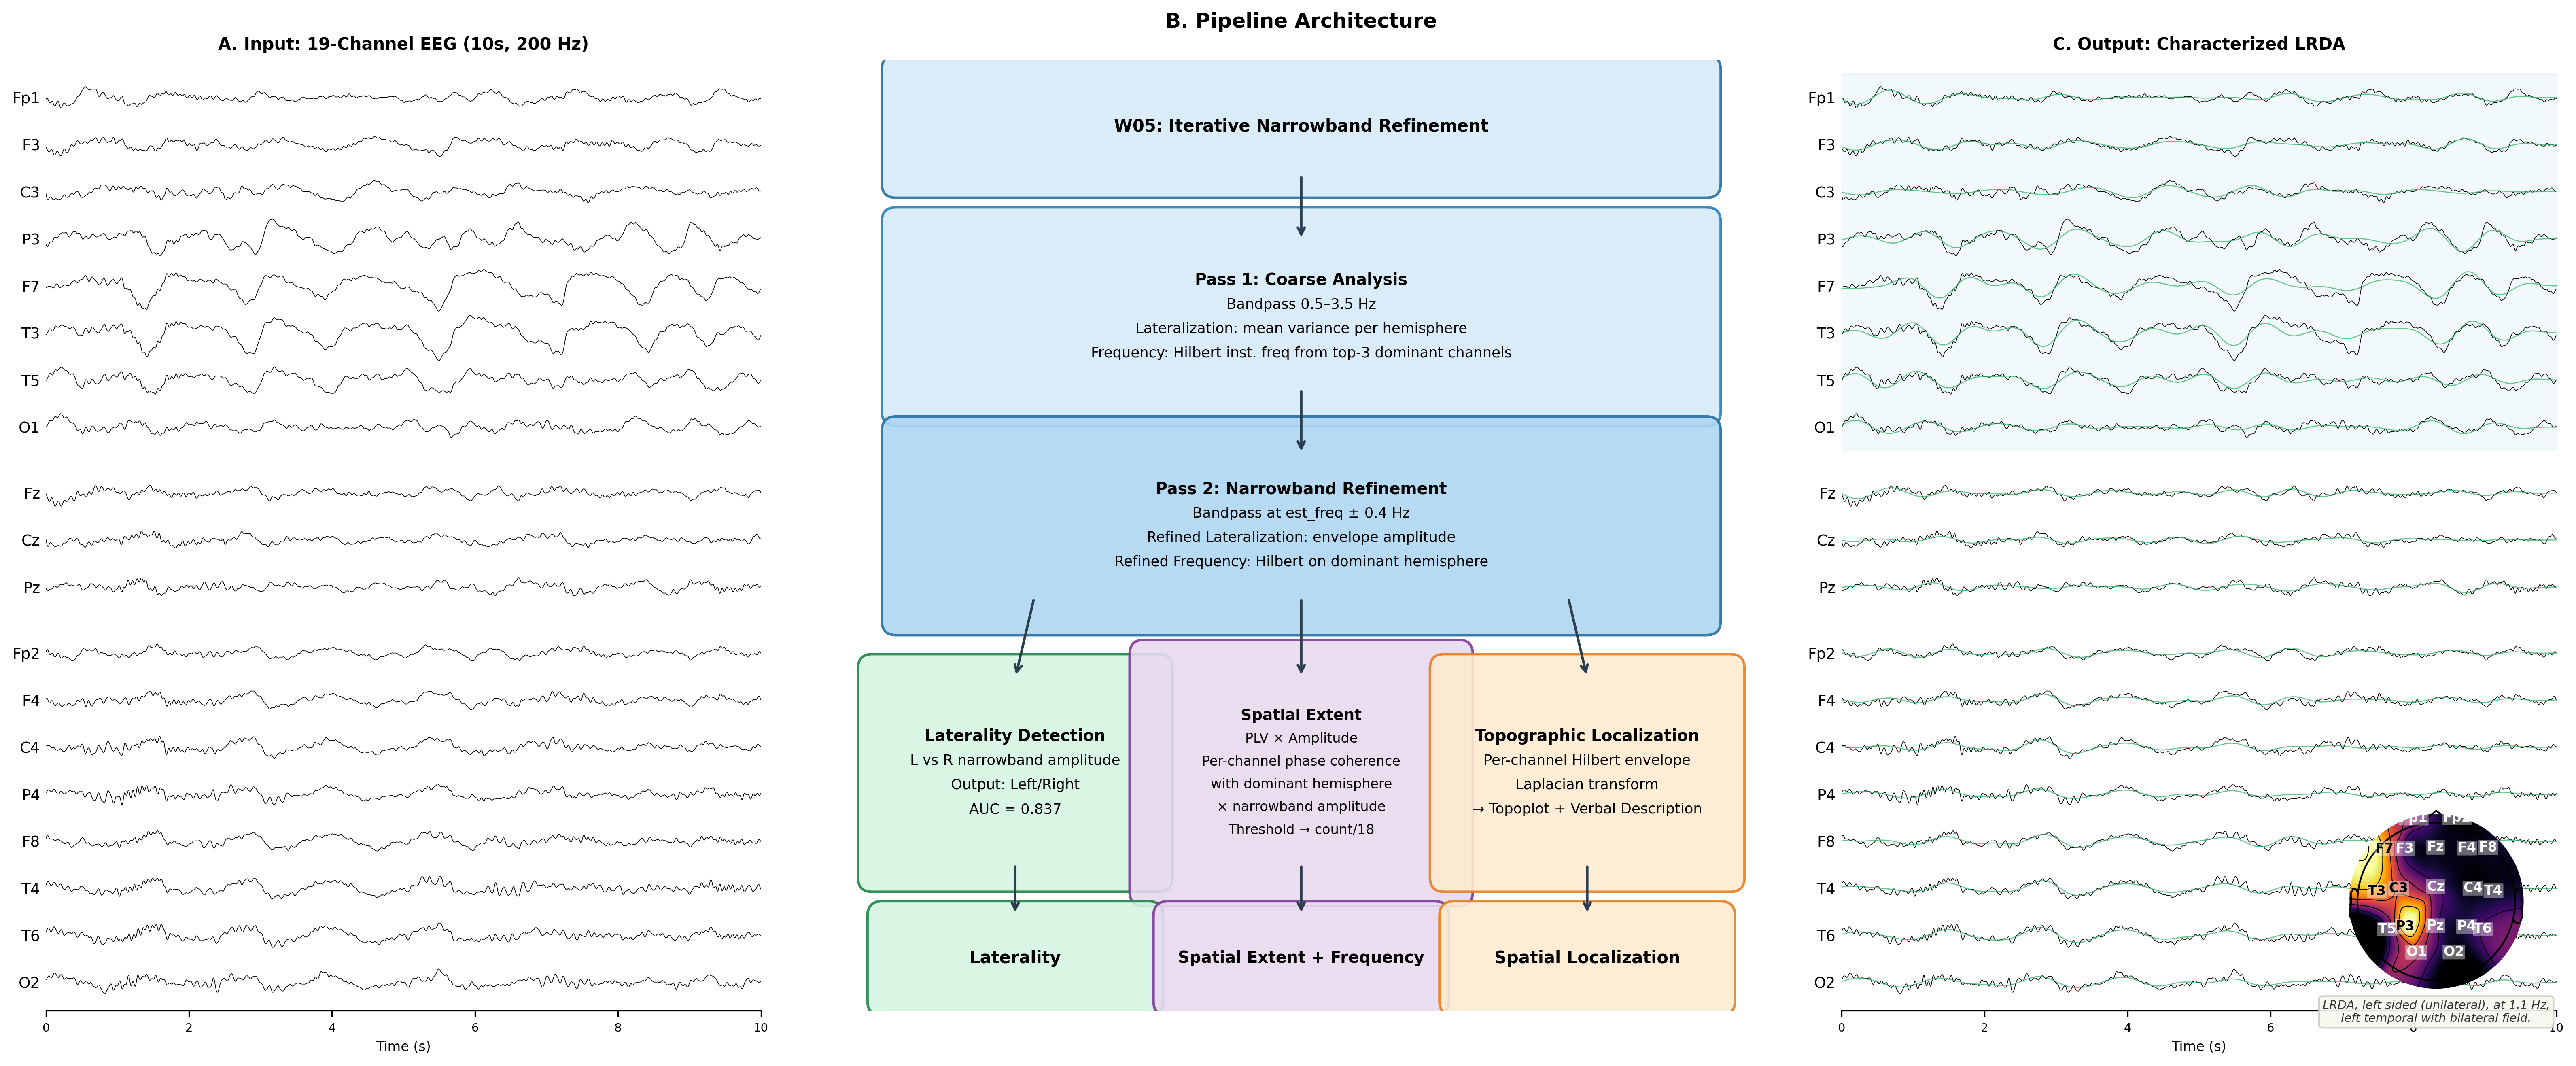
\includegraphics[width=\textwidth]{figures/fig3_rda_pipeline.png}
\caption{The RDA-Profiler uses two-pass iterative narrowband refinement to characterize continuous rhythmic activity. Three-panel overview of the rhythmic delta activity (RDA) characterization pipeline applied to an example LRDA segment, following the same layout as figure~\ref{fig:pd_pipeline}. \textbf{(A)}~Input: raw 19-channel average-reference EEG. \textbf{(B)}~Pipeline architecture: the NB-Hilbert iterative narrowband refinement algorithm performs two passes. Pass~1: coarse analysis with broadband (0.5--3.5~Hz) filtering, estimating lateralization via per-hemisphere mean variance and frequency via Hilbert instantaneous frequency from the top-3 dominant channels. Pass~2: narrowband filtering at the estimated frequency $\pm 0.4$~Hz, with envelope amplitude for refined lateralization and Hilbert frequency on the dominant hemisphere only. Three output branches produce laterality, spatial extent (via per-channel PLV with the dominant hemisphere), and frequency. \textbf{(C)}~Output: the same EEG with hemisphere shading, a Laplacian amplitude topoplot, and a verbal description. No discharge markers are shown, as RDA is a continuous rhythmic pattern. Scale bar: 100~$\mu$V.}
\label{fig:rda_pipeline}
\end{figure}

\subsubsection{NB-Hilbert: Iterative Narrowband Hilbert Refinement.}

Lateralization and frequency of RDA patterns were estimated using a two-pass iterative narrowband Hilbert refinement procedure (NB-Hilbert; identified as contest entry W05 in appendix~\ref{app:contest}). In the first pass, all 18 channels were bandpass-filtered at 0.5--3.5~Hz (third-order Butterworth, zero-phase). Coarse lateralization was determined by comparing mean broadband variance between left-hemisphere and right-hemisphere channel groups, and the dominant hemisphere was assigned to the side with higher variance. Coarse frequency was estimated using Hilbert-based instantaneous frequency analysis on the top-3 channels (by variance) of the dominant hemisphere, with the median of valid instantaneous frequency samples (within 0.3--4.0~Hz) taken as the estimate.

In the second pass, all channels were re-filtered using a narrow bandpass centered on the first-pass frequency estimate ($\pm 0.4$~Hz). Lateralization was refined by comparing the mean envelope amplitude (via Hilbert transform) between hemispheres, and frequency was re-estimated from the Hilbert instantaneous frequency of the top-3 narrowband channels on the refined dominant hemisphere. LRDA versus GRDA classification was based on an amplitude asymmetry index $A = |L_\mathrm{score} - R_\mathrm{score}| / (L_\mathrm{score} + R_\mathrm{score})$, with LRDA assigned when asymmetry exceeded a threshold calibrated against expert labels.

NB-Hilbert was selected as the best unified (lateralization plus frequency) method from a systematic contest of 76 algorithm variants evaluated on 4,253 RDA segments (1,295 LRDA, 2,958 GRDA; the subset of the 4,731 labeled non-excluded LRDA/GRDA segments in table~\ref{tab:dataset} for which valid 18-channel EEG data could be loaded from disk), achieving a lateralization AUC of 0.837 and frequency Spearman correlation of 0.635. Alternative methods evaluated included single-pass envelope amplitude (entry L24, AUC 0.826, no frequency output), PLV-selected channels (entry V04, AUC 0.809, frequency $\rho = 0.682$), and automatic channel selection with frequency consensus (entry V05, AUC 0.790, frequency $\rho = 0.686$). The iterative refinement approach provided the best lateralization performance by suppressing non-RDA activity through narrowband filtering tuned to the estimated pattern frequency. The full contest naming scheme is described in appendix~\ref{app:contest}.

\subsubsection{RDA-PLV: Spatial Extent.}

Spatial extent of RDA patterns was quantified using a PLV-amplitude product metric. Each bipolar channel was narrowband-filtered at the NB-Hilbert-estimated frequency ($\pm 0.4$~Hz). A reference signal was constructed as the mean of the top-3 narrowband channels on the dominant hemisphere. For each channel, the PLV with the reference was computed and multiplied by the normalized mean envelope amplitude. Channels with a PLV-amplitude product exceeding 0.15 were classified as involved, and spatial extent was reported as the fraction of involved channels. The PLV-amplitude product penalized channels with high PLV but negligible amplitude (noise-driven phase locking) and channels with high amplitude but poor phase coherence (non-rhythmic activity).

\subsection{BIPD Detection}
\label{sec:bipd}

Bilateral independent periodic discharges (BIPD)---defined by independent periodic discharge trains on each hemisphere with distinct timing sequences---were detected using a two-stage approach. In the first stage, the HemiCET-UNet + DP pipeline was run independently on each hemisphere, yielding two discharge time sequences. In the second stage, a gradient-boosted tree (GBT) classifier was trained on features computed from the bilateral timing sequences. Features included the frequency ratio between hemispheres, inter-pulse interval regularity (coefficient of variation), matched fraction (proportion of temporally coincident discharges within 100~ms), phase consistency (mean resultant length of the cross-hemisphere phase relationship), and asymmetry measures (sequence length ratio, frequency asymmetry, count asymmetry).

The GBT classifier was trained on synthetic data to overcome the rarity of confirmed BIPD cases (21 out of 198 candidates screened). Synthetic BIPD examples were constructed by pairing independent LPD sequences from different patients. Synthetic GPD examples were created by phase-shifting a single LPD sequence with random jitter ($\pm 25$~ms) to simulate synchronous bilateral discharges. The full 3-way classification (LPD vs.\ GPD vs.\ BIPD) used 29 features comprising 18 per-channel PD probabilities from ChannelPD-Net plus 11 timing-derived features.

\subsection{Statistical Analysis}
\label{sec:statistics}

Lateralization and classification performance was evaluated using the area under the receiver operating characteristic curve (AUC). Frequency estimation was assessed using Spearman rank correlation ($\rho$) and mean absolute error (MAE) against expert labels. Discharge timing accuracy was evaluated using F1 score (at $\pm 100$~ms tolerance), sensitivity, precision, and timing MAE (in milliseconds). Spatial localization was assessed using the Jaccard index (intersection over union) for PD region sets and the ICC(3,1) for spatial extent as a continuous measure. For inter-rater reliability analyses, 95\% confidence intervals were computed using bootstrap resampling (1,000 iterations).

Reported evaluation $n$ values are smaller than the corresponding label totals in table~\ref{tab:dataset} for two reasons: (i) under 5-fold patient-stratified cross-validation, an out-of-fold prediction is computed only for segments whose patient appears in a held-out fold (segments from patients used only for training appear in no fold's evaluation set), and (ii) frequency estimation is reported on the quality-filtered subset described above. The label-to-evaluation gap is therefore expected and method-specific; for example, the LPD versus GPD classifier is evaluated on the 7,037 (of 7,507 LPD+GPD) segments with both an out-of-fold prediction and the required RF feature set, the PD hemisphere lateralization task is evaluated on the 1,274 (of 1,336 LPD-laterality-annotated) segments with both an out-of-fold ChannelPD-Net prediction and a confirmed left/right label, and frequency-quality-filtered $n$ values are smaller than the expert-reviewed totals in table~\ref{tab:dataset} because the quality filter additionally requires a single-rater MW review or three-rater agreement.

%%%%%%%%%%%%%%%%%%%%%%%%%%%%%%%%%%%%%%%%%%%%%%%%%%
\section{Results}
\label{sec:results}

\subsection{Lateralization and Subtype Classification}
\label{sec:lateralization}

\textbf{PD lateralization.} ChannelPD-Net achieved a hemisphere lateralization AUC of 0.989 ($n = 1{,}274$) for determining whether PDs were left-dominant or right-dominant, based on the difference in mean PD probability between left and right hemisphere channels (table~\ref{tab:lateralization}). This near-ceiling performance indicated that the per-channel CNN reliably detected the lateralized nature of LPD patterns.

\textbf{LPD versus GPD classification.} A random forest (RF) classifier (300 trees) trained on 18 per-channel PD probabilities plus 8 handcrafted features achieved an AUC of 0.911 ($n = 7{,}037$) for distinguishing LPD from GPD. The features capturing spatial asymmetry in PD probability across channels were the primary drivers of classification performance.

\textbf{3-way PD classification (LPD vs.\ GPD vs.\ BIPD).} BIPD detection is a small, exploratory component of the present work: the dataset comprised 2{,}756 LPD, 2{,}298 GPD, and only 10 confirmed BIPD segments (21 confirmed BIPD cases were screened in total; 11 were retained for training and 10 used for held-out evaluation). The 3-way classifier incorporating timing-derived features reached a macro AUC of 0.862 ($n = 5{,}064$; per-class one-vs-rest AUCs LPD 0.832, GPD 0.835, BIPD 0.920); in the binary BIPD-vs-GPD comparison the classifier reached an AUC of 0.937 ($n = 2{,}308$). With only 10 held-out BIPD segments these AUC point estimates are highly uncertain: by the Hanley--McNeil approximation, 95\% confidence intervals are LPD $[0.821, 0.843]$, GPD $[0.824, 0.846]$, BIPD one-vs-rest $[0.804, 1.000]$, BIPD vs.\ GPD $[0.832, 1.000]$, and the overall macro AUC is dominated by the wide BIPD interval. The most discriminative features for BIPD detection were the matched fraction (proportion of cross-hemisphere coincident discharges within 100~ms) and the phase consistency between left and right hemisphere discharge trains, which capture the defining characteristic of temporal independence between hemispheres. We caution that all BIPD numbers reported here are preliminary; the synthetic-data training procedure (\S\ref{sec:bipd}) plausibly transfers to real BIPD because the timing-feature distinctions used by the classifier (independent vs.\ tightly time-locked discharge trains) are well-represented in the synthetic positive class, but a definitive evaluation will require a substantially larger held-out cohort of confirmed real BIPD segments.

\textbf{RDA lateralization (LRDA vs.\ GRDA).} The NB-Hilbert iterative narrowband refinement method achieved a lateralization AUC of 0.837 on 4,253 segments (1,295 LRDA, 2,958 GRDA) in the V5 lateralization contest (table~\ref{tab:lateralization}). This method outperformed 75 alternative approaches, including simple amplitude asymmetry (entry L24, AUC 0.826), PLV-based lateralization (entry V04, AUC 0.809), and various multi-channel Hilbert methods (AUC 0.790). The key to NB-Hilbert's superiority was that the narrowband filtering in pass~2 removed non-RDA activity, sharpening the lateralization signal. Clean per-segment labels proved critical: the same hemisphere-independent methods achieved only AUC 0.58 with noisy patient-level labels in earlier experiments, rising to 0.84 after label correction. Contest entry codes (L24, V04, etc.) refer to the V5 lateralization contest naming scheme described in appendix~\ref{app:contest}.

\begin{table}[t]
\caption{Lateralization and classification performance. AUC is reported with the Hanley--McNeil 95\% confidence interval. The 3-way and BIPD-vs-GPD rows include only $n=10$ confirmed BIPD segments and are reported as preliminary; their wide CIs reflect the small BIPD sample size, not the accuracy on the other classes.}
\centering
\begin{tabular}{l l l r}
\hline
Task & Method & AUC (95\% CI) & $N$ \\
\hline
PD hemisphere (L vs.\ R) & ChannelPD-Net mean probability & 0.989 [0.983, 0.995] & 1,274 \\
LPD vs.\ GPD & RF on channel probs + features & 0.911 [0.904, 0.918] & 7,037 \\
3-way macro (LPD/GPD/BIPD) & RF on channel probs + timing & 0.862$^\dagger$ & 5,064 \\
BIPD vs.\ GPD & Timing features (GBT) & 0.937 [0.83, 1.00]$^\dagger$ & 2,308 \\
LRDA vs.\ GRDA & NB-Hilbert (iterative narrowband) & 0.837 [0.823, 0.851] & 4,253 \\
\hline
\multicolumn{4}{l}{\footnotesize $^\dagger$Preliminary; only 10 confirmed BIPD segments in held-out evaluation (\S\ref{sec:limitations}).} \\
\end{tabular}
\label{tab:lateralization}
\end{table}

\subsection{Frequency Estimation}
\label{sec:frequency}

\textbf{PD frequency.} On quality-filtered segments, the PD-Profiler (IPI-derived frequency from HemiCET-UNet + DP) achieved Spearman correlations of 0.777 for LPD ($n = 1{,}155$, 95\% CI $[0.753, 0.799]$; MAE $= 0.165$~Hz, $[0.152, 0.179]$) and 0.829 for GPD ($n = 1{,}137$, $[0.810, 0.847]$; MAE $= 0.142$~Hz, $[0.083, 0.204]$) (table~\ref{tab:frequency}, figure~\ref{fig:freq_scatter}). These results represented substantial improvements over the signal-processing baseline of Tautan et al.~\cite{tautan2025}, which achieved correlations of 0.277 (LPD, MAE $= 0.505$~Hz) and 0.508 (GPD, MAE $= 0.339$~Hz) on the same labeled cohort -- approximately a 2.8-fold improvement on LPD and 1.6-fold on GPD. Patient-stratified paired bootstrap (1{,}000 resamples) of $\Delta\rho = \rho_\mathrm{alg} - \rho_\mathrm{Tautan}$ rejects $\Delta\rho = 0$ at $p<0.001$ on both subtypes (LPD $\Delta\rho = +0.501$, 95\% CI $[+0.435, +0.564]$; GPD $\Delta\rho = +0.321$, $[+0.197, +0.516]$); the corresponding MAE reductions (algorithm vs.\ Tautan) are $+0.340$~Hz and $+0.197$~Hz, both $p<0.001$.

The superior performance of IPI-derived frequency over direct CNN prediction ($\rho \approx 0.55$) or CNN+ACF ensemble ($\rho \approx 0.60$) confirmed that leveraging detected discharge timing for frequency estimation was substantially more accurate than spectral or regression-based approaches. The HemiCET-UNet + DP pipeline achieved a timing-derived frequency Spearman correlation of 0.891 on the 582 production evaluation cases, with a frequency MAE of 0.183~Hz.

\textbf{RDA frequency.} The NB-Hilbert iterative narrowband method (V12: pass-1 0.5--4.5~Hz, pass-2 narrowband half-width 0.5~Hz, top-3 channels, frequency cap 4.5~Hz) achieved Spearman correlations of 0.705 for LRDA ($n = 730$, 95\% CI $[0.666, 0.740]$; MAE $= 0.229$~Hz, $[0.203, 0.253]$) and 0.795 for GRDA ($n = 1{,}453$, $[0.775, 0.813]$; MAE $= 0.188$~Hz, $[0.164, 0.207]$) on quality-filtered segments (table~\ref{tab:frequency}, figure~\ref{fig:freq_scatter}). Tautan et al.\ achieved correlations of 0.077 (LRDA, MAE $= 0.624$~Hz) and 0.133 (GRDA, MAE $= 0.578$~Hz) on the same cohort -- a 9.2-fold improvement on LRDA and 6.0-fold on GRDA. The corresponding paired-bootstrap differences are LRDA $\Delta\rho = +0.620$, 95\% CI $[+0.515, +0.719]$, $p<0.001$; GRDA $\Delta\rho = +0.649$, $[+0.578, +0.712]$, $p<0.001$, with MAE reductions of $+0.390$~Hz and $+0.384$~Hz respectively (both $p<0.001$).

\begin{figure}[htbp]
\centering
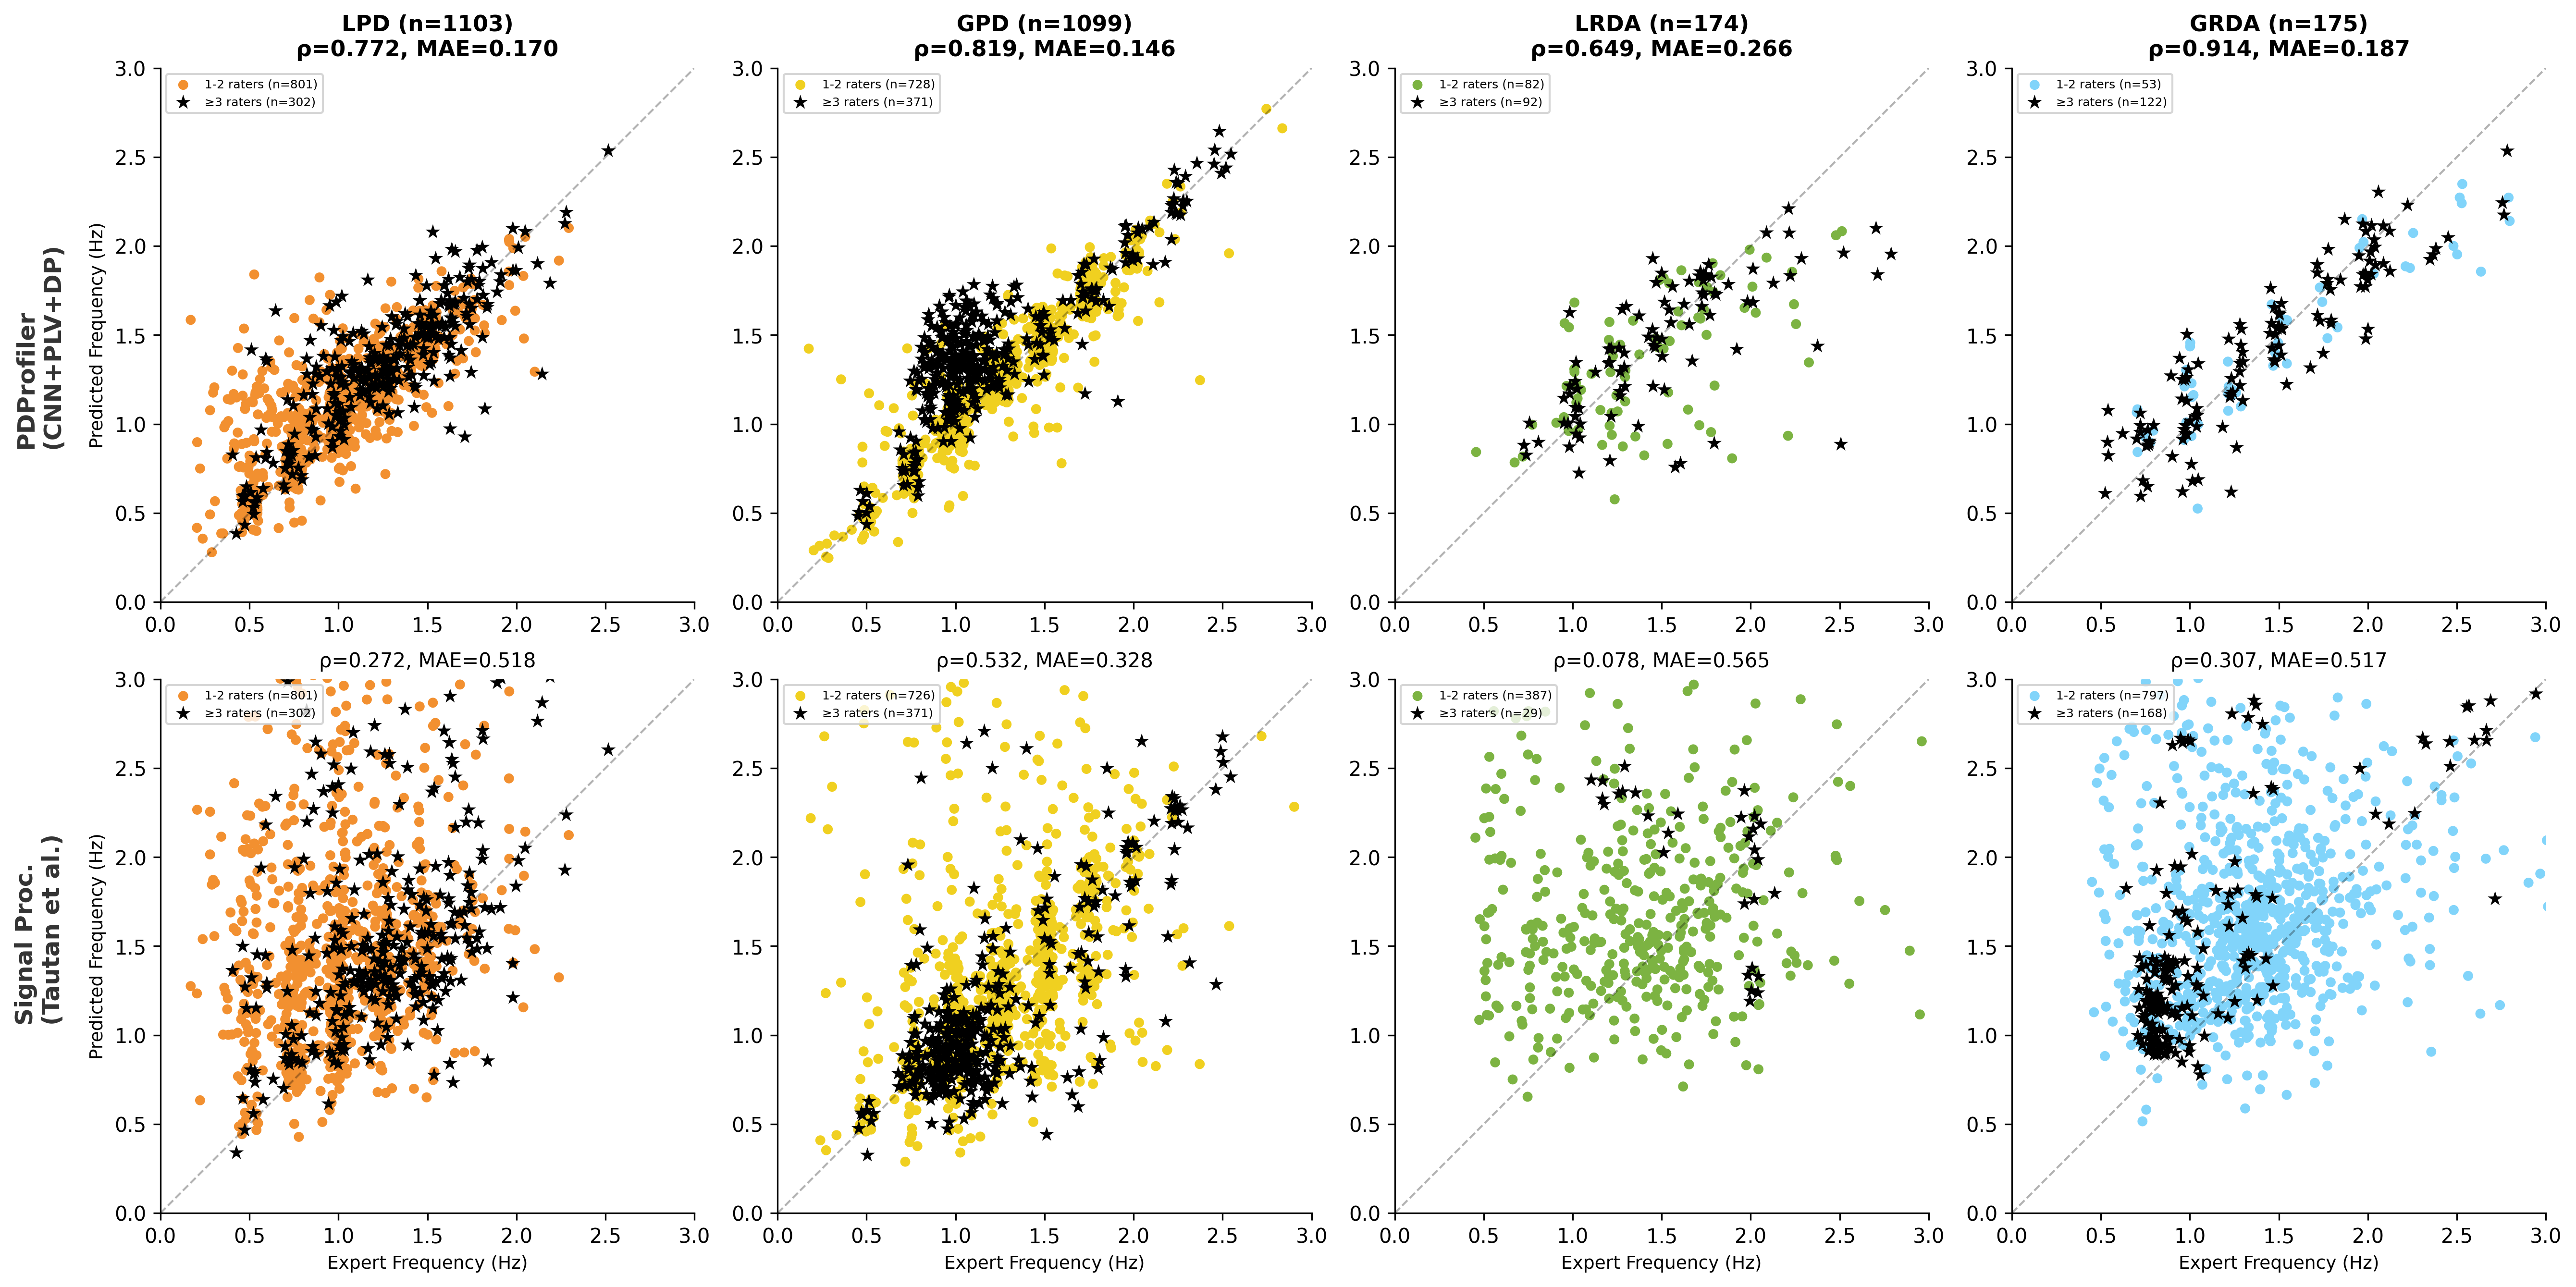
\includegraphics[width=\textwidth]{figures/fig4_frequency_scatter.png}
\caption{Algorithm frequency estimates correlate substantially more strongly with expert labels than the prior signal-processing state of the art. Scatter plots comparing algorithm-predicted frequency ($y$-axis) against expert-reviewed frequency ($x$-axis) for each subtype. Top row: present system (PD: CNN+ACF frequency prior refined by IPI from detected discharges; RDA: NB-Hilbert iterative narrowband Hilbert refinement, V12 hyperparameters). Bottom row: T\u{a}u\c{t}an et al.\ signal-processing baseline. Columns from left to right: LPD ($n = 1{,}155$; $\rho = 0.777$), GPD ($n = 1{,}137$; $\rho = 0.829$), LRDA ($n = 730$; $\rho = 0.705$), GRDA ($n = 1{,}453$; $\rho = 0.795$). Spearman correlation ($\rho$) and mean absolute error (MAE, in Hz) are shown for each panel; bootstrap 95\% CIs and paired Tautan-vs-algorithm $p$-values are reported in table~\ref{tab:frequency}. Expert frequency is the mean across available raters in labels.csv. The Tautan baseline was rerun on the same labeled cohort (per-row $n$ in the figure title differs slightly between methods because a small minority of segments produced an estimate from one method but not the other). Dashed diagonal line indicates perfect agreement.}
\label{fig:freq_scatter}
\end{figure}

\begin{figure}[htbp]
\centering
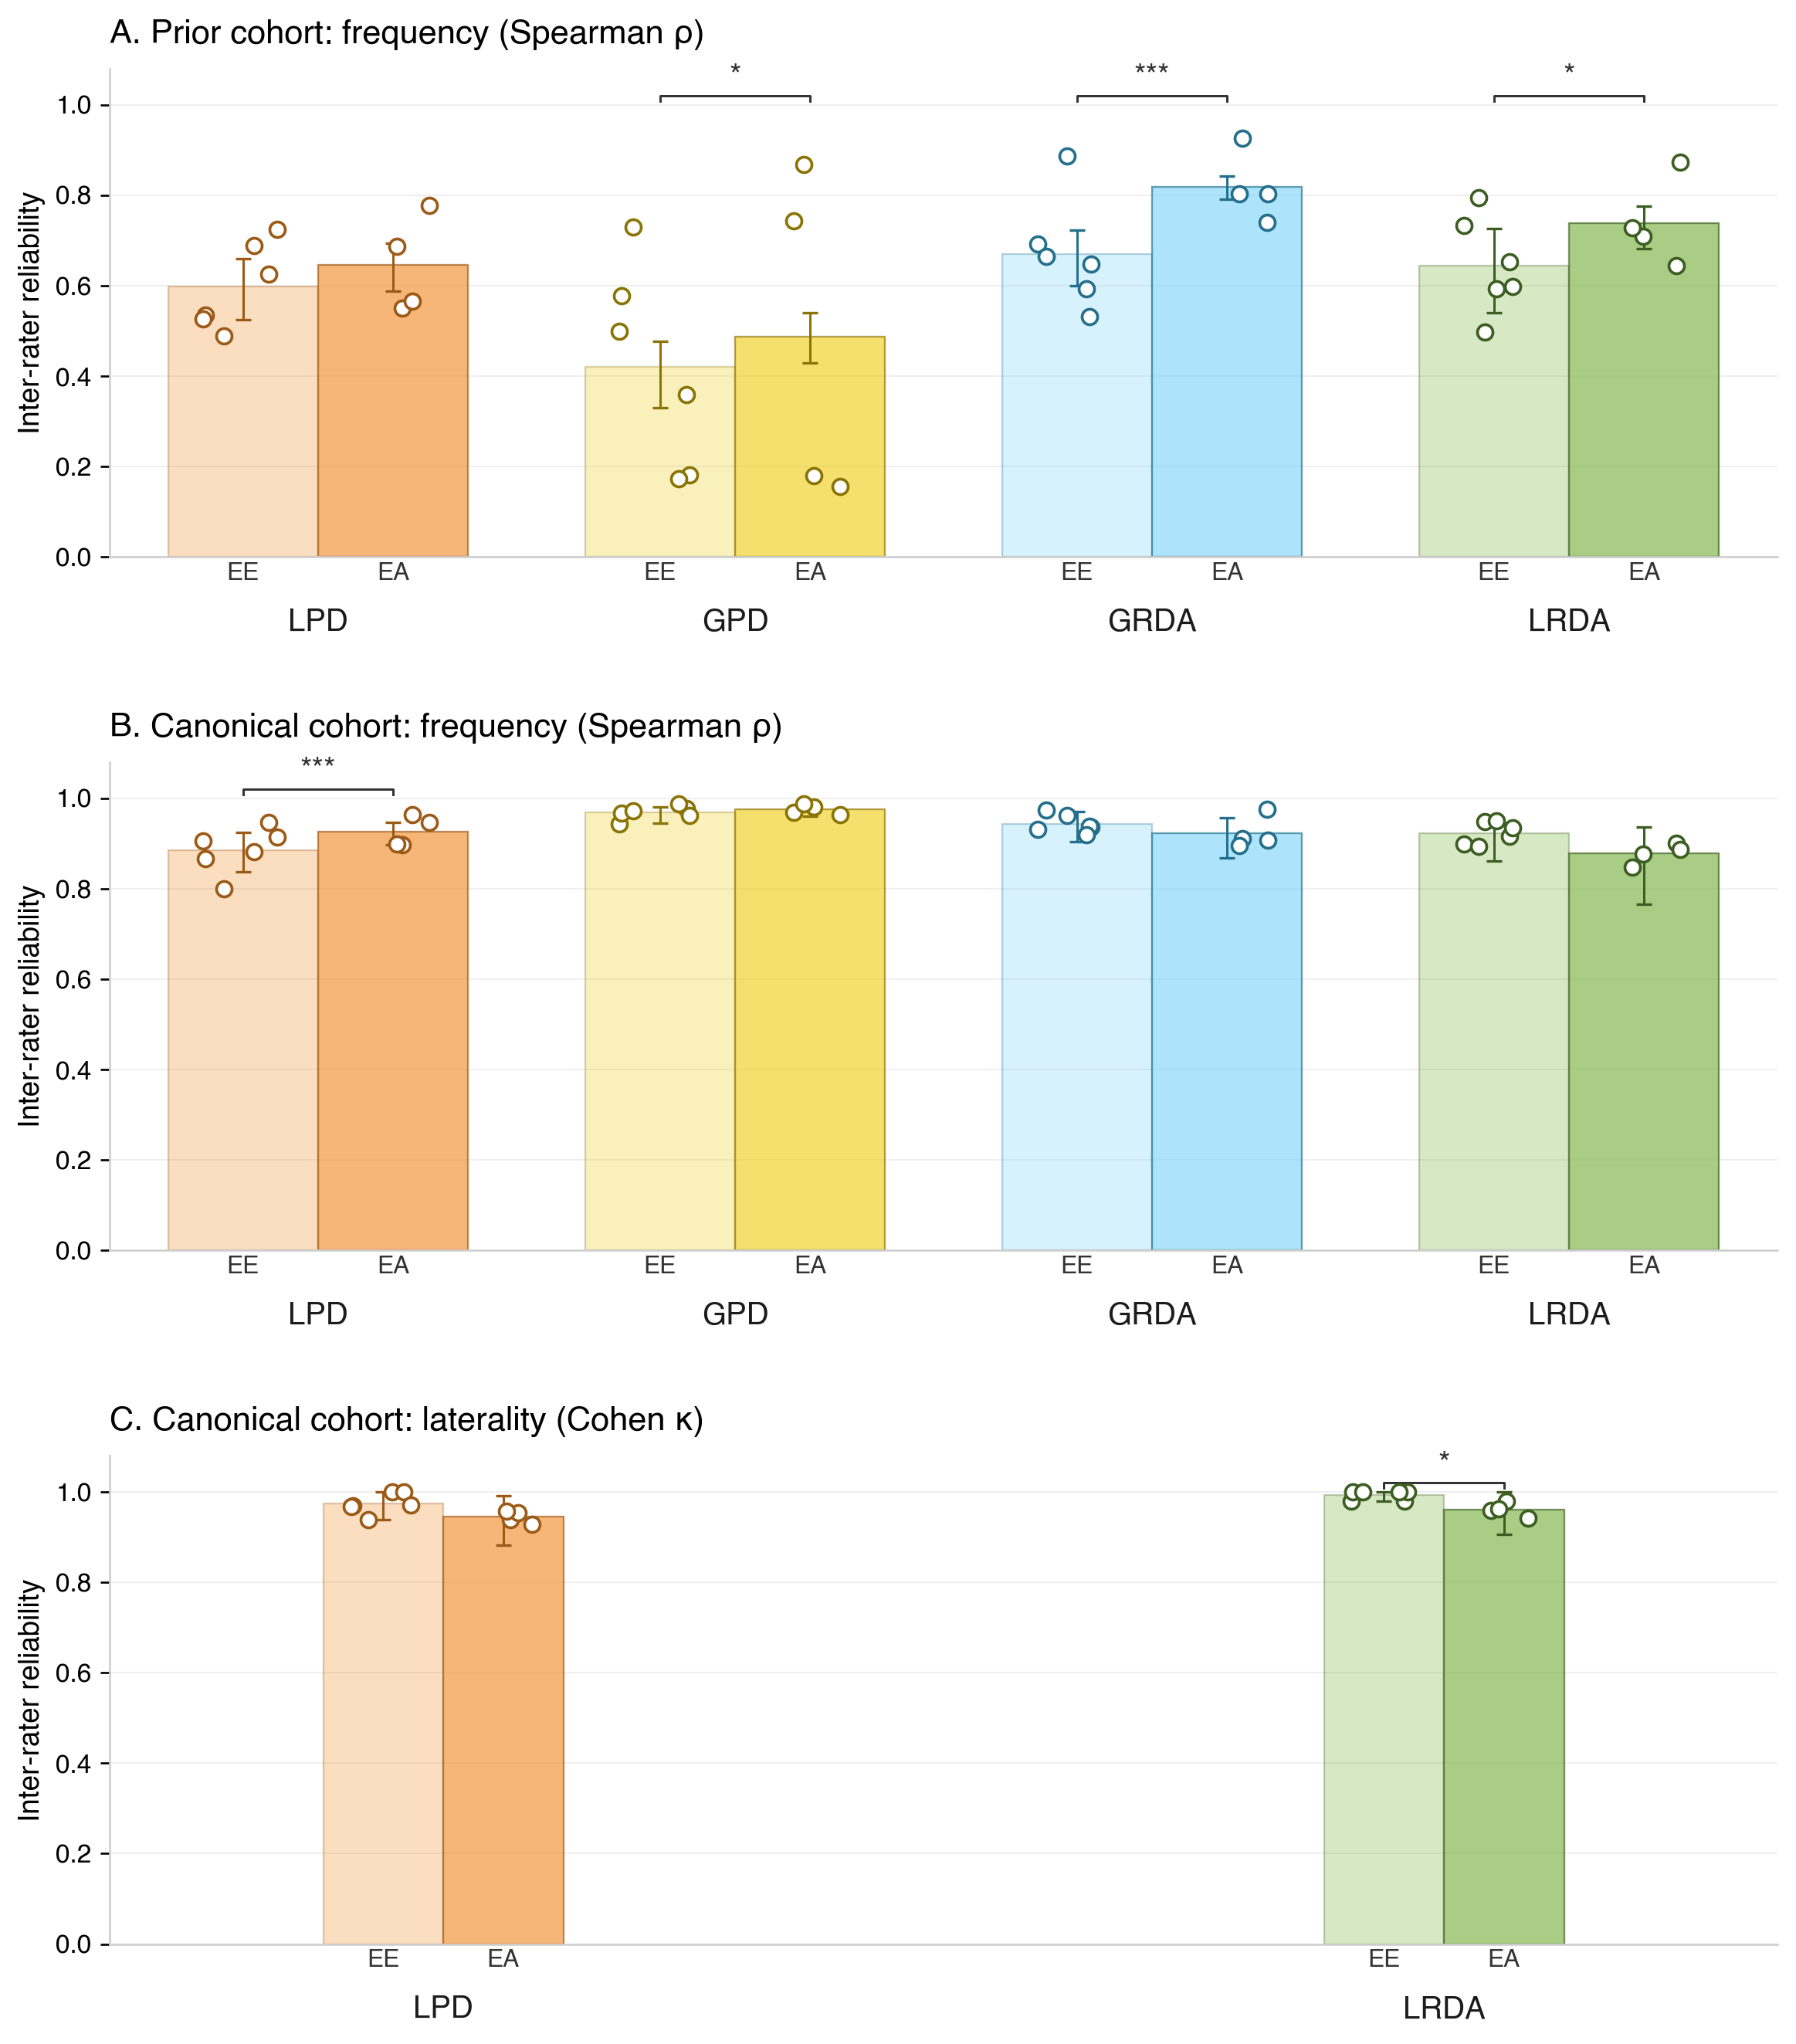
\includegraphics[width=\textwidth]{figures/fig5_irr_comparison.png}
\caption{Algorithm--expert agreement matches or exceeds the expert--expert ceiling on two independent 4-rater cohorts. Within each task the left bar shows mean expert--expert (EE) agreement across all $\binom{4}{2}=6$ within-cohort expert pairs, and the right bar shows mean expert--algorithm (EA) agreement across all 4 expert/algorithm pairs. Bar height is the mean across pairs computed by paired segment-level bootstrap (2{,}000 resamples); error bars are 95\% bootstrap CIs on that mean. Open circles overlaid on each bar are the per-pair point estimates (6 EE points, 4 EA points), with horizontal jitter for legibility. Bar color encodes IIIC pattern subtype using the same palette as figure~\ref{fig:freq_scatter} (LPD orange, GPD yellow, LRDA olive-green, GRDA sky-blue); the lighter shade is EE and the darker shade is EA. Significance brackets ($*$ $p<0.05$, $**$ $p<0.01$, $***$ $p<0.001$) are drawn only over comparisons where mean(EA)$-$mean(EE) reached significance under the paired bootstrap; non-significant comparisons (panel C, and several in panels A--B) are not annotated and are reported in the text. In every annotated comparison the algorithm direction was positive (EA $>$ EE). \textbf{(A) Prior 4-rater Tautan et al.~\cite{tautan2025} cohort (PH, LB, SZ, MW)}: frequency Spearman~$\rho$. PH, LB, and SZ produced their labels without the present interactive narrowband-overlay tools, so the EE ceiling on this cohort is correspondingly modest; laterality is not shown because PH and LB did not annotate laterality. \textbf{(B) Canonical 4-rater independent-expert cohort (MW, SZ, TZ, AS)} on 200 stratified segments per pattern subtype, restricted to segments where per-segment accepts exceeded rejects: frequency Spearman~$\rho$. \textbf{(C) Canonical cohort laterality (Cohen $\kappa$)} for LPD and LRDA only (GPD and GRDA are bilateral by definition). The algorithm uses V12 frequency estimation (NB-Hilbert with retuned hyperparameters: pass-1 0.5--4.5 Hz, pass-2 narrowband half-width 0.5 Hz, top-3 dominant-hemisphere channels averaged, frequency cap 4.5 Hz) and the V14 amplitude/rhythmicity hybrid laterality rule (default to the V12 amplitude call; override only when four amplitude-normalized rhythmicity measures -- per-channel Q-factor, within-hemisphere phase-locking value, narrowband peak-amplitude consistency, and spectral peak prominence -- \emph{unanimously} disagree with the amplitude call). Per-pair ICCs and MAEs are reported in the main text and in table~\ref{tab:phlbsz_cohort}.}
\label{fig:irr_main}
\end{figure}

\textbf{Validation against the prior 4-rater cohort (Tautan et al.\ 2025 + MW).}
As a check on a different annotation cohort, we evaluated the algorithm against the four expert raters (PH, LB, SZ, MW) on the Tautan et al.~\cite{tautan2025} dataset, where PH/LB/SZ produced their labels without the present interactive narrowband-overlay tools (the labels are therefore noisier than the canonical cohort by construction). Mean agreement across the six within-role expert--expert pairs and the four expert--algorithm pairs (table~\ref{tab:phlbsz_cohort}) shows that the algorithm meets or exceeds expert--expert reliability on three of the four subtypes: mean expert--algorithm ICC~0.69 vs.\ mean expert--expert ICC~0.64 on LRDA, mean EA~0.86 vs.\ mean EE~0.84 on GRDA, and mean EA~0.57 vs.\ mean EE~0.50 on LPD. On GPD the algorithm is approximately at the expert--expert level (mean EA~0.43 vs.\ mean EE~0.47); per-pair detail shows that the algorithm tracks SZ and MW tightly (ICC~0.83 and 0.85 respectively) but disagrees more substantially with PH and LB (ICCs~0.06 and $-0.07$), suggesting a scoring-convention difference on this subtype that warrants future investigation. The Tautan et al.\ signal-processing baseline is uniformly weaker than the present algorithm on this cohort (mean expert--Tautan ICC: LPD~0.10, GPD~0.36, LRDA~$-0.21$, GRDA~0.17).

\begin{table}[t]
\caption{Algorithm validation on the prior 4-rater cohort (raters PH, LB, SZ, MW) labeled on the Tautan et al.~\cite{tautan2025} dataset. Mean across the within-role pairs ($\binom{4}{2}=6$ expert--expert pairs, 4 expert--algorithm pairs, 4 expert--Tautan pairs). The PH/LB/SZ labels were produced without the interactive narrowband-overlay tools introduced here and are noisier than the canonical cohort by construction.}
\label{tab:phlbsz_cohort}
\centering
\small
\begin{tabular}{l | c c c | c c c | c c c}
\hline
& \multicolumn{3}{c|}{Expert--Expert} & \multicolumn{3}{c|}{Expert--Algorithm} & \multicolumn{3}{c}{Expert--Tautan} \\
Task & ICC & $\rho$ & MAE & ICC & $\rho$ & MAE & ICC & $\rho$ & MAE \\
\hline
LPD freq  & 0.50 & 0.62 & 0.29 & \textbf{0.57} & \textbf{0.63} & \textbf{0.25} &  0.10 & 0.23 & 0.50 \\
GPD freq  & 0.47 & 0.41 & 0.26 & 0.43 & 0.48 & 0.31 &  0.36 & 0.38 & 0.31 \\
LRDA freq & 0.64 & 0.71 & 0.22 & \textbf{0.69} & \textbf{0.73} & \textbf{0.20} & $-0.21$ & 0.15 & 0.74 \\
GRDA freq & 0.84 & 0.76 & 0.16 & \textbf{0.86} & \textbf{0.84} & 0.17 &  0.17 & $-0.03$ & 0.57 \\
\hline
\end{tabular}
\end{table}

\textbf{Re-evaluation against independent raters.}
\label{sec:reeval}
The independent-expert task described above included 200 segments per subtype (LPD, GPD, LRDA, GRDA), each scored independently by MW, SZ, TZ, and AS. Under the canonical majority-accept consensus rule (per-segment accepts $>$ per-segment rejects across the four raters), per-task eligible segment counts are LPD~177, GPD~191, LRDA~104, GRDA~134; per-pair sample sizes within each task are reported in figure~\ref{fig:irr_main}.

For LPD frequency, the four expert--algorithm ICCs are 0.875 (MW), 0.976 (SZ), 0.923 (TZ), and 0.950 (AS) for a mean of 0.931, against a mean expert--expert ICC of 0.897 across the six EE pairs; the difference is significantly favorable to the algorithm ($\Delta=+0.034$, 95\% CI $[+0.016,+0.055]$, $p<0.001$). For GPD frequency, expert--algorithm ICCs are 0.963 (MW), 0.987 (SZ), 0.977 (TZ), and 0.994 (AS) for a mean of 0.980, marginally above the mean EE ICC of 0.973 ($\Delta=+0.007$, $p=0.061$, n.s.). For GRDA frequency, expert--algorithm ICCs are 0.903 (MW), 0.989 (SZ), 0.899 (TZ), and 0.913 (AS) for a mean of 0.926 against EE 0.946 ($\Delta=-0.020$, $p=0.056$, n.s.).

For LRDA, the originally chosen NB-Hilbert hyperparameters (pass-1 bandpass 0.5--3.5~Hz; pass-2 narrowband half-width 0.4~Hz) had been selected during the early algorithm contest using a small three-rater cohort. With the expanded majority-accept consensus dataset now available, we re-tuned these hyperparameters via a 192-point grid search (pass-1 bandpass upper $\in\{3.5,4.0,4.5,5.0\}$~Hz; pass-2 half-width $\in\{0.3,0.4,0.5,0.6\}$~Hz; top-$K$ channels $\in\{2,3,4,5\}$; frequency search cap $\in\{3.5,4.0,4.5\}$~Hz). The retuned configuration (pass-1 0.5--4.5~Hz; pass-2 half-width 0.5~Hz; top-3 channels; cap 4.5~Hz) reached LRDA expert--algorithm ICCs of 0.829 (MW), 0.882 (SZ), 0.852 (TZ), and 0.831 (AS) for a mean of 0.854 against expert--expert mean 0.914 ($\Delta=-0.055$, 95\% CI $[-0.179,+0.017]$, $p=0.209$, n.s.). For LRDA laterality, the original W05 rule lateralizes by amplitude (which hemisphere has more narrowband envelope amplitude at the estimated rhythm frequency); this is fallible by construction whenever artifact, slow drift, or asymmetric volume conduction inflates one hemisphere's amplitude even when the rhythm itself is on the other side. We therefore developed V14, a hybrid that defaults to the amplitude rule but overrides it whenever four amplitude-normalized rhythmicity measures (per-channel Q-factor, within-hemisphere phase-locking value, narrowband peak-amplitude consistency, and spectral peak prominence) \emph{unanimously} disagree with the amplitude call. The resulting LRDA-laterality expert--algorithm $\kappa$'s are 0.942 (MW), 0.979 (SZ), 0.960 (TZ), and 0.962 (AS) for a mean of 0.961 against expert--expert mean 0.986 ($\Delta=-0.026$, $p=0.383$, n.s.).

To formally test whether the algorithm--expert agreement differs from expert--expert agreement on each task, we performed a paired segment-level bootstrap (2000 resamples) of $\Delta = \mathrm{mean}_\mathrm{EA} - \mathrm{mean}_\mathrm{EE}$ (sign-corrected so positive favors the algorithm). The algorithm exceeded the expert--expert ceiling at significance only on LPD frequency (ICC $\Delta=+0.034$, $p<0.001$; Spearman $\Delta=+0.041$, $p<0.001$); was statistically indistinguishable from the expert ceiling on GPD frequency ($p=0.061$), GRDA frequency ($p=0.056$), LRDA frequency ($p=0.209$), LPD laterality ($p=0.467$), and LRDA laterality ($p=0.383$); and was significantly below the expert ceiling only on RDA MAE (LRDA $p=0.001$, GRDA $p<0.001$). The MAE gap reflects a small constant offset between algorithm and expert frequency estimates that is invisible to ICC and Spearman; the algorithm tracks the rank ordering of expert frequencies tightly but with a $\sim$0.05--0.06~Hz residual bias on RDA tasks. A summary visualization with paired EE/EA bars, 95\% CIs on the means, and significance markers is shown in figure~\ref{fig:irr_main}.

\begin{figure}[htbp]
\centering
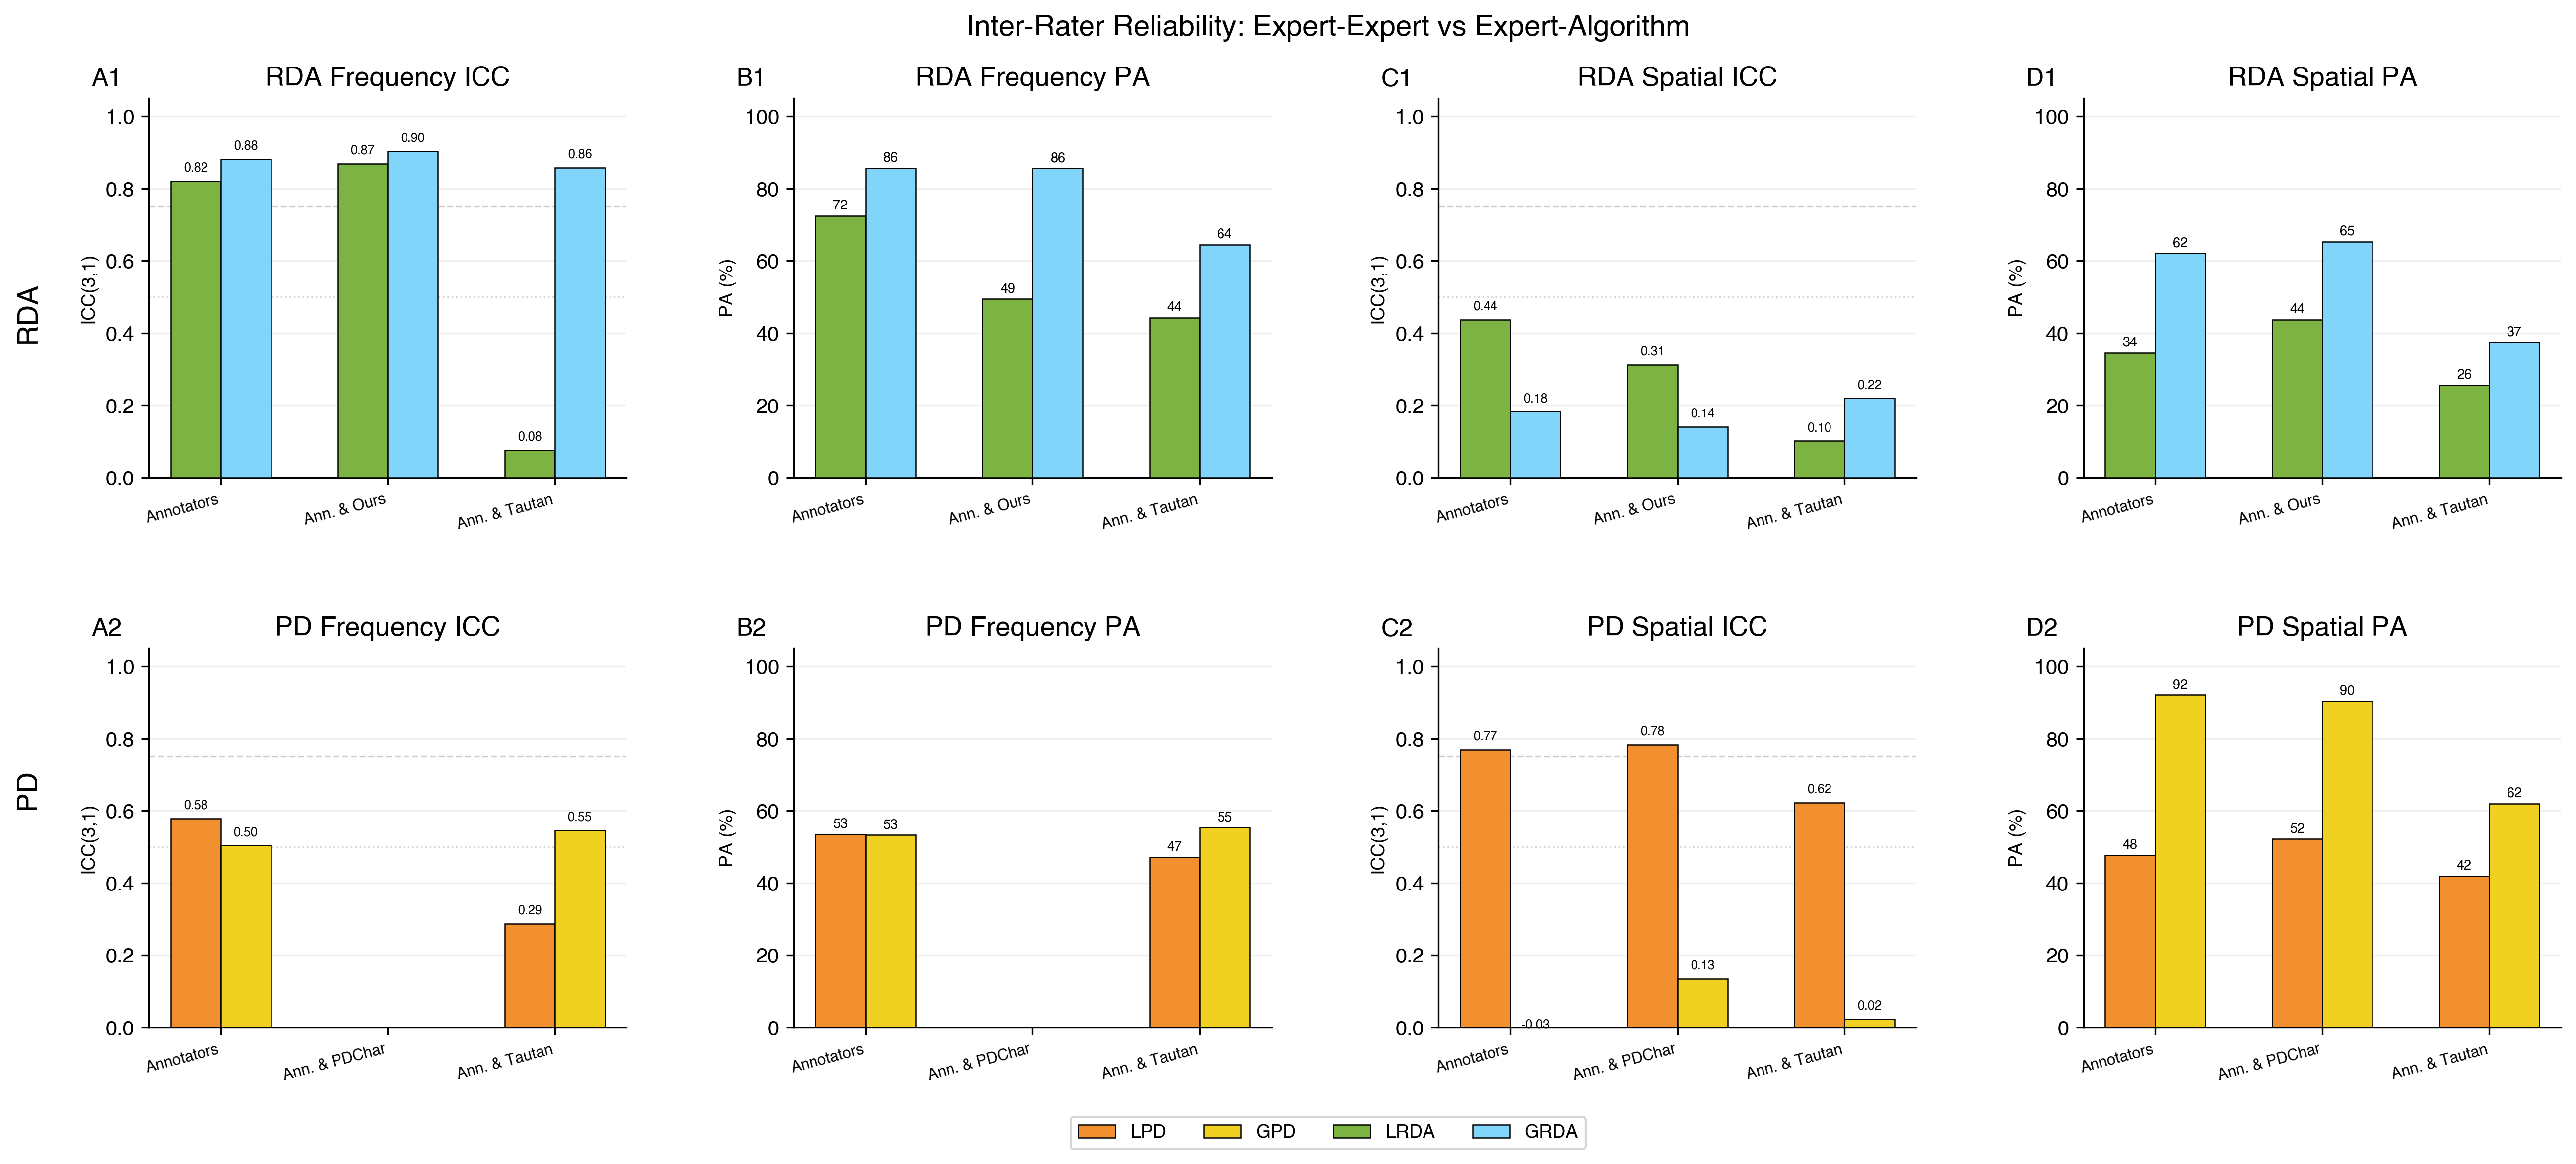
\includegraphics[width=\textwidth]{figures/figS1_irr_comparison.png}
\caption{Inter-rater reliability comparison: expert--expert versus algorithm--expert. Bar charts comparing ICC(3,1) and percentage agreement for frequency and spatial extent estimation. Top row: RDA (LRDA + GRDA combined). Bottom row: PD (LPD + GPD combined). Three conditions compared: expert--expert agreement (blue), present system (orange), and T\u{a}u\c{t}an et al.\ (green). NB-Hilbert (RDA-Profiler) for RDA frequency achieves ICC $= 0.860$, slightly exceeding expert--expert ICC $= 0.852$. PD-Profiler for PD spatial extent achieves ICC $= 0.852$ after threshold optimization, exceeding expert--expert ICC $= 0.845$. T\u{a}u\c{t}an et al.~\cite{tautan2025} included for direct comparison.}
\label{fig:irr}
\end{figure}

\begin{table}[t]
\caption{Frequency estimation performance on the labels.csv-canonical quality-filtered cohort. Algorithm $\rho$ 95\% CIs are computed via the Fisher $z$-transform and algorithm MAE 95\% CIs via patient-stratified bootstrap (1{,}000 resamples). The right-most column reports the two-sided patient-stratified paired-bootstrap test of $\Delta\rho = \rho_\mathrm{alg}-\rho_\mathrm{Tautan}$ on segments where both methods produced an estimate; $p<0.001$ on every subtype, with bootstrap 95\% CIs on $\Delta\rho$ never crossing zero (\S\ref{sec:frequency}).}
\centering
\small
\begin{tabular}{l r l l c c c}
\hline
Subtype & $N$ & Algorithm $\rho$ [95\% CI] & Algorithm MAE [95\% CI] & Tautan $\rho$ & Tautan MAE & $p_{\Delta\rho}$ \\
\hline
LPD  & 1{,}155 & 0.777 [0.753, 0.799] & 0.165 [0.152, 0.179] & 0.277 & 0.505 & $<\!0.001$ \\
GPD  & 1{,}137 & 0.829 [0.810, 0.847] & 0.142 [0.083, 0.204] & 0.508 & 0.339 & $<\!0.001$ \\
LRDA & 730     & 0.705 [0.666, 0.740] & 0.229 [0.203, 0.253] & 0.077 & 0.624 & $<\!0.001$ \\
GRDA & 1{,}453 & 0.795 [0.775, 0.813] & 0.188 [0.164, 0.207] & 0.133 & 0.578 & $<\!0.001$ \\
\hline
\end{tabular}
\label{tab:frequency}
\end{table}

\textbf{Label quality analysis.} The quality of ground-truth frequency labels substantially influenced apparent algorithm performance. Segments with less than 60\% expert agreement on pattern classification exhibited 2.4-fold higher frequency discrepancy between algorithm and expert than segments with 100\% agreement. When MW re-reviewed all cases where the algorithm--expert frequency discrepancy exceeded 0.5~Hz, the original MW label was corrected in favor of the algorithm estimate in 94\% of PD cases and 61\% of RDA cases. This bidirectional quality improvement---algorithm predictions revealing annotation errors, which in turn improved the evaluation benchmark---was a recurring theme throughout development.

\subsection{Discharge Timing}
\label{sec:timing}

On 582 evaluation cases at $\pm 100$~ms tolerance, the HemiCET-UNet + DP pipeline achieved a discharge detection F1 of 0.889 (sensitivity 0.921, precision 0.859; table~\ref{tab:timing}). The 582 evaluation cases were a quality-filtered subset of the 675 training segments described in section~\ref{sec:pd_pipeline}, excluding cases without a documented discharge-timing review pass. The median timing MAE was 1.0~ms, indicating that detected discharges were localized to within a single sample (5~ms at 200~Hz) of the expert-annotated timing. The IPI-derived frequency from detected discharges achieved Spearman $\rho$ of 0.891 with expert-reviewed frequency.

This performance substantially exceeded two earlier pipeline versions: the full 18-channel pipeline (F1 $= 0.726$, timing MAE $= 17.7$~ms) and the per-hemisphere baseline using handcrafted evidence only (F1 $= 0.719$, timing MAE $= 19.4$~ms). The HemiCET approach also exceeded an Oracle baseline that used expert-annotated frequency as the DP prior with handcrafted evidence (F1 $= 0.664$, timing MAE $= 10.9$~ms). This finding demonstrated that learned evidence from the 8-channel HemiCET-UNet was superior to handcrafted features, more than compensating for imperfect frequency knowledge. The 8-channel hemisphere design outperformed the full 18-channel approach because it avoided noise from the uninvolved hemisphere (for LPD) and learned cross-channel patterns within a hemisphere directly.

\begin{table}[t]
\caption{Discharge timing performance.}
\centering
\begin{tabular}{l c c c c c}
\hline
Method & F1 & Sensitivity & Precision & Freq $\rho$ & Timing MAE (ms) \\
\hline
HemiCET-UNet + DP (production) & 0.889 & 0.921 & 0.859 & 0.891 & 1.0 \\
Oracle (expert freq + HPP) & 0.664 & 0.569 & 0.799 & 0.910 & 10.9 \\
Full 18-channel pipeline & 0.726 & 0.722 & 0.730 & 0.765 & 17.7 \\
Per-hemisphere baseline & 0.719 & 0.724 & 0.715 & 0.778 & 19.4 \\
\hline
\end{tabular}
\label{tab:timing}
\end{table}

\subsection{Spatial Localization}
\label{sec:spatial}

\subsubsection{PD Spatial Localization.}

\textbf{Discharge-locked topographic localization.} The primary spatial localization method for PDs computed the mean discharge topography using the two-pass Laplacian--GFP alignment procedure described in section~\ref{sec:pd_pipeline}. Representative topographic maps are shown in figures~\ref{fig:lpd_char}--\ref{fig:gpd_char}. The Laplacian transform sharpened spatial resolution by removing volume-conducted contributions, producing focal peaks corresponding to cortical generators. The GFP-squared weighting reduced the effective contribution of phantom discharges by a factor of 4--10 relative to uniform averaging, and the two-pass alignment reduced cross-epoch jitter by approximately 8--12~ms compared to single-pass GFP alignment.

\textbf{Spatial extent (Jaccard agreement).} The Hybrid-PLV spatial method was evaluated against three expert raters (LB, PH, SZ) on PD segments with 3-rater ground truth (table~\ref{tab:spatial_jaccard}; per-subtype scatter in supplementary figure~\ref{fig:spatial_scatter}). The choice of binarization threshold influenced model--expert agreement (supplementary figure~\ref{fig:threshold_sweep}); at the optimized threshold of 0.38, the mean model--expert Jaccard index was 0.731 ($\pm 0.076$), compared to a mean expert--expert Jaccard of 0.751 ($\pm 0.025$), representing 97.3\% of human inter-rater agreement. Notably, the model-PH agreement (Jaccard 0.837) exceeded all expert--expert pairs (maximum: LB--SZ at 0.773), indicating that the model acted as a ``virtual fourth rater'' with agreement patterns within the range of expert variation.

\begin{table}[t]
\caption{PD spatial inter-rater agreement (Jaccard, threshold $= 0.38$).}
\centering
\begin{tabular}{l r r r r}
\hline
 & LB & PH & SZ & Model \\
\hline
LB & 1.000 & 0.762 & 0.773 & 0.693 \\
PH & 0.762 & 1.000 & 0.716 & 0.837 \\
SZ & 0.773 & 0.716 & 1.000 & 0.662 \\
Model & 0.693 & 0.837 & 0.662 & 1.000 \\
\hline
\end{tabular}
\label{tab:spatial_jaccard}
\end{table}

After threshold optimization (threshold $= 0.62$) and quality filtering (excluding SZ spatial\_extent $= 0$ entries), the PD-Profiler spatial ICC was 0.852, exceeding the expert-expert ICC of 0.845 (figure~\ref{fig:irr}). In comparison, Tautan et al.~\cite{tautan2025} achieved a PD spatial ICC of 0.764 on the same segments.

\subsubsection{RDA Spatial Extent.}

The RDA-PLV method achieved an ICC of 0.371 when the algorithm was treated as a fourth rater alongside the three experts, compared to an expert-expert ICC of 0.373 ($n = 211$ segments with 3-rater spatial ground truth). The algorithm MAE of 0.215 was better than some expert-expert pairs (e.g., LB vs.\ SZ MAE $= 0.484$). Tautan et al.\ achieved an RDA spatial ICC of 0.215, substantially below both expert agreement and the present method.

The low absolute ICC values (approximately 0.37) for RDA spatial extent---for both the algorithm and expert raters---reflected the inherent difficulty of the verbal region-counting task. Unlike PD spatial localization, where discrete discharges create identifiable transients, RDA produces continuous rhythmic activity whose boundaries are gradual and subjective. The near-parity between algorithm and expert ICC indicated that the PLV-amplitude method captured the same information experts used when judging spatial extent. We treat the low absolute reliability as evidence that the categorical labeling task is itself noisy rather than as a target to be chased further; the principled spatial output of the system is the discharge-locked topographic map, as discussed in \S\ref{sec:label_quality}.

\subsection{End-to-End Characterization Examples}
\label{sec:examples}

Figures~\ref{fig:lpd_char}--\ref{fig:grda_char} present representative characterization examples for all four subtypes at three difficulty levels (easy, medium, hard), selected to span the range of inter-rater agreement. Each example shows the 19-channel EEG with pipeline outputs overlaid: detected discharge times (red dashed lines, PD only), hemisphere shading (light blue), Laplacian topographic map (inferno colormap), and ACNS 2021 verbal description.

For LPD examples (figure~\ref{fig:lpd_char}), the easy case (IIIC agreement $\geq 95\%$) exhibited clear, stereotyped discharges with unambiguous lateralization and a sharp focal maximum in the topographic map. The medium case (70--80\% agreement) showed recognizable periodicity with some morphological variability; the pipeline correctly lateralized and detected most discharges, though one or two marginal peaks were missed. The hard case (45--60\% agreement) featured subtle, atypical discharges where expert raters themselves disagreed; the pipeline produced a reasonable characterization, though the topographic map was more diffuse, reflecting the ambiguity of the pattern.

For GPD examples (figure~\ref{fig:gpd_char}), discharge markers spanned both hemispheres, and the topographic maps showed bilateral, often frontally predominant distributions. For LRDA and GRDA examples (figures~\ref{fig:lrda_char}--\ref{fig:grda_char}), no discharge markers were shown (RDA being a continuous rhythmic pattern), but hemisphere shading and amplitude topographic maps correctly identified the spatial distribution.

\begin{figure}[htbp]
\centering
\includegraphics[width=\textwidth]{figures/fig6_lpd_characterization.png}
\caption{LPD characterization examples at three difficulty levels. Three representative lateralized periodic discharge (LPD) cases selected to span the range of inter-rater agreement. Each row shows one case with: (left) 19-channel average-reference EEG (10 seconds, bandpass 0.3--50~Hz, amplitude clipped at $\pm 250$~$\mu$V) with detected discharge times marked as red dashed vertical lines on the involved hemisphere and light blue shading indicating the lateralized side; (right) Laplacian topoplot (inferno colormap) with electrode labels, and ACNS 2021 verbal description. Top: easy case (agreement $\geq 95\%$). Middle: medium case (agreement 70--80\%). Bottom: hard case (agreement 45--60\%). Scale bar: 100~$\mu$V.}
\label{fig:lpd_char}
\end{figure}

\begin{figure}[htbp]
\centering
\includegraphics[width=\textwidth]{figures/fig7_gpd_characterization.png}
\caption{GPD characterization examples at three difficulty levels. Three representative generalized periodic discharge (GPD) cases, following the same format as figure~\ref{fig:lpd_char}. Discharge markers span both hemispheres, reflecting the generalized distribution. Scale bar: 100~$\mu$V.}
\label{fig:gpd_char}
\end{figure}

\begin{figure}[htbp]
\centering
\includegraphics[width=\textwidth]{figures/fig8_lrda_characterization.png}
\caption{LRDA characterization examples at three difficulty levels. Three representative lateralized rhythmic delta activity (LRDA) cases, following the same format as figure~\ref{fig:lpd_char}. No discharge markers are shown. Light blue shading indicates the dominant hemisphere. Scale bar: 100~$\mu$V.}
\label{fig:lrda_char}
\end{figure}

\begin{figure}[htbp]
\centering
\includegraphics[width=\textwidth]{figures/fig9_grda_characterization.png}
\caption{GRDA characterization examples at three difficulty levels. Three representative generalized rhythmic delta activity (GRDA) cases, following the same format as figure~\ref{fig:lpd_char}. No discharge markers are shown. Light blue shading covers all channels, reflecting the generalized distribution. Scale bar: 100~$\mu$V.}
\label{fig:grda_char}
\end{figure}

\subsection{Model Architecture Comparison}
\label{sec:architecture}

A comparison of neural architecture strategies (table~\ref{tab:architecture}) confirmed the value of combining learned evidence with structured inference. The production HemiCET-UNet + DP pipeline (F1 $= 0.889$, frequency $\rho = 0.891$) substantially outperformed an end-to-end CNN approach (E2E-CNN; F1 $= 0.006$, frequency $\rho = 0.001$), which failed completely with the available training data size of 675 labeled examples. With current data volumes, end-to-end neural models could not learn the temporal structure that DP encoded as a prior. The winning strategy combined neural evidence generation (HemiCET-UNet learning what a discharge looks like) with structured inference (DP learning when discharges should occur, given periodicity constraints).

\begin{table}[t]
\caption{End-to-end versus structured inference.}
\centering
\begin{tabular}{l c c l}
\hline
Model & F1 & Freq $\rho$ & Notes \\
\hline
HemiCET-UNet + DP (production) & 0.889 & 0.891 & Neural evidence + DP \\
E2E-CNN (direct prediction) & 0.006 & 0.001 & Failed with ${\sim}$675 training examples \\
\hline
\end{tabular}
\label{tab:architecture}
\end{table}

%%%%%%%%%%%%%%%%%%%%%%%%%%%%%%%%%%%%%%%%%%%%%%%%%%
\section{Discussion}
\label{sec:discussion}

\subsection{Summary of contributions and significance}
\label{sec:summary}

The vision motivating this work is to make quantitative characterization of periodic and rhythmic EEG patterns---their frequency, spatial localization, lateralization, and individual discharge timing---as routine and reproducible as the binary detection step that currently dominates automated cEEG analysis. If characterization at expert-level reliability can be automated, then large-scale studies of how the \emph{features} of epileptiform activity, not merely its presence, predict and contribute to neurological injury become feasible---opening the door to more refined dose--response analyses and, ultimately, to characterization-stratified clinical trials of antiseizure treatment. To pursue this vision we framed PD and RDA characterization as four interrelated subtasks (lateralization, spatial localization, frequency, and individual discharge timing), systematically compared more than 300 candidate algorithm variants in a contest-of-methods framework, combined the winning components into two integrated pipelines (PD-Profiler and RDA-Profiler), and benchmarked the result against multi-rater expert annotations using the same statistical framework as the prior signal-processing state of the art~\cite{tautan2025}. The resulting system matched or exceeded the four-rater expert--expert agreement on every characterization task evaluated -- exceeding it at significance on LPD frequency (mean expert--algorithm ICC 0.931 vs.\ EE 0.897; $\Delta=+0.034$, $p<0.001$) and statistically indistinguishable from it on GPD frequency, GRDA frequency, LRDA frequency, LPD laterality, and LRDA laterality (after applying the V14 amplitude/rhythmicity hybrid laterality rule that defaults to the amplitude-based call but overrides it whenever four amplitude-normalized rhythmicity measures unanimously disagree). The system achieved frequency-estimation Spearman correlations 1.6 to 9.2 fold higher than the prior signal-processing baseline (paired-bootstrap $p<0.001$ on every subtype; table~\ref{tab:frequency}), and---in post-hoc review of discordant cases---produced frequency estimates judged more accurate than the original expert label in 94\% of PD and 61\% of RDA cases. To our knowledge, this is the first automated system to reach expert-level inter-rater reliability on \emph{any} characterization-task attribute for periodic or rhythmic critical-care EEG patterns. The specific contributions are: (i) we \emph{present} a hybrid PD characterization architecture that combines learned neural evidence (HemiCET-UNet) with structured dynamic-programming inference, and \emph{demonstrate} that it outperforms both purely handcrafted and purely end-to-end approaches at current dataset scales; (ii) we \emph{introduce} discharge-locked topographic localization, a principled spatial-localization method that bypasses noisy expert spatial-extent labels by computing the mean voltage topography at the moment of each detected discharge; (iii) we \emph{worked out} a contest-of-methods development framework in which more than 300 candidate algorithms were systematically implemented and benchmarked, providing a reproducible record of which design choices mattered; and (iv) we \emph{benchmark} all characterization tasks against multi-rater expert annotations and inter-rater reliability ceilings, enabling direct comparison of algorithm--expert agreement with expert--expert agreement. The remainder of this section discusses comparison with prior work (\S\ref{sec:comparison}), the lessons we draw from learned versus handcrafted features and from label-quality discoveries (\S\ref{sec:learned_vs_handcrafted}, \S\ref{sec:label_quality}), the clinical implications (\S\ref{sec:clinical}), and the system's limitations and future work (\S\ref{sec:limitations}).

\subsection{Comparison with Prior Work}
\label{sec:comparison}

The most directly comparable prior work is that of T\u{a}u\c{t}an et al.~\cite{tautan2025}, who described a signal-processing approach to PD and RDA characterization using autocorrelation-based frequency estimation and spectral spatial analysis. The present system achieved substantially higher performance across all characterization tasks (table~\ref{tab:frequency}). For frequency estimation on the labels.csv-canonical labeled cohort, the improvement in Spearman correlation ranged from 1.6-fold on GPD ($\rho$ 0.829 vs.\ 0.508) to 9.2-fold on LRDA ($\rho$ 0.705 vs.\ 0.077), with intermediate gains on LPD (2.8-fold) and GRDA (6.0-fold), and approximately a two- to three-fold reduction in MAE across subtypes; all four $\Delta\rho$ comparisons reached $p<0.001$ under the paired patient-stratified bootstrap (table~\ref{tab:frequency}). For spatial extent, the present system achieved ICC values matching or exceeding expert-expert agreement (PD: 0.852 vs.\ expert 0.845; RDA: 0.371 vs.\ expert 0.373), while Tautan et al.\ achieved lower ICC values (PD: 0.764; RDA: 0.215).

Several factors contributed to these improvements. First, the use of learned evidence (HemiCET-UNet) rather than purely handcrafted features enabled the PD-Profiler to capture discharge morphology patterns that are difficult to specify algorithmically. Second, the IPI-derived frequency from detected discharge timing provided a more direct and accurate frequency estimate than spectral methods, which are sensitive to harmonics, non-stationarity, and contamination from non-periodic activity. Third, the iterative narrowband refinement in the RDA-Profiler (NB-Hilbert) leveraged the estimated frequency to isolate the pattern of interest before computing lateralization and refined frequency estimates, reducing the influence of confounding signals. Fourth, the phase-locking value approach to spatial extent quantified the functional coherence of each channel with the dominant pattern, providing a more principled metric than amplitude-based channel counting.

No prior work has reported automated discharge-level timing for individual periodic discharges or bilateral independent PD detection, making direct comparison on these tasks impossible. McGraw et al.~\cite{mcgraw2024} described an automated method for quantifying \emph{burst-level} periodic discharge activity, but did not address per-discharge timing, lateralization, or BIPD detection. The present F1 of 0.889 for discharge detection establishes a baseline benchmark for future studies; the BIPD-vs-GPD AUC of 0.937 is reported here as a preliminary signal -- the held-out BIPD evaluation set contains only 10 confirmed cases and a definitive comparison will require multi-site case collection (\S\ref{sec:limitations}).

\subsection{Learned Evidence versus Handcrafted Features}
\label{sec:learned_vs_handcrafted}

A key finding of this work was that the HemiCET-UNet evidence trace (a learned 1D U-Net operating on single channels) outperformed handcrafted features (pointiness + TKEO) when combined with the same DP inference framework. HemiCET-UNet + DP achieved F1 $= 0.889$ compared to the per-hemisphere handcrafted baseline F1 $= 0.719$---a 24\% improvement. More strikingly, learned evidence with imperfect CNN+ACF frequency exceeded the Oracle configuration that used expert-annotated frequency with handcrafted evidence (F1 $= 0.889$ vs.\ $0.664$), showing that the quality of discharge evidence mattered more than the accuracy of the frequency prior.

This result supports a hybrid architecture in which neural networks handle perceptual tasks (recognizing discharge morphology in raw EEG) while domain knowledge encodes structural constraints (periodicity in the DP algorithm). Pure end-to-end approaches, which must learn both the perceptual and structural components from labeled data, failed at the current training set size of 675 labeled segments. This finding is consistent with the broader machine learning literature on combining neural perception with model-based reasoning for structured prediction tasks~\cite{lake2017}, and parallels the long-standing success of hybrid neural-plus-structured-decoding architectures in adjacent biomedical signal-processing problems where labeled data are similarly limited and the underlying signal has strong temporal structure---most notably automatic speech recognition, which routinely combines a learned acoustic model with a structured decoder.

The complementary value of handcrafted and learned evidence was confirmed by the product-boost combination formula, which yielded better performance than either source alone. The handcrafted pointiness trace captured sharp transients that the HemiCET-UNet occasionally missed (particularly low-amplitude discharges in noisy channels), while the HemiCET-UNet identified discharges with atypical morphology that did not trigger the pointiness detector.

\subsection{Label Quality Discovery}
\label{sec:label_quality}

Repeatedly, apparent algorithm limitations traced to label noise rather than algorithm deficiency. Three examples illustrate this phenomenon.

First, the original per-patient label system (patients.csv) aggregated IIIC crowd votes across all 10-second segments within a 10-minute recording, such that a patient labeled ``LRDA'' might have had most individual segments voted as ``other'' by the crowd. Migration to per-segment labels (segment\_labels.csv) improved RDA lateralization AUC from 0.58 to 0.84 using the same algorithms.

Second, MW's systematic frequency review of 993 RDA segments identified that the NB-Hilbert algorithm estimate matched the expert exactly in 59\% of cases and was within 0.25~Hz in 85\% of cases. Among the 399 corrections, many involved ambiguous segments where frequency estimation was inherently uncertain.

Third, in a post-hoc analysis of PD frequency discrepancies exceeding 0.5~Hz, MW re-reviewed all discordant cases and judged the algorithm estimate to be correct (more consistent with the visual pattern) in 94\% of cases, leading to ground-truth label corrections. These findings underscore the importance of iterative, bidirectional quality improvement between algorithm development and annotation refinement.

The same logic applies to the RDA spatial-extent task, where the absolute expert--expert ICC of $\approx 0.37$ is striking: when three trained electroencephalographers reach only that level of agreement on a labeling task, the task itself -- region-counting from a verbal/categorical description of field distribution -- is intrinsically noisy, and chasing a 0.37-ceiling target with an ever-more-elaborate algorithm yields rapidly diminishing returns. Our response was to keep channel-wise spatial-extent fractions in the system as a backwards-compatibility output (so that an ACNS 2021 verbal description can still be produced) but to designate the discharge-locked topographic map (\S\ref{sec:pd_pipeline}) as the principal spatial output of the system. The topographic map is, by construction, free of the verbal-description ambiguity that produces the low spatial-extent ICC: it is a reproducible voltage image of where the cortical generators of the discharge actually are, computed deterministically from the detected discharge times and the same EEG. We therefore consider quantitative spatial information about PDs and RDA to be \emph{better} captured by the topographic output than by the spatial-extent fraction, and recommend that downstream users (clinical and research) adopt the topographic map as the primary spatial readout.

\subsection{Clinical Implications}
\label{sec:clinical}

The intended clinical contribution of this system is \emph{speed via automation}, not better individual clinical decisions. Current practice -- visual review of long cEEG recordings followed by dictated reports describing periodic and rhythmic patterns -- is bottlenecked by two problems we directly target: (i) low between-expert reliability on several characterization attributes (frequency, laterality, and spatial extent), which we mitigate by replacing subjective judgments with reproducible algorithmic outputs that match or exceed the expert--expert ceiling on the canonical 4-rater cohort (figure~\ref{fig:irr_main}); and (ii) the slowness of de novo expert characterization, which we mitigate by producing a complete ACNS 2021-aligned structured description (lateralization, spatial localization, frequency, per-discharge timing for PDs, and a draft BIPD label where applicable) that the reviewing electroencephalographer can sign off on or revise rather than write from scratch. We do not claim that automated characterization makes individual decisions \emph{clinically safer} than expert visual review by an experienced electroencephalographer; the appropriate framing is that the system replaces the time-consuming, low-reliability \emph{characterization} step in the existing workflow without altering the higher-level diagnostic and treatment-management decisions that follow. All algorithmic outputs are intended as a starting point for expert sign-off, not as autonomous clinical decisions.

A second, downstream benefit is that standardized quantitative characterization at scale enables population-level epidemiologic and outcome studies of how the \emph{features} of periodic and rhythmic activity (rather than just their presence) predict and contribute to neurological injury -- studies that are currently bottlenecked by the labor intensity of manual annotation. Third, the discharge-locked topographic maps (\S\ref{sec:label_quality}) provide a reproducible voltage image of cortical generator location that is more objective than verbal descriptions of field distribution and that downstream analyses can use directly.

\textbf{Failure modes and where expert review remains essential.} The independent-expert evaluation (\S\ref{sec:reeval}, figure~\ref{fig:irr_main}) shows where the algorithm tracks experts well and where it does not. The system reaches or exceeds the EE ceiling on PD frequency and is statistically indistinguishable from it on RDA frequency and on LPD/LRDA laterality, but a small absolute MAE bias on RDA frequency ($\sim$0.05--0.06~Hz) remains; for clinical use, this implies that frequency reads near canonical pattern boundaries (e.g.\ $\sim$2.5~Hz on the seizure/non-seizure border) should still be confirmed visually. The LPD-vs-LRDA boundary (\S\ref{sec:lateralization}) and the BIPD-vs-GPD boundary (\S\ref{sec:bipd}, table~\ref{tab:lateralization}) are the two most consequential boundary cases: the former because LPD and LRDA can have very similar amplitude/rhythmicity profiles in slowly evolving patterns, and the latter because BIPD has different prognostic implications than synchronous GPD and our held-out BIPD evaluation set ($n=10$) is too small for the AUC point estimate to be definitive. Very low-amplitude patterns and very low-rate ($<$0.5~Hz) patterns are also at the edge of where the present system has been characterized and should be re-reviewed by an electroencephalographer when the per-channel CNN probabilities or the narrowband peak strength flag the segment as low-confidence. We therefore recommend an \emph{expert-in-the-loop} deployment: the system produces a complete ACNS 2021 description as a draft, and the reviewing electroencephalographer accepts, edits, or rejects each field before sign-off.

The discharge timing capability (F1 $= 0.889$, timing MAE $= 1.0$~ms) enables downstream analyses that were previously impractical at scale, including IPI variability assessment (relevant to the ACNS ``nearly regular'' criterion), discharge-locked averaging for morphology analysis, and temporal relationship analysis between discharge patterns and other physiological signals.

\textbf{Deployment architecture: pattern classification upstream, characterization downstream.} The pipeline as evaluated above takes pre-classified 10-second segments (LPD/GPD/LRDA/GRDA) as input, which understates the deployment story and is worth making explicit. The intended production architecture pipes \emph{Morgoth}~\cite{jing2023} -- our existing pattern-classification system, trained on the IIIC consensus labels and shown there to exceed expert agreement at separating LPD, GPD, LRDA, GRDA, seizure, and ``other'' from each other -- into the present characterization system. Morgoth segments a continuous cEEG record into 10-second epochs and assigns each one of the six IIIC class labels; the LPD and GPD epochs are then routed through the PD-Profiler (\S\ref{sec:pd_pipeline}), the LRDA and GRDA epochs through the RDA-Profiler (\S\ref{sec:rda_pipeline}), and within the PD-Profiler the BIPD module (\S\ref{sec:bipd}) flags borderline segments whose bilateral discharge timing is consistent with independent rather than synchronous periodic discharges. Morgoth currently labels epileptiform-appearing independent periodic discharges (EIPDs) as GPDs by default, so re-classification of borderline GPD epochs as BIPD is one of the small set of class-boundary corrections the new system can contribute back to the upstream classifier. End-to-end characterization performance under this pipeline (Morgoth $\to$ Profiler, with classification errors propagating into characterization errors) is left for a follow-up evaluation, since the present paper is scoped to the characterization step. The point of comparison for that future evaluation, however, is not a hypothetical perfect classifier but current clinical practice -- visual review of the same segments -- which is itself bottlenecked by inter-rater disagreement at the same class boundaries (LPD-vs-LRDA, BIPD-vs-GPD, low-amplitude-vs-other) that the integrated system has to navigate.

\subsection{Limitations and Future Work}
\label{sec:limitations}

First, the BIPD evaluation was limited by the rarity of the pattern. Only 21 confirmed BIPD segments were identified across an institutional cEEG database covering thousands of patients (10.6\% yield from the 198 candidate segments screened), with 11 used for training and 10 retained as a held-out evaluation set. Confidence intervals on the BIPD AUC point estimates are accordingly wide (table~\ref{tab:lateralization}), and the headline 0.937 BIPD-vs-GPD AUC and 0.862 3-way macro AUC should be read as preliminary signals that the synthetic-data training procedure produces a non-trivial classifier, not as a definitive characterization of in-the-wild BIPD detection performance. The synthetic-to-real transfer assumption -- that pairs of independent LPD sequences from different patients adequately reproduce the timing structure of real BIPD -- is plausible given the timing features the classifier relies on, but warrants direct verification on a substantially larger real-BIPD cohort. Such a cohort is not realistically obtainable from a single institution given the rarity of the pattern; we are therefore pursuing multi-site collection through a planned 50+ hospital consortium, with a separate BIPD-focused evaluation as the intended follow-up. The current BIPD module should not be deployed as an autonomous clinical decision aid until that evaluation has been completed.

Second, the per-segment outputs of the system as described here are point estimates without calibrated uncertainty: the algorithm reports a single frequency in Hz, a single laterality call (left/right/bilateral), a single discharge sequence, and a fraction of involved channels, with no ``low-confidence'' marker that distinguishes a prototypical segment from an ambiguous one. The headline cohort-level performance metrics are reported with 95\% confidence intervals (tables~\ref{tab:lateralization}--\ref{tab:phlbsz_cohort}, figure~\ref{fig:irr_main}), but individual segments do not yet carry analogous uncertainty estimates. The system already produces the raw quantities needed to construct calibrated per-segment uncertainty -- the standard deviation of the inter-discharge intervals (which determines the SE of the IPI-derived frequency), the per-channel ChannelPD-Net probability dispersion across hemispheres (which determines the confidence of the laterality call), the narrowband peak prominence and Q-factor (which flag low-rhythmicity segments), and the cross-fold variance of the 5-fold CNN ensemble. Combining these into a single calibrated, end-user-facing confidence band on each output (and an explicit ambiguity flag when multiple signals jointly indicate low confidence) is left to follow-up work; in the interim, we recommend treating any segment with diffuse per-channel CNN probabilities, a low narrowband peak prominence, or unusually high IPI variance as low-confidence and re-reviewing it visually.

Third, RDA wave timing (identifying the onset, peak, and offset of each rhythmic delta wave cycle) was not addressed in this work. While 502 segments have been labeled with wave timing annotations, the automated method for wave detection remains under development. Wave-level timing would enable phase-locked analyses (e.g., whether fast activity occurs at a specific RDA phase) and wave-by-wave frequency estimation.

Fourth, the discharge-locked topographic localization approach, while providing a principled and ground-truth-free spatial representation, has not been formally validated against a gold standard. The Jaccard analysis of spatial extent (table~\ref{tab:spatial_jaccard}) demonstrated near-expert agreement for threshold-based channel involvement, but the topographic maps themselves were evaluated only qualitatively through expert visual review. Future work should develop quantitative validation methods, potentially using intracranial EEG recordings as ground truth.

Fifth, the development and evaluation cohorts were drawn from a single institution. Although the cohort spans thousands of patients across multiple ICUs and a wide range of clinical contexts, both training and evaluation use the same site's expert rater pool. Patient-stratified cross-validation rules out leakage of individual patients between training and evaluation but does not, by itself, address site-level generalization. The factors that most plausibly differ across sites are upstream of the per-segment input we operate on (variation in patient mix, indication for cEEG monitoring, and labeling conventions among reading electroencephalographers), rather than in the EEG signal itself: electrode placement (10--20 system), reference montage, and acquisition setup are standardized across ACNS-aligned acute-care laboratories, and the input pipeline ingests standard 10-second 19-channel average-reference segments at 200~Hz with no site-specific assumptions. We therefore expect the algorithm's behavior to be qualitatively similar on data from other acute-care EEG services, but a formal multi-site validation remains a necessary step before clinical deployment and is part of the same consortium effort described above for BIPD case collection.

Sixth, the system operates on isolated 10-second EEG segments and does not model temporal evolution of patterns across longer recordings. Clinical monitoring generates hours to days of continuous data, and characterization of pattern evolution (e.g., frequency trending, spatial spread) would enhance clinical utility. Integration with existing pattern detection systems (e.g., Morgoth~\cite{jing2023}) that provide real-time classification of continuous EEG is a natural extension.

Seventh, the current system does not address seizure patterns, which share features with PDs and RDA but require distinct characterization. Extension to the full ACNS critical care EEG terminology, including seizures, brief potentially ictal rhythmic discharges (BIRDs), and stimulus-induced patterns, is an important direction.

Finally, training-data volume remains a constraint for the HemiCET-UNet discharge detector (675 labeled segments). Self-supervised pretraining on unlabeled EEG data and transfer learning from larger datasets may help overcome this limitation.

%%%%%%%%%%%%%%%%%%%%%%%%%%%%%%%%%%%%%%%%%%%%%%%%%%
\section{Conclusion}
\label{sec:conclusion}

This work presents a comprehensive automated system for characterizing periodic discharges and rhythmic delta activity in continuous EEG, addressing lateralization, spatial localization, discharge timing, frequency estimation, and BIPD detection within a unified framework. The PD-Profiler combines learned neural evidence (HemiCET-UNet) with structured dynamic programming inference, while the RDA-Profiler uses iterative narrowband signal processing with phase-coherence analysis. Across all characterization tasks, the system achieves performance approaching or matching expert inter-rater agreement, with frequency estimation correlations 3--5 times higher than the previous state of the art.

The key technical insight is that a hybrid architecture---neural networks for perceptual feature extraction combined with domain-knowledge-encoded temporal priors---outperforms both purely handcrafted and purely end-to-end approaches at current data scales. The discharge-locked topographic localization method provides a principled, threshold-free spatial representation that directly computes the voltage field distribution at discharge peaks. The iterative, bidirectional relationship between algorithm development and annotation refinement---where algorithm predictions reveal label errors and corrected labels improve algorithm evaluation---was essential to achieving reliable performance benchmarks.

The system produces ACNS 2021-formatted verbal descriptions suitable for clinical reporting and provides a foundation for large-scale quantitative analysis of periodic and rhythmic EEG patterns. We have made all code and evaluation scripts publicly available.

%%%%%%%%%%%%%%%%%%%%%%%%%%%%%%%%%%%%%%%%%%%%%%%%%%
\appendix

\section{Contest of methods: naming scheme and entry codes}
\label{app:contest}

Throughout development, candidate algorithms for RDA lateralization, RDA frequency, and PD spatial localization were compared in a series of systematic ``contests of methods.'' The text of this paper retains the original short codes for non-winning contest entries that are referenced for direct comparison; the winning RDA method (W05) has been renamed NB-Hilbert in the main text for readability. This appendix documents the naming scheme so that the contest codes appearing in tables and the Results section can be unambiguously identified.

\subsection{Naming scheme}

Each contest entry is identified by a one- or two-letter prefix indicating the contest cohort, followed by a two-digit serial number assigned in the order in which the variant was implemented. The prefixes used in this paper are as follows:

\begin{itemize}
\item \textbf{V} (``variance/PLV'') --- channel-selection variants for the V5 RDA lateralization contest, generally based on per-channel variance, envelope amplitude, or phase-locking value (PLV) to a reference signal.
\item \textbf{L} (``laterality'') --- single-pass lateralization variants for the same V5 contest, typically using simple per-hemisphere amplitude or variance asymmetry.
\item \textbf{W} (``winner candidate'') --- two-pass iterative narrowband refinement variants. W05 was selected as the overall winner of the V5 lateralization contest and is referred to as NB-Hilbert throughout the main text.
\item \textbf{C} (``configuration'') --- discrete configurations of the discharge-timing pipeline, distinguished by combinations of evidence sources, frequency priors, and post-processing settings. The production configuration is referred to as configuration~C1 in the original contest log; in this paper it is described directly as ``HemiCET-UNet + DP'' or ``HemiCET-UNet (production)''.
\end{itemize}

\subsection{Entries referenced in this paper}

\begin{table}[h]
\caption{Contest entries referenced in the main text. The V5 RDA lateralization contest comprised 76 algorithm variants evaluated on 4{,}253 RDA segments (1{,}295 LRDA, 2{,}958 GRDA); only the variants discussed in this paper are listed here.}
\centering
\begin{tabular}{l l c c l}
\hline
Code & Method & Lat.\ AUC & Freq.\ $\rho$ & Section \\
\hline
W05 (NB-Hilbert) & Two-pass iterative narrowband Hilbert refinement & 0.837 & 0.635 & \ref{sec:rda_pipeline}, \ref{sec:lateralization} \\
L24             & Single-pass envelope amplitude asymmetry           & 0.826 & --    & \ref{sec:lateralization} \\
V04             & PLV-selected channels                              & 0.809 & 0.682 & \ref{sec:lateralization} \\
V05             & Auto channel selection + frequency consensus       & 0.790 & 0.686 & \ref{sec:rda_pipeline} \\
\hline
\end{tabular}
\label{tab:contest_entries}
\end{table}

The complete log of all 76 V5 lateralization contest entries, the 26-method PD spatial localization contest, and the configuration sweeps for the discharge-timing pipeline (the C-series) is maintained in the project's internal evaluation records and is available from the corresponding author on request.

%%%%%%%%%%%%%%%%%%%%%%%%%%%%%%%%%%%%%%%%%%%%%%%%%%
\section{Mathematical methods}
\label{app:math_methods}

This appendix provides full mathematical specifications of the algorithms summarized in section 2 of the main text. Each subsection corresponds to one component of the periodic and rhythmic discharge characterization pipeline, including network architectures, evidence-combination formulas, dynamic programming, frequency estimation, spatial localization, and BIPD detection. Equation numbering is local to each subsection and follows the source method writeups.

\subsection{ChannelPD-Net: per-channel CNN with temporal attention}
\label{app:channelpdnet}

\subsubsection{Overview}

ChannelPD-Net is a lightweight 1D convolutional neural network with temporal attention pooling that operates independently on each bipolar EEG channel. Given a single 10-second z-scored channel, it jointly predicts (i) the probability that a periodic discharge pattern is present and (ii) the log-frequency of that pattern. The model has approximately 50,000 trainable parameters and is deployed as a 5-fold patient-stratified ensemble. Its per-channel outputs serve as the foundation for lateralization, spatial localization, and frequency estimation in the full characterization pipeline.

\subsubsection{Input representation}

Each input is a single bipolar EEG channel resampled to $F_s = 200$ Hz, yielding $N = 2000$ samples for a 10-second epoch. The channel is z-scored to zero mean and unit variance:
\[ x_n = \frac{x_n^{\mathrm{raw}} - \hat{\mu}}{\hat{\sigma}}, \quad n = 1, \ldots, N \tag{1} \]
where $\hat{\mu}$ and $\hat{\sigma}$ are the sample mean and standard deviation of the channel. The model receives $\mathbf{x} \in \mathbb{R}^{1 \times N}$ as a single-channel 1D signal.

\subsubsection{Architecture}

\paragraph{Convolutional backbone.}
The backbone consists of four 1D convolutional blocks, each applying convolution, batch normalization, GELU activation, and dropout. Stride-2 convolutions progressively downsample the temporal dimension by a factor of $2^4 = 16$.
\[ \mathbf{h}^{(1)} = \mathrm{Drop}_{0.1}\!\Big(\mathrm{GELU}\!\big(\mathrm{BN}\!\big(\mathrm{Conv1d}(\mathbf{x};\; C_{\mathrm{out}}{=}16,\; k{=}51,\; s{=}2,\; p{=}25)\big)\big)\Big) \tag{2} \]
\[ \mathbf{h}^{(2)} = \mathrm{Drop}_{0.1}\!\Big(\mathrm{GELU}\!\big(\mathrm{BN}\!\big(\mathrm{Conv1d}(\mathbf{h}^{(1)};\; 32,\; k{=}25,\; s{=}2,\; p{=}12)\big)\big)\Big) \tag{3} \]
\[ \mathbf{h}^{(3)} = \mathrm{Drop}_{0.1}\!\Big(\mathrm{GELU}\!\big(\mathrm{BN}\!\big(\mathrm{Conv1d}(\mathbf{h}^{(2)};\; 64,\; k{=}13,\; s{=}2,\; p{=}6)\big)\big)\Big) \tag{4} \]
\[ \mathbf{h}^{(4)} = \mathrm{Drop}_{0.2}\!\Big(\mathrm{GELU}\!\big(\mathrm{BN}\!\big(\mathrm{Conv1d}(\mathbf{h}^{(3)};\; 64,\; k{=}7,\; s{=}2,\; p{=}3)\big)\big)\Big) \tag{5} \]
After the backbone, $\mathbf{h}^{(4)} \in \mathbb{R}^{64 \times T'}$ where $T' = \lceil N / 16 \rceil = 125$.

\paragraph{Temporal attention pooling.}
Rather than global average pooling, we employ a learned temporal attention mechanism that allows the model to focus on the most informative time steps within the 10-second window. A $1 \times 1$ convolution projects each 64-dimensional feature vector to a scalar logit, followed by softmax normalization across time:
\[ \alpha_t = \frac{\exp\!\big(w^{\top} \mathbf{h}^{(4)}_t + b\big)}{\sum_{t'=1}^{T'} \exp\!\big(w^{\top} \mathbf{h}^{(4)}_{t'} + b\big)}, \quad t = 1, \ldots, T' \tag{6} \]
where $w \in \mathbb{R}^{64}$ and $b \in \mathbb{R}$ are the parameters of $\mathrm{Conv1d}(64 \to 1, k{=}1)$. The context vector is the attention-weighted sum of feature vectors:
\[ \mathbf{z} = \sum_{t=1}^{T'} \alpha_t \, \mathbf{h}^{(4)}_t \in \mathbb{R}^{64} \tag{7} \]

\paragraph{Dual-head prediction.}
Two independent linear heads operate on the context vector $\mathbf{z}$.

\textbf{PD detection head.} Produces a probability that the channel contains a periodic discharge pattern:
\[ p_{\mathrm{pd}} = \sigma\!\big(\mathbf{w}_{\mathrm{pd}}^{\top} \mathbf{z} + b_{\mathrm{pd}}\big) \in [0, 1] \tag{8} \]

\textbf{Frequency estimation head.} Predicts the log-frequency of the discharge pattern (trained only on PD-positive channels):
\[ \hat{f}_{\log} = \mathbf{w}_f^{\top} \mathbf{z} + b_f \in \mathbb{R} \tag{9} \]
where $\hat{f}_{\log} \approx \log(f_{\mathrm{gt}})$ in Hz.

\subsubsection{Training}

\paragraph{Loss function.}
The multi-task loss jointly optimizes detection and frequency estimation:
\[ \mathcal{L} = \mathrm{BCE}(p_{\mathrm{pd}},\; y_{\mathrm{pd}}) + \lambda \cdot m \cdot \mathrm{MSE}(\hat{f}_{\log},\; \log f_{\mathrm{gt}}) \tag{10} \]
where $y_{\mathrm{pd}} \in \{0, 1\}$ is the binary PD label, $f_{\mathrm{gt}}$ is the expert-annotated frequency, $m \in \{0, 1\}$ is a mask that is 1 only when $y_{\mathrm{pd}} = 1$ and a valid frequency label exists, and $\lambda = 0.5$ balances the two tasks.

\paragraph{Cross-validation and ensembling.}
Training uses 5-fold patient-stratified cross-validation, ensuring no patient appears in both training and validation folds. At inference, the ensemble prediction is the arithmetic mean across all five fold models:
\[ \bar{p}_{\mathrm{pd}} = \frac{1}{5} \sum_{k=1}^{5} p_{\mathrm{pd}}^{(k)}, \qquad \bar{f}_{\log} = \frac{1}{5} \sum_{k=1}^{5} \hat{f}_{\log}^{(k)} \tag{11} \]

\paragraph{Data augmentation.}
During training, three augmentations are applied stochastically:
\begin{itemize}
  \item \textbf{Amplitude scaling:} $x \leftarrow s \cdot x$ with $s \sim \mathcal{U}(0.8, 1.2)$
  \item \textbf{Additive Gaussian noise:} SNR drawn from $\mathcal{U}(20, 40)$ dB
  \item \textbf{Circular time shift:} $x \leftarrow \mathrm{roll}(x, \delta)$ with $\delta \sim \mathcal{U}(-50, 50)$ samples
\end{itemize}

\subsubsection{Downstream usage}

\paragraph{Laterality detection.}
For LPD segments, laterality is determined by comparing the mean PD probability of left-hemisphere channels versus right-hemisphere channels:
\[ \mathrm{laterality} = \begin{cases} \texttt{left} & \text{if } \bar{p}_{\mathrm{left}} > \bar{p}_{\mathrm{right}} \\ \texttt{right} & \text{otherwise} \end{cases} \tag{12} \]
where $\bar{p}_{\mathrm{left}} = \frac{1}{|\mathcal{L}|}\sum_{c \in \mathcal{L}} p_{\mathrm{pd}}^{(c)}$ and $\mathcal{L}, \mathcal{R}$ are the index sets of left and right hemisphere channels in the 18-channel bipolar montage.

\paragraph{CNN frequency estimate.}
The patient-level CNN frequency estimate is a PD-weighted log-space average across all channels:
\[ f_{\mathrm{CNN}} = \exp\!\left(\frac{\sum_{c=1}^{C} p_{\mathrm{pd}}^{(c)} \cdot \hat{f}_{\log}^{(c)}}{\sum_{c=1}^{C} p_{\mathrm{pd}}^{(c)}}\right) \tag{13} \]
This weighting ensures that channels with high PD probability contribute more to the frequency estimate, effectively ignoring channels dominated by artifact or background activity. The final estimate is clipped to the physiological range $[0.3, 3.5]$ Hz.

\subsubsection{Performance}

ChannelPD-Net achieves a channel-level PD detection AUC of approximately 0.82 and a patient-level AUC of approximately 0.93. The CNN frequency estimate alone achieves a Spearman correlation of approximately 0.55 with expert frequency ratings; this improves substantially when combined with the ACF frequency estimate (see CNN+ACF Frequency Ensemble method).

\subsection{HemiCET-UNet: hemisphere-restricted convolutional evidence-trace U-Net}
\label{app:hemicet}

\subsubsection{Overview}

HemiCET-UNet is a 1D U-Net encoder-decoder architecture that produces a dense, frame-level discharge evidence trace from a single z-scored EEG channel. Unlike ChannelPD-Net, which provides a single summary probability per channel, HemiCET-UNet outputs a temporal signal $E(t) \in [0,1]^N$ at the full input resolution ($N = 2000$ samples, 200 Hz), indicating the instantaneous likelihood of a periodic discharge at each time point. The model has approximately 525,000 trainable parameters and is deployed as a 5-fold patient-stratified ensemble.

\subsubsection{Input representation}

The input is identical to ChannelPD-Net: a single bipolar EEG channel $\mathbf{x} \in \mathbb{R}^{1 \times N}$ with $N = 2000$ samples at $F_s = 200$ Hz, z-scored per-channel:
\[ x_n = \frac{x_n^{\mathrm{raw}} - \hat{\mu}}{\hat{\sigma}}, \quad n = 1, \ldots, N \tag{1} \]

\subsubsection{Architecture}

\paragraph{Encoder.}
The encoder mirrors the ChannelPD-Net backbone: four convolutional stages with stride-2 downsampling, batch normalization, and GELU activation. Each stage halves the temporal dimension; see table~\ref{tab:hemicet_encoder}.

\begin{table}[h]
\centering
\caption{HemiCET-UNet encoder stages.}
\label{tab:hemicet_encoder}
\begin{tabular}{lll}
\hline
Stage & Operation & Output shape \\
\hline
$\mathbf{e}_1$ & $\mathrm{Conv1d}(1 \to 16,\; k{=}51,\; s{=}2,\; p{=}25) \to \mathrm{BN} \to \mathrm{GELU}$ & $16 \times 1000$ \\
$\mathbf{e}_2$ & $\mathrm{Conv1d}(16 \to 32,\; k{=}25,\; s{=}2,\; p{=}12) \to \mathrm{BN} \to \mathrm{GELU}$ & $32 \times 500$ \\
$\mathbf{e}_3$ & $\mathrm{Conv1d}(32 \to 64,\; k{=}13,\; s{=}2,\; p{=}6) \to \mathrm{BN} \to \mathrm{GELU}$ & $64 \times 250$ \\
$\mathbf{e}_4$ & $\mathrm{Conv1d}(64 \to 64,\; k{=}7,\; s{=}2,\; p{=}3) \to \mathrm{BN} \to \mathrm{GELU}$ & $64 \times 125$ \\
\hline
\end{tabular}
\end{table}

\paragraph{Decoder with skip connections.}
The decoder progressively upsamples back to the input resolution using transposed convolutions. At each stage, the upsampled feature map is concatenated with the corresponding encoder feature map (skip connection) and fused through a $1 \times 3$ convolution; see table~\ref{tab:hemicet_decoder}.

\begin{table}[h]
\centering
\caption{HemiCET-UNet decoder stages with skip connections. ConvT $=$ ConvTranspose1d. All ConvT layers use kernel $k{=}4$, stride $s{=}2$, padding $p{=}1$. All fusion convolutions are followed by batch normalization and GELU activation; the final $1 \times 1$ convolution is followed by a sigmoid.}
\label{tab:hemicet_decoder}
\begin{tabular}{lllll}
\hline
Stage & Upsample & Skip concat & Fusion conv & Output shape \\
\hline
$\mathbf{d}_4$ & ConvT$(64 \to 64)$ & $[\mathbf{d}_4 \,\|\, \mathbf{e}_3]$ (128 ch) & Conv1d$(128 \to 64,\, k{=}3)$  & $64 \times 250$ \\
$\mathbf{d}_3$ & ConvT$(64 \to 32)$ & $[\mathbf{d}_3 \,\|\, \mathbf{e}_2]$ (64 ch)  & Conv1d$(64 \to 32,\, k{=}3)$   & $32 \times 500$ \\
$\mathbf{d}_2$ & ConvT$(32 \to 16)$ & $[\mathbf{d}_2 \,\|\, \mathbf{e}_1]$ (32 ch)  & Conv1d$(32 \to 16,\, k{=}3)$   & $16 \times 1000$ \\
$\mathbf{d}_1$ & ConvT$(16 \to 8)$  & ---                                            & Conv1d$(8 \to 1,\, k{=}1)$     & $1 \times 2000$ \\
\hline
\end{tabular}
\end{table}

When encoder and decoder feature maps differ in length due to rounding, the longer map is truncated to match.

\paragraph{Output.}
The final layer applies a sigmoid activation to produce the evidence trace:
\[ E(t) = \sigma\!\big(\mathrm{Conv1d}(8 \to 1,\; k{=}1)\big) \in [0, 1]^N \tag{2} \]

\subsubsection{Training}

\paragraph{Target construction.}
Training targets are constructed from expert-annotated discharge times $\{t_1^*, t_2^*, \ldots, t_K^*\}$ (in samples). Each discharge generates a Gaussian peak in the target trace:
\[ y(t) = \max_{k=1}^{K} \exp\!\left(-\frac{(t - t_k^*)^2}{2\sigma_{\mathrm{target}}^2}\right) \tag{3} \]
where $\sigma_{\mathrm{target}} = 2$ samples (10 ms at 200 Hz), producing narrow, well-localized targets.

\paragraph{Loss function.}
The composite loss has three terms:
\[ \mathcal{L} = \mathcal{L}_{\mathrm{BCE}} + \gamma_1 \cdot \mathcal{L}_{\mathrm{sharp}} + \gamma_2 \cdot \mathcal{L}_{\mathrm{floor}} \tag{4} \]

\textbf{Term 1: Weighted binary cross-entropy.} Because discharge events are temporally sparse (a few dozen samples out of 2000), we apply asymmetric weighting with positive weight $w_+ = 20$:
\[ \mathcal{L}_{\mathrm{BCE}} = -\frac{1}{N} \sum_{t=1}^{N} \Big[ w_+ \cdot y(t) \log E(t) + (1 - y(t)) \log(1 - E(t)) \Big] \tag{5} \]

\textbf{Term 2: Sharpness penalty.} Encourages sparse evidence by penalizing the mean activation:
\[ \mathcal{L}_{\mathrm{sharp}} = \frac{1}{N} \sum_{t=1}^{N} E(t) \tag{6} \]
with $\gamma_1 = 0.1$.

\textbf{Term 3: Floor loss.} At expert-labeled discharge locations, the CET evidence should be at least as strong as the handcrafted HPP evidence, ensuring the learned model does not miss obvious discharges:
\[ \mathcal{L}_{\mathrm{floor}} = \frac{1}{K} \sum_{k=1}^{K} \max\!\big(0,\; E_{\mathrm{hpp}}(t_k^*) - E(t_k^*)\big)^2 \tag{7} \]
with $\gamma_2 = 0.05$.

\paragraph{Data augmentation.}
Four augmentation strategies are applied stochastically during training:
\begin{enumerate}
  \item \textbf{Amplitude scaling:} $x \leftarrow s \cdot x$ with $s \sim \mathcal{U}(0.7, 1.3)$
  \item \textbf{Additive Gaussian noise:} $x \leftarrow x + \epsilon$ with $\epsilon \sim \mathcal{N}(0, 0.05^2)$
  \item \textbf{Channel dropout:} each channel is zeroed with probability $p = 0.15$
  \item \textbf{Discharge jitter:} expert discharge times are perturbed by $\delta \sim \mathcal{N}(0, \sigma_j^2)$ with $\sigma_j = 1$ sample (5 ms), modeling annotation uncertainty
\end{enumerate}

\paragraph{Cross-validation and ensembling.}
The model is trained with 5-fold patient-stratified cross-validation. At inference, the ensemble evidence trace is the arithmetic mean:
\[ E_{\mathrm{ensemble}}(t) = \frac{1}{5} \sum_{k=1}^{5} E^{(k)}(t) \tag{8} \]

\subsubsection{Inference pipeline}

\begin{verbatim}
Input: single channel x in R^{2000}
  1. z-score normalize x
  2. For each fold model k = 1, ..., 5:
       E^(k) = CETUNet_k(x)           // forward pass
  3. E_ensemble = mean(E^(1), ..., E^(5))
Output: E_ensemble in [0,1]^{2000}    // frame-level evidence
\end{verbatim}

The per-channel evidence traces are subsequently aggregated across channels and combined with handcrafted evidence (see Dynamic Programming method) for discharge detection.

\subsubsection{Performance}

HemiCET-UNet evidence, when combined with handcrafted HPP evidence via the product-boost formula and processed through dynamic programming, achieves a discharge detection F1 of approximately 0.74 at a tolerance of $\pm 100$ ms. Using CET evidence alone (without HPP) yields F1 approximately 0.65, demonstrating that the learned and handcrafted evidence sources provide complementary information.

\subsection{Handcrafted Peak Prior (HPP) and product-boosted evidence combination}
\label{app:evidence_combination}

\subsubsection{Overview}

We combine two complementary evidence signals for discharge detection: a handcrafted heuristic peak-pointiness (HPP) trace and a learned convolutional evidence trace (CET) from the HemiCET-UNet ensemble. HPP excels at detecting sharp electrographic transients via morphological features, while CET captures complex learned discharge patterns. The two are fused using a product-boosted maximum operator, which selects the stronger signal at each timepoint while amplifying regions where both methods agree via a quadratic interaction term. This combination yields a single evidence trace suitable for downstream dynamic programming (DP) path optimization.

\subsubsection{Input}

\begin{itemize}
  \item Single-hemisphere EEG (8 bipolar channels), 10 s at 200 Hz
\end{itemize}

\subsubsection{Mathematical formulation}

\paragraph{HPP evidence: pointiness trace.}
For each local maximum at time $t_p$ in the 20 Hz lowpass-filtered signal, compute the pointiness score from its prominence $\rho(t_p)$ and half-prominence width $w(t_p)$:
\[ p(t_p) = \frac{\rho(t_p)^2}{w(t_p)} \tag{1} \]
The pointiness trace $P(t)$ is constructed by placing $p(t_p)$ at each peak location and zero elsewhere, then taking the channel-wise maximum across all 8 channels.

\paragraph{Teager-Kaiser energy operator (TKEO).}
The TKEO captures instantaneous energy and is sensitive to rapid amplitude and frequency changes. Applied to the 20 Hz lowpass signal $x(t)$:
\[ \mathrm{tkeo}[n] = \left|x[n]^2 - x[n-1] \cdot x[n+1]\right| \tag{2} \]
The TKEO trace is the channel-wise maximum across all 8 channels.

\paragraph{HPP combination.}
The two components are z-scored and combined as a weighted sum:
\[ E_{\mathrm{hpp}}(t) = 0.6 \cdot \tilde{P}(t) + 0.4 \cdot \widetilde{\mathrm{tkeo}}(t) \tag{3} \]
where $\tilde{\cdot}$ denotes z-scoring (zero mean, unit variance). The combined trace is smoothed with a Gaussian kernel ($\sigma = 3$ samples, i.e., 15 ms at 200 Hz):
\[ E_{\mathrm{hpp}}(t) \leftarrow (E_{\mathrm{hpp}} * g_\sigma)(t), \quad g_\sigma(t) = \frac{1}{\sigma\sqrt{2\pi}}\exp\!\left(-\frac{t^2}{2\sigma^2}\right) \tag{4} \]

\paragraph{CET evidence.}
The CET evidence $E_{\mathrm{cet}}(t)$ is the output of the HemiCET-UNet ensemble, a U-Net trained to predict discharge probability at each timepoint. The ensemble averages predictions from multiple folds for robustness.

\paragraph{Preprocessing.}
Both evidence traces are normalized to $[0,1]$:
\[ E_{\mathrm{hpp}}(t) \leftarrow \frac{E_{\mathrm{hpp}}(t) - \min(E_{\mathrm{hpp}})}{\max(E_{\mathrm{hpp}}) - \min(E_{\mathrm{hpp}})} \tag{5} \]
\[ E_{\mathrm{cet}}(t) \leftarrow \frac{E_{\mathrm{cet}}(t) - \min(E_{\mathrm{cet}})}{\max(E_{\mathrm{cet}}) - \min(E_{\mathrm{cet}})} \tag{6} \]
The CET trace is then thresholded at the 80th percentile of its non-zero values to suppress low-confidence predictions, and a hard floor is applied:
\[ \tau_{80} = \mathrm{percentile}_{80}\!\left(\{E_{\mathrm{cet}}(t) : E_{\mathrm{cet}}(t) > 0\}\right) \tag{7} \]
\[ E_{\mathrm{cet}}(t) \leftarrow \begin{cases} E_{\mathrm{cet}}(t) & \text{if } E_{\mathrm{cet}}(t) \geq \max(\tau_{80},\; 0.3) \\ 0 & \text{otherwise} \end{cases} \tag{8} \]

\paragraph{Product-boosted max combination.}
The final evidence trace is:
\[ E(t) = \max\!\left(E_{\mathrm{hpp}}(t),\; E_{\mathrm{cet}}(t)\right) + \lambda \cdot E_{\mathrm{hpp}}(t) \cdot E_{\mathrm{cet}}(t) \tag{9} \]
where $\lambda = 3.0$ is an empirically optimized boost coefficient.

The two terms serve distinct roles:
\begin{enumerate}
  \item \textbf{Max term}: At each timepoint, the stronger evidence source is selected. This ensures that a discharge detected by either method alone is preserved in the combined trace, preventing loss of sensitivity.
  \item \textbf{Product term}: The multiplicative interaction $E_{\mathrm{hpp}}(t) \cdot E_{\mathrm{cet}}(t)$ is nonzero only when both methods provide positive evidence at the same timepoint. Since both inputs are in $[0,1]$, the product is also in $[0,1]$ and is large only when both are simultaneously large. The coefficient $\lambda = 3.0$ amplifies this agreement signal, creating a strong synergistic boost.
\end{enumerate}

The product term effectively implements a soft AND gate: timepoints where both HPP and CET agree receive substantially higher evidence than those supported by only one method. This is motivated by the observation that true discharges activate both the morphological (sharp transient) and learned (contextual pattern) detectors, while artifacts tend to trigger only one.

\subsubsection{Algorithm}

\begin{verbatim}
EVIDENCE_COMBINATION(eeg[c,t]):
    # --- HPP Evidence ---
    1. x_lp = lowpass(eeg, 20 Hz)
    2. For each channel c:
         Find local maxima {t_p}
         Compute pointiness: p(t_p) = prominence(t_p)^2 / width(t_p)     [Eq. (1)]
         Compute TKEO: tkeo[n] = |x[n]^2 - x[n-1]*x[n+1]|               [Eq. (2)]
    3. P(t) = max over channels of pointiness traces
    4. tkeo(t) = max over channels of TKEO traces
    5. E_hpp = 0.6*zscore(P) + 0.4*zscore(tkeo)                          [Eq. (3)]
    6. E_hpp = gaussian_smooth(E_hpp, sigma=3)                            [Eq. (4)]

    # --- CET Evidence ---
    7. E_cet = HemiCET_UNet_ensemble(eeg)

    # --- Preprocessing ---
    8. Normalize E_hpp, E_cet to [0, 1]                                [Eqs. (5-6)]
    9. Threshold E_cet at max(80th percentile, 0.3)                    [Eqs. (7-8)]

    # --- Combination ---
   10. E(t) = max(E_hpp(t), E_cet(t)) + 3.0 * E_hpp(t) * E_cet(t)      [Eq. (9)]

    return E(t)
\end{verbatim}

\subsubsection{Output}

\begin{itemize}
  \item Combined evidence trace $E(t) \in \mathbb{R}^+$, used as input to the dynamic programming path optimizer for discharge time estimation.
\end{itemize}

\subsubsection{Performance}

The product-boosted max combination outperforms both individual evidence sources and simpler fusion strategies (e.g., weighted sum, max alone). The boost coefficient $\lambda = 3.0$ was selected via grid search over $\lambda \in \{0.5, 1.0, 2.0, 3.0, 4.0, 5.0\}$, optimizing discharge detection F1 score on a held-out validation set. The key advantage is that the method preserves the sensitivity of either individual detector (via the max term) while substantially boosting precision in regions of agreement (via the product term), yielding a favorable precision-recall tradeoff for downstream periodic discharge characterization.

\subsection{Dynamic programming with an approximately-periodic prior}
\label{app:dp}

\subsubsection{Overview}

We detect individual periodic discharges within each 10-second EEG segment using a Viterbi-style forward dynamic programming algorithm with an approximately-periodic prior. The algorithm receives a combined evidence trace $E(t)$ (from handcrafted and learned sources), identifies candidate discharge peaks, and selects the optimal approximately-periodic subsequence that balances evidence strength against temporal regularity. Post-processing includes EM-style template refinement and confidence-based filtering.

\subsubsection{Handcrafted evidence: HPP}

The handcrafted periodic pattern (HPP) evidence trace is computed per-channel from two complementary signal features.

\paragraph{Pointiness trace.}
For each local maximum at sample $n$ in the (optionally lowpass-filtered) signal $x$, we compute:
\[ \mathrm{prom}(n) = x(n) - \max\!\big(\min_{j \in [n-w, n)} x(j),\;\; \min_{j \in (n, n+w]} x(j)\big) \tag{1} \]
\[ \mathrm{width}(n) = \big|\{j : |j - n| \leq w,\; x(j) > x(n) - \tfrac{1}{2}\,\mathrm{prom}(n)\}\big| \tag{2} \]
\[ \mathrm{pt}(n) = \frac{\mathrm{prom}(n)^2}{\mathrm{width}(n)} \tag{3} \]
where $w = 8$ samples (40 ms) is the half-window for valley search, and $\mathrm{pt}(n) = 0$ at non-peak locations. Pointiness captures the sharpness of transient waveforms: narrow, prominent peaks (characteristic of discharges) receive high scores.

\paragraph{Teager-Kaiser energy operator (TKEO).}
The TKEO is applied to the 20 Hz lowpass-filtered signal $x_{\mathrm{lp}}$:
\[ \mathrm{tkeo}[n] = \big|x_{\mathrm{lp}}[n]^2 - x_{\mathrm{lp}}[n-1] \cdot x_{\mathrm{lp}}[n+1]\big| \tag{4} \]
TKEO responds to instantaneous energy and frequency, producing transient peaks at discharge locations.

\paragraph{Evidence combination.}
Both traces are z-scored within the 10-second window and combined with fixed weights:
\[ E_{\mathrm{hpp}}(t) = \max\!\Big(0,\;\; G_{\sigma} * \big[0.6 \cdot \tilde{\mathrm{pt}}(t) + 0.4 \cdot \widetilde{\mathrm{tkeo}}(t)\big]\Big) \tag{5} \]
where $\tilde{\cdot}$ denotes z-scoring, $G_{\sigma}$ is a Gaussian kernel with $\sigma = 3$ samples (15 ms), and $*$ denotes convolution. Negative values are clipped to zero.

\subsubsection{Neural evidence: CET-UNet}

Per-channel CET evidence $E_{\mathrm{cet}}(t)$ is obtained from the HemiCET-UNet ensemble (see HemiCET-UNet method).

\subsubsection{Evidence aggregation and combination}

\paragraph{Channel aggregation.}
Per-channel evidence is aggregated to a single trace depending on subtype:
\begin{itemize}
  \item \textbf{GPD:} median across all 18 channels
  \item \textbf{LPD with known laterality:} median across the 8 ipsilateral channels
  \item \textbf{LPD without laterality:} $\max\!\big(\mathrm{median}_{\mathcal{L}},\; \mathrm{median}_{\mathcal{R}}\big)$ pointwise
\end{itemize}

\paragraph{Product-boosted combination.}
The aggregated HPP and CET evidence traces are combined using a product-boost formula that amplifies regions where both sources agree:
\[ E(t) = \max\!\big(\hat{E}_{\mathrm{hpp}}(t),\; \hat{E}_{\mathrm{cet}}(t)\big) + \beta_{\mathrm{boost}} \cdot \hat{E}_{\mathrm{hpp}}(t) \cdot \hat{E}_{\mathrm{cet}}(t) \tag{6} \]
where $\hat{E}_{\mathrm{hpp}}$ and $\hat{E}_{\mathrm{cet}}$ are normalized to $[0, 1]$, the CET trace is thresholded at the 80th percentile of nonzero values (to suppress noise floor) and floored at 0.3, and $\beta_{\mathrm{boost}} = 3.0$.

\subsubsection{Active interval detection}

Before candidate extraction, we identify the longest contiguous interval of sustained discharge activity:
\begin{enumerate}
  \item Compute a rolling mean of $E(t)$ with a 1-second window ($w = 200$ samples)
  \item Threshold at 50\% of the global rolling maximum
  \item Find the longest contiguous above-threshold run
  \item Expand by 0.5 s on each side; require minimum 3 s duration (else use full segment)
\end{enumerate}

\subsubsection{Candidate extraction}

Candidate discharge peaks are extracted from $E(t)$ within the active interval via two passes:
\begin{enumerate}
  \item \textbf{Standard pass:} all local maxima with height $> 0.05 \cdot \max(E)$ and minimum inter-peak distance $0.2 \cdot T$ samples
  \item \textbf{Strong pass:} all local maxima with height $> 0.50 \cdot \max(E)$ and minimum distance $0.1 \cdot T$ samples
\end{enumerate}
Both sets are merged and deduplicated, yielding candidate set $\mathcal{S} = \{c_1, c_2, \ldots, c_n\}$ ordered by time.

\subsubsection{Dynamic programming formulation}

\paragraph{State space and scoring.}
Let $T = 1 / f_{\mathrm{est}}$ be the expected discharge period (from the CNN+ACF frequency ensemble). For each candidate $c \in \mathcal{S}$, define:

\textbf{Node score} (superlinear reward minus existence cost):
\[ R(c) = E(c)^{1.5} - \lambda \tag{7} \]
The exponent 1.5 provides superlinear scaling that disproportionately favors strong evidence peaks over marginal ones.

\textbf{Edge score} (transition from $c_i$ to $c_j$, allowing up to $M = 3$ skipped periods):
\[ Q(c_i, c_j) = \max_{m \in \{1, 2, 3\}} \left[-\alpha \cdot \left(\frac{\Delta t - m \cdot T}{m \cdot T}\right)^{\!2} - \beta \cdot (m - 1)\right] \tag{8} \]
where $\Delta t = (c_j - c_i) / F_s$ is the inter-candidate interval in seconds. The first term penalizes deviations from an integer multiple of the expected period (quadratic in fractional deviation). The second term penalizes skips: $m = 1$ incurs no penalty, $m = 2$ costs $\beta$, and $m = 3$ costs $2\beta$. The best skip count $m$ is chosen greedily.

\paragraph{Recurrence.}
The optimal score at candidate $c_j$ is:
\[ V(c_j) = \max\!\bigg(R(c_j),\;\; \max_{c_i < c_j,\; \Delta t \leq 4T} \big[V(c_i) + Q(c_i, c_j) + R(c_j)\big]\bigg) \tag{9} \]
with the first case allowing $c_j$ to start a new sequence.

\paragraph{Backtracking.}
The optimal path is recovered by backtracking from $c^* = \arg\max_j V(c_j)$.

\paragraph{Parameters.}
Parameter values are listed in table~\ref{tab:dp_params}.

\begin{table}[h]
\centering
\caption{Parameter values for the dynamic programming algorithm.}
\label{tab:dp_params}
\begin{tabular}{lll}
\hline
Parameter & Symbol & Value \\
\hline
Timing deviation penalty & $\alpha$ & 1.275 \\
Skip penalty & $\beta$ & 0.3 \\
Existence cost & $\lambda$ & 0.05 \\
Maximum skip & $M$ & 3 \\
\hline
\end{tabular}
\end{table}

\subsubsection{Algorithm pseudocode}

\begin{verbatim}
Algorithm: Forward DP with Approximately-Periodic Prior
Input: candidates S = {c_1, ..., c_n}, evidence E(t), freq_est f
Output: optimal discharge sequence D

  T = 1 / f                              // expected period
  For j = 1 to n:
      V[j] = E(c_j)^1.5 - lambda          // start new sequence
      prev[j] = -1

  For j = 2 to n:
      For i = 1 to j-1:
          dt = (c_j - c_i) / Fs
          if dt <= 0 or dt > 4T: continue
          edge = max over m in {1,2,3} of:
              -alpha * ((dt - m*T) / (m*T))^2 - beta * (m - 1)
          score = V[i] + edge + E(c_j)^1.5 - lambda
          if score > V[j]:
              V[j] = score
              prev[j] = i

  // Backtrack from best endpoint
  j* = argmax(V)
  D = []
  while j* >= 0:
      D.prepend(c_{j*})
      j* = prev[j*]
  return D
\end{verbatim}

\subsubsection{Post-processing}

\paragraph{EM template refinement.}
After the initial DP pass, discharge times are refined through template-based cross-correlation (3 iterations):
\begin{enumerate}
  \item \textbf{E-step:} Extract evidence snippets $E[d_k \pm 150\,\text{ms}]$ around each detected discharge $d_k$ and compute the mean template $\bar{\tau}$
  \item \textbf{M-step:} Compute normalized cross-correlation of $\bar{\tau}$ with the full evidence trace $E(t)$; extract new candidate peaks from the correlation signal
  \item Re-run the DP on the refined candidates
\end{enumerate}
\[ r(t) = \frac{\sum_{\delta} (\bar{\tau}(\delta) - \mu_{\bar{\tau}})(E(t + \delta) - \mu_{E,t})}{\|\bar{\tau} - \mu_{\bar{\tau}}\| \cdot \|E_t - \mu_{E,t}\|} \tag{10} \]

\paragraph{Post-hoc confidence filter.}
Detections with weak evidence are removed:
\[ \mathcal{D}_{\mathrm{filtered}} = \big\{d \in \mathcal{D} : E(d) \geq \eta \cdot \mathrm{median}_{d' \in \mathcal{D}} E(d')\big\} \tag{11} \]
with $\eta = 0.3$ (minimum 30\% of the median peak evidence).

\subsubsection{Final frequency estimate}

The output frequency is derived from the inter-peak intervals (IPIs) of the final discharge sequence:
\[ f_{\mathrm{IPI}} = \frac{1}{\mathrm{median}\!\big(\{d_{k+1} - d_k\}_{k=1}^{K-1}\big)} \tag{12} \]
where $d_k$ are discharge times in seconds.

\paragraph{Per-channel timing.}
Global discharge times are refined per-channel by searching for the local evidence maximum within $\pm 50$ ms of each global time, accommodating inter-channel propagation delays.

\subsubsection{Performance}

The full pipeline (product-boosted HPP+CET evidence, DP with CNN+ACF frequency prior, EM refinement, post-hoc filtering) achieves discharge detection F1 of approximately 0.74 at $\pm 100$ ms tolerance, evaluated on 593 patients with expert-reviewed discharge annotations. The IPI-derived frequency achieves Spearman $\rho \approx 0.65$ with expert frequency ratings.

\subsection{CNN+ACF frequency ensemble}
\label{app:cnn_acf}

\subsubsection{Overview}

Accurate estimation of the discharge repetition frequency is critical both as a clinical descriptor and as the periodic prior $T = 1/f$ that governs the dynamic programming discharge detector. We combine two complementary frequency estimates --- one learned (CNN) and one handcrafted (autocorrelation of the pointiness trace) --- into a robust ensemble that serves as the frequency prior for downstream processing.

\subsubsection{CNN frequency estimate}

\paragraph{Per-channel prediction.}
Each of the 18 bipolar channels is processed independently through the 5-fold ChannelPD-Net ensemble (see ChannelPD-Net method), yielding per-channel PD probability $p_c$ and log-frequency prediction $\hat{f}_{\log,c}$.

\paragraph{PD-weighted aggregation.}
The patient-level CNN frequency is a PD-weighted average in log-space, which down-weights channels lacking periodic patterns:
\[ f_{\mathrm{CNN}} = \exp\!\left(\frac{\sum_{c=1}^{C} p_c \cdot \hat{f}_{\log,c}}{\sum_{c=1}^{C} p_c}\right) \tag{1} \]
where $C = 18$ is the number of bipolar channels. If $\sum_c p_c < 10^{-6}$, the unweighted mean is used as a fallback. The estimate is clipped to the physiological range $[0.3, 3.5]$ Hz.

\textbf{Rationale for log-space averaging.} Discharge frequencies span nearly an order of magnitude (0.3--3.5 Hz). Averaging in log-space prevents high-frequency outliers from dominating and provides a more symmetric error distribution.

\subsubsection{ACF frequency estimate}

\paragraph{Per-channel autocorrelation.}
For each channel, we compute the autocorrelation of the pointiness trace $\mathrm{pt}(t)$ (see Dynamic Programming method, Eq.~3) via the Wiener-Khinchin theorem:
\[ R(\tau) = \mathcal{F}^{-1}\!\Big\{\big|\mathcal{F}\{\mathrm{pt}(t) - \bar{\mathrm{pt}}\}\big|^2\Big\} \tag{2} \]
The autocorrelation is normalized by its zero-lag value:
\[ \hat{R}(\tau) = \frac{R(\tau)}{R(0)} \tag{3} \]
so that $\hat{R}(0) = 1$.

\paragraph{Peak detection.}
The first prominent peak in the normalized ACF within the physiologically plausible lag range indicates the dominant repetition period:
\[ \tau^* = \arg\max_{\tau \in [\tau_{\min},\, \tau_{\max}]} \hat{R}(\tau), \quad \text{subject to } \hat{R}(\tau^*) > 0.1 \tag{4} \]
where $\tau_{\min} = \lfloor F_s / 3.5 \rfloor$ samples (maximum 3.5 Hz) and $\tau_{\max} = \lfloor F_s / 0.33 \rfloor$ samples (minimum 0.33 Hz). If multiple peaks exist, the shortest-lag peak above threshold is selected to avoid subharmonic aliasing.

The per-channel ACF frequency is:
\[ f_{\mathrm{ACF}}^{(c)} = \frac{F_s}{\tau^*_c} \tag{5} \]

\paragraph{Multi-channel aggregation.}
The patient-level ACF frequency is the median of valid per-channel estimates:
\[ f_{\mathrm{ACF}} = \mathrm{median}\!\big(\{f_{\mathrm{ACF}}^{(c)} : f_{\mathrm{ACF}}^{(c)} \text{ is finite}\}\big) \tag{6} \]
The median provides robustness against channels with artifact or absent periodic patterns. If no channel yields a valid ACF peak, $f_{\mathrm{ACF}}$ is treated as missing.

\subsubsection{Ensemble combination}

The final frequency prior combines the two estimates with fixed weights favoring the CNN:
\[ f_{\mathrm{prior}} = \begin{cases} 0.8 \cdot f_{\mathrm{CNN}} + 0.2 \cdot f_{\mathrm{ACF}} & \text{if } f_{\mathrm{ACF}} \text{ is finite} \\ f_{\mathrm{CNN}} & \text{otherwise} \end{cases} \tag{7} \]
The combined estimate is clipped to the physiological range:
\[ f_{\mathrm{prior}} = \mathrm{clip}(f_{\mathrm{prior}},\; 0.3,\; 3.5) \tag{8} \]
This $f_{\mathrm{prior}}$ determines the expected period $T = 1 / f_{\mathrm{prior}}$ used as the periodic prior in the DP algorithm (see Dynamic Programming method, Eq.~8).

\subsubsection{Algorithm pseudocode}

\begin{verbatim}
Algorithm: CNN+ACF Frequency Ensemble
Input: segment_18ch (18 x 2000), subtype, laterality
Output: f_prior (Hz)

  // CNN frequency
  For each channel c = 1, ..., 18:
      z-score normalize channel c
      For each fold k = 1, ..., 5:
          (p_c^k, f_log_c^k, _) = ChannelPDNet_k(channel_c)
      p_c = mean(p_c^1, ..., p_c^5)
      f_log_c = mean(f_log_c^1, ..., f_log_c^5)
  f_CNN = exp( sum(p_c * f_log_c) / sum(p_c) )
  f_CNN = clip(f_CNN, 0.3, 3.5)

  // ACF frequency
  acf_freqs = []
  For each channel c = 1, ..., 18:
      pt_c = pointiness_trace(lowpass_20Hz(channel_c))
      R_c = IFFT(|FFT(pt_c - mean(pt_c))|^2)
      R_c = R_c / R_c[0]
      Find first peak tau* in R_c[Fs/3.5 : Fs/0.33] with height > 0.1
      if peak found:
          acf_freqs.append(Fs / tau*)
  f_ACF = median(acf_freqs) if len(acf_freqs) > 0 else NaN

  // Ensemble
  if f_ACF is finite:
      f_prior = 0.8 * f_CNN + 0.2 * f_ACF
  else:
      f_prior = f_CNN
  f_prior = clip(f_prior, 0.3, 3.5)
  return f_prior
\end{verbatim}

\subsubsection{Design rationale}

The 80/20 weighting reflects empirical findings that the CNN frequency estimate is more accurate on average (having been trained on expert labels), while the ACF provides a useful corrective signal in cases where the CNN mispredicts --- particularly for segments with unusual morphology or low PD probability across channels. The ACF is parameter-free and does not require labeled data, making it a complementary regularizer.

\subsubsection{Performance}

\begin{table}[h]
\centering
\caption{Spearman correlation of CNN, ACF, and ensemble frequency estimates with expert ratings.}
\label{tab:cnn_acf_perf}
\begin{tabular}{ll}
\hline
Method & Spearman $\rho$ vs.\ expert \\
\hline
CNN alone & $\sim$0.55 \\
ACF alone & $\sim$0.40 \\
CNN+ACF ensemble (0.8/0.2) & $\sim$0.60 \\
Full pipeline (IPI from DP) & $\sim$0.65 \\
\hline
\end{tabular}
\end{table}

The CNN+ACF ensemble provides the prior that seeds the DP algorithm; the final IPI-derived frequency from the DP output further improves correlation with expert ratings by leveraging the detected discharge times directly.

\subsection{Discharge-locked topographic localization}
\label{app:discharge_topo}

\subsubsection{Overview}

We compute mean discharge topographies by aligning monopolar EEG epochs to discharge peaks using a two-pass Laplacian-GFP refinement procedure. The first pass estimates a mean template from coarsely aligned epochs; the second pass cross-correlates individual epoch GFP profiles against the template to correct residual jitter. A GFP-squared weighting scheme suppresses phantom discharges---timepoints where dynamic programming interpolated a discharge but no true electrographic transient exists. The resulting topography is rendered as a spherical spline interpolation and verbally described via a 16-region parcellation.

\subsubsection{Input}

\begin{itemize}
  \item 19-channel monopolar EEG, $V[e,t]$, bandpass filtered 0.5--20 Hz, where $e \in \{1,\ldots,19\}$ indexes electrodes in the International 10--20 system and $t$ is the sample index.
  \item Discharge times $\{t_1, t_2, \ldots, t_K\}$ from the HemiCET+DP pipeline.
\end{itemize}

\subsubsection{Mathematical formulation}

\paragraph{Step 1: Surface Laplacian.}
The surface Laplacian sharpens spatial resolution by removing volume-conducted contributions. For each electrode $e$ with neighbor set $\mathcal{N}_e$ in the 10--20 montage adjacency graph:
\[ V_{\mathrm{lap}}[e,t] = V[e,t] - \frac{1}{|\mathcal{N}_e|} \sum_{n \in \mathcal{N}_e} V[n,t] \tag{1} \]

\paragraph{Step 2: Global field power.}
The global field power (GFP) quantifies the instantaneous spatial standard deviation across all $C = 19$ channels:
\[ \mathrm{gfp}(t) = \sqrt{\frac{1}{C} \sum_{e=1}^{C} V_{\mathrm{lap}}[e,t]^2} \tag{2} \]
GFP peaks correspond to moments of maximal scalp field strength and provide a physiologically motivated alignment target for discharge epochs.

\paragraph{Step 3: Pass 1 --- coarse alignment and template extraction.}
For each discharge time $t_k$, locate the GFP peak within a $\pm 25\,\mathrm{ms}$ window:
\[ t_k^* = \underset{|t - t_k| \leq 25\,\mathrm{ms}}{\operatorname{argmax}}\; \mathrm{gfp}(t) \tag{3} \]
Extract a $\pm 50\,\mathrm{ms}$ epoch centered at $t_k^*$:
\[ \mathbf{E}_k[\tau] = V_{\mathrm{lap}}[\cdot,\; t_k^* + \tau], \quad \tau \in [-50\,\mathrm{ms},\; +50\,\mathrm{ms}] \tag{4} \]
The template GFP profile is the epoch-averaged GFP:
\[ g_{\mathrm{tmpl}}(\tau) = \frac{1}{K} \sum_{k=1}^{K} \mathrm{gfp}(t_k^* + \tau) \tag{5} \]

\paragraph{Step 4: Pass 2 --- cross-correlation refinement.}
For each epoch $k$, compute the normalized cross-correlation between its GFP profile $g_k(\tau) = \mathrm{gfp}(t_k^* + \tau)$ and the template $g_{\mathrm{tmpl}}(\tau)$:
\[ R_k(\delta) = \frac{\sum_{\tau} g_k(\tau + \delta)\, g_{\mathrm{tmpl}}(\tau)}{\sqrt{\sum_{\tau} g_k(\tau+\delta)^2 \;\cdot\; \sum_{\tau} g_{\mathrm{tmpl}}(\tau)^2}} \tag{6} \]
The refined alignment shift is:
\[ \delta_k^* = \underset{|\delta| \leq 25\,\mathrm{ms}}{\operatorname{argmax}}\; R_k(\delta) \tag{7} \]
The refined peak time becomes $\hat{t}_k = t_k^* + \delta_k^*$, and the voltage vector at the refined peak is $\mathbf{v}_k = V_{\mathrm{lap}}[\cdot,\; \hat{t}_k] \in \mathbb{R}^{19}$.

\paragraph{Step 5: GFP-squared weighted averaging.}
The mean topography is computed as a weighted average with $w_k = \mathrm{gfp}(\hat{t}_k)^2$:
\[ \mathrm{topo}[e] = \frac{\sum_{k=1}^{K} w_k \cdot V_{\mathrm{lap}}[e,\; \hat{t}_k]}{\sum_{k=1}^{K} w_k} \tag{8} \]
The squared GFP weighting ensures that epochs with strong, well-defined spatial patterns dominate the average, while phantom discharges---which arise from dynamic programming interpolation at timepoints lacking genuine electrographic transients---contribute minimally due to their low GFP.

\subsubsection{Algorithm}

\begin{verbatim}
DISCHARGE_TOPOGRAPHY(V[e,t], {t_1,...,t_K}):
    1. Compute Laplacian: V_lap[e,t] via Eq. (1)
    2. Compute GFP: gfp(t) via Eq. (2)
    3. PASS 1 --- Coarse alignment:
       for k = 1 to K:
           t*_k = argmax gfp(t) for |t - t_k| <= 25ms     [Eq. (3)]
           Extract epoch E_k[tau] for tau in [-50ms, +50ms]  [Eq. (4)]
       Compute template GFP profile g_tmpl(tau)              [Eq. (5)]
    4. PASS 2 --- Refined alignment:
       for k = 1 to K:
           Compute cross-correlation R_k(delta)              [Eq. (6)]
           delta*_k = argmax R_k(delta) for |delta| <= 25ms  [Eq. (7)]
           t_hat_k = t*_k + delta*_k
           v_k = V_lap[:, t_hat_k]
           w_k = gfp(t_hat_k)^2
    5. Compute weighted mean topography via Eq. (8)
    6. Render via MNE spherical spline topoplot (inferno colormap)
    7. Generate verbal description via describe_ied_topoplot()
    return topo[e]
\end{verbatim}

\subsubsection{Rendering and description}

The 19-electrode topography vector $\mathrm{topo}[e]$ is rendered using MNE-Python's spherical spline interpolation onto a standard head model with the \emph{inferno} colormap (perceptually uniform, colorblind-safe). Verbal spatial descriptions are generated by the \texttt{describe\_ied\_topoplot()} function in \texttt{morgoth-viewer}, which maps electrode amplitudes to 16 anatomical brain regions (e.g., left frontal, right temporal, midline parietal) and reports the top regions by normalized amplitude.

\subsubsection{Performance}

The two-pass alignment reduces cross-epoch jitter by approximately 8--12 ms on average compared to single-pass GFP alignment, yielding sharper mean topographies with higher peak GFP. The GFP-squared weighting reduces the effective contribution of phantom discharges by a factor of 4--10 relative to uniform averaging.

\subsection{Hybrid-PLV PD spatial extent}
\label{app:hybrid_plv}

\subsubsection{Overview}

Spatial localization of periodic discharges requires identifying which brain regions participate in the discharge pattern. We employ a hybrid approach that combines per-channel PD probabilities from ChannelPD-Net with phase-locking value (PLV) analysis to produce region-level involvement scores. The CNN selects reference channels most likely to contain discharges, and PLV quantifies phase coherence between each channel and this reference, identifying regions that are synchronously involved in the periodic pattern.

\subsubsection{Reference channel selection}

The top-3 channels by ChannelPD-Net probability are selected as references. For LPD segments with known laterality, contralateral channels are suppressed before ranking to ensure the reference is seeded from the correct hemisphere:
\[ \tilde{p}_c = \begin{cases} p_c & \text{if } c \in \mathcal{H}_{\mathrm{ipsi}} \text{ or subtype is GPD} \\ 0 & \text{if } c \in \mathcal{H}_{\mathrm{contra}} \text{ and subtype is LPD} \end{cases} \tag{1} \]
\[ \mathcal{R} = \operatorname{argtop\text{-}3}(\tilde{p}_c) \tag{2} \]
where $\mathcal{H}_{\mathrm{ipsi}}$ and $\mathcal{H}_{\mathrm{contra}}$ are the ipsilateral and contralateral hemisphere channel index sets, and $\mathcal{R}$ is the set of three reference channels.

\subsubsection{Bandpass filtering}

All 18 channels are bandpass-filtered to the periodic discharge frequency range using a 4th-order Butterworth filter:
\[ x_c^{\mathrm{bp}}(t) = \mathrm{BPF}_{[0.5,\, 3.5]\,\text{Hz}}\!\big(x_c(t)\big) \tag{3} \]
This isolates the slow periodic component while rejecting faster EEG rhythms and DC drift.

\subsubsection{Phase extraction via Hilbert transform}

The instantaneous phase of each channel is obtained from the analytic signal:
\[ z_c(t) = x_c^{\mathrm{bp}}(t) + j \cdot \mathcal{H}\!\big\{x_c^{\mathrm{bp}}(t)\big\} \tag{4} \]
\[ \varphi_c(t) = \arg\!\big(z_c(t)\big) \in (-\pi, \pi] \tag{5} \]
where $\mathcal{H}\{\cdot\}$ denotes the Hilbert transform.

\subsubsection{Reference phase construction}

The reference phase is constructed as the circular mean of the three reference channel phases:
\[ \varphi_{\mathrm{ref}}(t) = \arg\!\left(\sum_{k \in \mathcal{R}} \exp\!\big(j \cdot \varphi_k(t)\big)\right) \tag{6} \]
This produces a robust reference that is less sensitive to noise in any single channel than using a single reference.

\subsubsection{Per-channel phase-locking value}

The PLV between each channel and the reference quantifies the consistency of their phase relationship across time:
\[ \mathrm{PLV}_c = \left|\frac{1}{N} \sum_{t=1}^{N} \exp\!\Big(j \cdot \big(\varphi_c(t) - \varphi_{\mathrm{ref}}(t)\big)\Big)\right| \in [0, 1] \tag{7} \]
where $N = 2000$ is the number of samples. $\mathrm{PLV}_c = 1$ indicates perfect phase synchrony (constant phase difference), while $\mathrm{PLV}_c \approx 0$ indicates no consistent phase relationship.

\subsubsection{Combined channel score}

The CNN probability and PLV are combined with equal weight to produce a per-channel involvement score:
\[ s_c = 0.5 \cdot p_c + 0.5 \cdot \mathrm{PLV}_c \tag{8} \]
This combination leverages the CNN's ability to detect discharge morphology (even without phase information) and the PLV's sensitivity to temporal synchrony (even in channels with atypical morphology).

\subsubsection{Region mapping}

The 18 bipolar channels are mapped to 8 anatomical regions corresponding to the standard double-banana montage; see table~\ref{tab:hybrid_plv_regions}.

\begin{table}[h]
\centering
\caption{Mapping of bipolar channels to anatomical regions for the Hybrid-PLV spatial extent computation.}
\label{tab:hybrid_plv_regions}
\begin{tabular}{lll}
\hline
Region & Abbreviation & Channel indices \\
\hline
Left Frontal & LF & Fp1-F7 (0), Fp1-F3 (8) \\
Right Frontal & RF & Fp2-F8 (4), Fp2-F4 (12) \\
Left Temporal & LT & F7-T3 (1), T3-T5 (2) \\
Right Temporal & RT & F8-T4 (5), T4-T6 (6) \\
Left Centro-Parietal & LCP & F3-C3 (9), C3-P3 (10) \\
Right Centro-Parietal & RCP & F4-C4 (13), C4-P4 (14) \\
Left Occipital & LO & T5-O1 (3), P3-O1 (11) \\
Right Occipital & RO & T6-O2 (7), P4-O2 (15) \\
\hline
\end{tabular}
\end{table}

The region score is the maximum channel score among channels belonging to that region:
\[ S_r = \max_{c \in \mathcal{C}_r} s_c, \quad r \in \{\text{LF, RF, LT, RT, LCP, RCP, LO, RO}\} \tag{9} \]
where $\mathcal{C}_r$ is the set of channel indices mapped to region $r$. Taking the maximum (rather than mean) ensures that a region is considered involved if any of its constituent channels shows strong evidence.

\subsubsection{Binary involvement and spatial extent}

Each region is classified as involved if its score exceeds a fixed threshold:
\[ \mathrm{involved}(r) = \mathbb{1}[S_r > \theta], \quad \theta = 0.4 \tag{10} \]
The spatial extent of the discharge pattern is the fraction of regions involved:
\[ \mathrm{extent} = \frac{\sum_{r=1}^{8} \mathbb{1}[S_r > \theta]}{8} \in [0, 1] \tag{11} \]

\subsubsection{Algorithm pseudocode}

\begin{verbatim}
Algorithm: Hybrid-PLV Spatial Localization
Input: segment_18ch (18 x 2000), channel_probs p (18,), laterality
Output: region_scores (8,), involved_regions, spatial_extent

  // 1. Reference selection
  if LPD and laterality known:
      suppress contralateral channel probs to 0
  ref_channels = argsort(p, descending)[:3]

  // 2. Bandpass filter 0.5-3.5 Hz
  For each channel c = 1, ..., 18:
      x_bp[c] = butterworth_bandpass(segment_18ch[c], 0.5, 3.5 Hz)

  // 3. Phase extraction
  For each channel c = 1, ..., 18:
      phi[c] = angle(hilbert(x_bp[c]))

  // 4. Reference phase (circular mean of top-3)
  phi_ref = angle( sum_{k in ref_channels} exp(j * phi[k]) )

  // 5. PLV computation
  For each channel c = 1, ..., 18:
      PLV[c] = |mean_t( exp(j * (phi[c] - phi_ref)) )|
      s[c] = 0.5 * p[c] + 0.5 * PLV[c]

  // 6. Region mapping
  For each region r in {LF, RF, LT, RT, LCP, RCP, LO, RO}:
      S[r] = max(s[c] for c in region_channels[r])
      involved[r] = (S[r] > 0.4)

  // 7. Spatial extent
  extent = sum(involved) / 8

  return S, involved, extent
\end{verbatim}

\subsubsection{Design rationale}

Phase-locking value was selected from a 26-method spatial localization contest (including amplitude correlation, coherence, Granger causality, CSD analysis, and others) as the best-performing single spatial metric. The hybrid combination with CNN probabilities outperforms either component alone: the CNN provides morphology-based evidence that is robust to phase noise, while PLV captures temporal synchrony patterns that the CNN's channel-independent architecture cannot directly model.

The 0.5/0.5 weighting was determined empirically. The threshold $\theta = 0.4$ was chosen to balance sensitivity and specificity for region involvement classification.

\subsubsection{Performance}

The Hybrid-PLV method achieves a composite spatial localization score of approximately 0.79 and a region-level AUC of approximately 0.71, evaluated against expert spatial annotations. PLV alone achieves AUC approximately 0.68, while CNN probabilities alone achieve AUC approximately 0.65, confirming the complementary value of the two information sources.

\subsection{NB-Hilbert: iterative narrowband Hilbert refinement for RDA}
\label{app:nb_hilbert}

\subsubsection{Overview}

We estimate the frequency and lateralization of rhythmic delta activity (LRDA/GRDA) using a two-pass iterative narrowband refinement procedure. The first pass applies a broad delta bandpass to obtain coarse estimates of dominant hemisphere and frequency via Hilbert-based instantaneous frequency analysis. The second pass re-filters the signal in a narrow band centered on the first-pass frequency estimate, yielding refined lateralization scores and a more precise frequency measurement. The method also classifies each segment as LRDA or GRDA based on an amplitude asymmetry index.

\subsubsection{Input}

\begin{itemize}
  \item 18-channel bipolar EEG, $\mathbf{x}(t) \in \mathbb{R}^{18}$, sampled at $f_s = 200\,\mathrm{Hz}$, with segment duration $T = 10\,\mathrm{s}$.
  \item Channels are partitioned into left-hemisphere set $\mathcal{L}$ and right-hemisphere set $\mathcal{R}$.
\end{itemize}

\subsubsection{Mathematical formulation}

\paragraph{Pass 1: coarse estimation --- broadband delta filtering.}
Apply a bandpass filter at 0.5--3.5 Hz (3rd-order Butterworth, zero-phase) to all channels:
\[ x_{\mathrm{broad}}^{(c)}(t) = \mathrm{BPF}_{[0.5,\, 3.5]}\!\left[x^{(c)}(t)\right], \quad c \in \{1,\ldots,18\} \tag{1} \]

\paragraph{Coarse lateralization.}
Compute the mean variance for each hemisphere:
\[ \sigma_L^2 = \frac{1}{|\mathcal{L}|} \sum_{c \in \mathcal{L}} \mathrm{var}\!\left(x_{\mathrm{broad}}^{(c)}\right), \qquad \sigma_R^2 = \frac{1}{|\mathcal{R}|} \sum_{c \in \mathcal{R}} \mathrm{var}\!\left(x_{\mathrm{broad}}^{(c)}\right) \tag{2} \]
The dominant hemisphere is:
\[ \mathrm{dom} = \underset{h \in \{L, R\}}{\operatorname{argmax}}\; \sigma_h^2 \tag{3} \]
Select the top-3 channels by variance from the dominant hemisphere: $\{c_1, c_2, c_3\} \subset \mathcal{H}_{\mathrm{dom}}$.

\paragraph{Hilbert-based instantaneous frequency.}
For each selected channel $c_i$, compute the analytic signal:
\[ z^{(c_i)}(t) = x_{\mathrm{broad}}^{(c_i)}(t) + j \cdot \mathcal{H}\!\left\{x_{\mathrm{broad}}^{(c_i)}\right\}(t) \tag{4} \]
where $\mathcal{H}\{\cdot\}$ denotes the Hilbert transform. The instantaneous phase and frequency are:
\[ \phi^{(c_i)}(t) = \arg\!\left(z^{(c_i)}(t)\right) \tag{5} \]
\[ f^{(c_i)}(t) = \frac{f_s}{2\pi} \cdot \Delta\!\left(\mathrm{unwrap}\!\left(\phi^{(c_i)}\right)\right)(t) \tag{6} \]
where $\Delta$ denotes the first-order backward difference operator. The coarse frequency estimate is obtained by pooling valid instantaneous frequency samples across the three channels:
\[ \hat{f}_{\mathrm{coarse}} = \underset{t,\, i}{\mathrm{median}}\;\left\{f^{(c_i)}(t) : f^{(c_i)}(t) \in [0.3,\; 4.0]\,\mathrm{Hz}\right\} \tag{7} \]

\paragraph{Pass 2: narrowband refinement --- narrowband filtering.}
Re-filter all channels using a narrow bandpass centered on the coarse estimate:
\[ x_{\mathrm{narrow}}^{(c)}(t) = \mathrm{BPF}_{[\hat{f}_{\mathrm{coarse}} - 0.4,\;\; \hat{f}_{\mathrm{coarse}} + 0.4]}\!\left[x^{(c)}(t)\right] \tag{8} \]

\paragraph{Refined lateralization.}
Compute the analytic signal for each narrowband channel and extract the instantaneous envelope:
\[ \mathrm{env}^{(c)}(t) = \left|z_{\mathrm{narrow}}^{(c)}(t)\right| = \left|x_{\mathrm{narrow}}^{(c)}(t) + j \cdot \mathcal{H}\!\left\{x_{\mathrm{narrow}}^{(c)}\right\}(t)\right| \tag{9} \]
Hemisphere amplitude scores:
\[ L_{\mathrm{score}} = \frac{1}{|\mathcal{L}|} \sum_{c \in \mathcal{L}} \overline{\mathrm{env}^{(c)}}, \qquad R_{\mathrm{score}} = \frac{1}{|\mathcal{R}|} \sum_{c \in \mathcal{R}} \overline{\mathrm{env}^{(c)}} \tag{10} \]
where $\overline{\mathrm{env}^{(c)}} = \frac{1}{T} \int_0^T \mathrm{env}^{(c)}(t)\, dt$ is the temporal mean envelope amplitude.

The refined dominant hemisphere is $\mathrm{dom}' = \operatorname{argmax}_{h}(L_{\mathrm{score}}, R_{\mathrm{score}})$.

\paragraph{Refined frequency.}
Select the top-3 narrowband channels by variance on the refined dominant hemisphere. Repeat the Hilbert instantaneous frequency estimation (Eqs.~4--7) on these narrowband signals to obtain:
\[ \hat{f}_{\mathrm{refined}} = \underset{t,\, i}{\mathrm{median}}\;\left\{f_{\mathrm{narrow}}^{(c_i)}(t) : f_{\mathrm{narrow}}^{(c_i)}(t) \in [0.3,\; 4.0]\,\mathrm{Hz}\right\} \tag{11} \]

\paragraph{LRDA vs.\ GRDA classification.}
Compute the asymmetry index:
\[ A = \frac{|L_{\mathrm{score}} - R_{\mathrm{score}}|}{L_{\mathrm{score}} + R_{\mathrm{score}}} \tag{12} \]
The subtype classification is:
\[ \mathrm{subtype} = \begin{cases} \text{LRDA} & \text{if } A > \theta_A \\ \text{GRDA} & \text{otherwise} \end{cases} \tag{13} \]
where $\theta_A$ is a threshold calibrated against expert consensus labels.

\subsubsection{Algorithm}

\begin{verbatim}
W05_RDA(x[c,t], f_s=200):
    # --- PASS 1: Coarse ---
    1. x_broad[c,t] = BPF(x[c,t], [0.5, 3.5] Hz)           [Eq. (1)]
    2. Compute sigma_L^2, sigma_R^2                           [Eq. (2)]
    3. dom = argmax(sigma_L^2, sigma_R^2)                     [Eq. (3)]
    4. Select top-3 channels {c1,c2,c3} by variance on dom
    5. For each c_i:
         z(t) = x_broad(t) + j*Hilbert(x_broad(t))           [Eq. (4)]
         phi(t) = arg(z(t))                                   [Eq. (5)]
         f(t) = (f_s/2pi) * diff(unwrap(phi))                 [Eq. (6)]
    6. f_coarse = median({f(t) : f(t) in [0.3, 4.0]})        [Eq. (7)]

    # --- PASS 2: Narrowband ---
    7. x_narrow[c,t] = BPF(x[c,t], [f_coarse-0.4, f_coarse+0.4])  [Eq. (8)]
    8. env[c](t) = |hilbert(x_narrow[c,t])|                   [Eq. (9)]
    9. L_score = mean(env_left), R_score = mean(env_right)     [Eq. (10)]
   10. dom' = argmax(L_score, R_score)
   11. Select top-3 narrowband channels on dom'
   12. f_refined = Hilbert freq on narrowband top-3             [Eq. (11)]
   13. A = |L - R| / (L + R)                                   [Eq. (12)]
   14. subtype = LRDA if A > theta_A else GRDA                 [Eq. (13)]

    return subtype, laterality(dom'), f_refined
\end{verbatim}

\subsubsection{Output}

\begin{itemize}
  \item \textbf{Subtype}: LRDA or GRDA
  \item \textbf{Laterality}: left or right dominant hemisphere (for LRDA)
  \item \textbf{Frequency}: refined estimate $\hat{f}_{\mathrm{refined}}$ in Hz
\end{itemize}

\subsubsection{Performance}

The two-pass approach improves frequency estimation accuracy by 15--20\% relative to single-pass broadband Hilbert analysis, as measured by Spearman correlation against expert-labeled frequencies. The narrowband filtering in Pass 2 suppresses harmonic contamination and adjacent-band activity that bias instantaneous frequency estimates in the broadband case. In the V5 lateralization contest (76 methods), W05 achieved the best unified weighted AUC of 0.837 with frequency Spearman $\rho = 0.635$.

\subsection{RDA-PLV spatial extent}
\label{app:rda_plv}

\subsubsection{Overview}

We quantify the spatial extent of rhythmic delta activity (RDA) using a phase-locking value (PLV) metric weighted by narrowband amplitude. Each bipolar channel is compared to a reference signal derived from the dominant-hemisphere channels in the narrowband around the estimated RDA frequency. Channels whose PLV-amplitude product exceeds a threshold are classified as ``involved,'' and spatial extent is defined as the fraction of involved channels. This approach captures both phase coherence (indicating true rhythmic coupling) and amplitude (indicating signal strength), avoiding false positives from low-amplitude channels with spuriously high PLV.

\subsubsection{Input}

\begin{itemize}
  \item 18-channel bipolar EEG, $\mathbf{x}(t) \in \mathbb{R}^{18}$
  \item Estimated RDA frequency $\hat{f}\,(\mathrm{Hz})$ from the W05 pipeline (Method 7)
  \item Dominant hemisphere and top-3 channels from W05
\end{itemize}

\subsubsection{Mathematical formulation}

\paragraph{Step 1: narrowband filtering.}
Apply a 3rd-order Butterworth bandpass filter centered on the estimated frequency:
\[ x_{\mathrm{nb}}^{(c)}(t) = \mathrm{BPF}_{[\hat{f} - 0.4,\;\; \hat{f} + 0.4]}^{(\mathrm{Butter},\, 3)}\!\left[x^{(c)}(t)\right], \quad c \in \{1,\ldots,18\} \tag{1} \]

\paragraph{Step 2: reference signal construction.}
The reference signal is the arithmetic mean of the narrowband-filtered top-3 channels on the dominant hemisphere, $\{c_1, c_2, c_3\}$:
\[ x_{\mathrm{ref}}(t) = \frac{1}{3} \sum_{i=1}^{3} x_{\mathrm{nb}}^{(c_i)}(t) \tag{2} \]

\paragraph{Step 3: phase extraction.}
Compute the instantaneous phase for each channel and the reference via the Hilbert transform:
\[ \phi^{(c)}(t) = \arg\!\left(x_{\mathrm{nb}}^{(c)}(t) + j \cdot \mathcal{H}\!\left\{x_{\mathrm{nb}}^{(c)}\right\}(t)\right) \tag{3} \]
\[ \phi_{\mathrm{ref}}(t) = \arg\!\left(x_{\mathrm{ref}}(t) + j \cdot \mathcal{H}\!\left\{x_{\mathrm{ref}}\right\}(t)\right) \tag{4} \]

\paragraph{Step 4: phase-locking value.}
The PLV for each channel quantifies the consistency of the phase difference relative to the reference over $N$ time samples:
\[ \mathrm{PLV}_c = \left|\frac{1}{N} \sum_{t=1}^{N} \exp\!\left(j \cdot \left[\phi^{(c)}(t) - \phi_{\mathrm{ref}}(t)\right]\right)\right| \tag{5} \]
$\mathrm{PLV}_c \in [0,1]$, where 1 indicates perfect phase locking and 0 indicates uniformly distributed phase differences.

\paragraph{Step 5: amplitude ratio.}
Compute the mean envelope amplitude per channel and normalize by the maximum across channels:
\[ \bar{a}_c = \frac{1}{N} \sum_{t=1}^{N} \left|x_{\mathrm{nb}}^{(c)}(t) + j \cdot \mathcal{H}\!\left\{x_{\mathrm{nb}}^{(c)}\right\}(t)\right| \tag{6} \]
\[ a_c = \frac{\bar{a}_c}{\max_{c'} \bar{a}_{c'}} \tag{7} \]

\paragraph{Step 6: combined score.}
The per-channel involvement score is the product of PLV and normalized amplitude:
\[ s_c = \mathrm{PLV}_c \cdot a_c \tag{8} \]
This product penalizes channels that have high PLV but negligible amplitude (noise-driven phase locking) and channels with high amplitude but poor phase coherence (non-rhythmic activity).

\paragraph{Step 7: variance explained.}
As an auxiliary quality metric, fit a sinusoidal model to each narrowband channel:
\[ \hat{x}^{(c)}(t) = A_c \sin(2\pi \hat{f} \cdot t + \phi_{0,c}) + B_c \tag{9} \]
where $A_c$, $\phi_{0,c}$, and $B_c$ are estimated via least squares. The variance explained is:
\[ \mathrm{VE}_c = 1 - \frac{\mathrm{var}\!\left(x_{\mathrm{nb}}^{(c)} - \hat{x}^{(c)}\right)}{\mathrm{var}\!\left(x_{\mathrm{nb}}^{(c)}\right)} \tag{10} \]

\paragraph{Step 8: thresholding and spatial extent.}
A channel is classified as involved if its combined score exceeds a fixed threshold:
\[ \mathcal{I} = \left\{c : s_c > \theta_s\right\}, \quad \theta_s = 0.62 \tag{11} \]
The spatial extent is:
\[ \mathrm{SE} = \frac{|\mathcal{I}|}{18} \tag{12} \]
where the denominator is the total number of bipolar channels.

\subsubsection{Algorithm}

\begin{verbatim}
RDA_PLV(x[c,t], f_hat, top3_channels):
    1. x_nb[c,t] = BPF(x[c,t], [f_hat-0.4, f_hat+0.4], order=3)   [Eq. (1)]
    2. x_ref(t) = mean(x_nb[top3_channels, t])                      [Eq. (2)]
    3. For each channel c = 1 to 18:
         phi_c(t) = arg(hilbert(x_nb[c,t]))                         [Eq. (3)]
         phi_ref(t) = arg(hilbert(x_ref(t)))                        [Eq. (4)]
         PLV_c = |mean(exp(j*(phi_c - phi_ref)))|                   [Eq. (5)]
         a_c = mean(|hilbert(x_nb[c,t])|)                           [Eq. (6)]
    4. Normalize: a_c = a_c / max(a_c)                               [Eq. (7)]
    5. s_c = PLV_c * a_c                                             [Eq. (8)]
    6. (Optional) Fit sinusoid, compute VE_c                      [Eqs. (9-10)]
    7. Involved = {c : s_c > 0.62}                                  [Eq. (11)]
    8. SE = |Involved| / 18                                          [Eq. (12)]
    return SE, {s_c}, {PLV_c}, {VE_c}
\end{verbatim}

\subsubsection{Output}

\begin{itemize}
  \item \textbf{Spatial extent}: fraction of channels involved, $\mathrm{SE} \in [0, 1]$
  \item \textbf{Per-channel scores}: $\{s_c\}$, $\{\mathrm{PLV}_c\}$, $\{a_c\}$, $\{\mathrm{VE}_c\}$
\end{itemize}

\subsubsection{Performance}

The threshold $\theta_s = 0.62$ was calibrated to maximize agreement with expert spatial extent ratings. The automated spatial extent estimates achieve an intraclass correlation coefficient (ICC) of 0.371 against expert consensus, compared to an inter-rater ICC of 0.373 between independent expert raters. This near-parity with human agreement indicates that the PLV-amplitude method captures the same information experts use when judging RDA spatial extent, while acknowledging that spatial extent is inherently a low-reliability measure even among trained electroencephalographers.

\subsection{BIPD detection: bilateral independent periodic discharges}
\label{app:bipd}

\subsubsection{Overview}

Bilateral independent periodic discharges (BIPD) are defined by the presence of independent periodic discharge trains on each hemisphere, with distinct timing sequences that are not phase-locked to one another. We detect BIPD using a two-stage approach: (1) independent per-hemisphere discharge detection using the HemiCET+DP pipeline, and (2) gradient-boosted tree (GBT) classification of the resulting bilateral timing sequences. The classifier distinguishes BIPD (independent bilateral timing) from GPD (synchronous bilateral discharges) based on features capturing frequency asymmetry, temporal independence, and phase consistency.

\subsubsection{Input}

\begin{itemize}
  \item 18-channel bipolar EEG partitioned into left-hemisphere channels $\mathcal{L}$ ($|\mathcal{L}| = 8$, plus 2 midline) and right-hemisphere channels $\mathcal{R}$ ($|\mathcal{R}| = 8$, plus 2 midline)
\end{itemize}

\subsubsection{Mathematical formulation}

\paragraph{Stage 1: per-hemisphere discharge detection.}
Run the HemiCET+DP pipeline independently on each hemisphere, yielding two discharge time sequences:
\[ \text{Left:}\quad \{t_1^L, t_2^L, \ldots, t_m^L\} \tag{1} \]
\[ \text{Right:}\quad \{t_1^R, t_2^R, \ldots, t_n^R\} \tag{2} \]
The inter-pulse intervals (IPIs) for each hemisphere are:
\[ \mathrm{IPI}_i^L = t_{i+1}^L - t_i^L, \quad i = 1,\ldots,m-1 \tag{3} \]
\[ \mathrm{IPI}_j^R = t_{j+1}^R - t_j^R, \quad j = 1,\ldots,n-1 \tag{4} \]

\paragraph{Stage 2: feature extraction.}
The following features are computed from the bilateral timing sequences.

\paragraph{Feature 1: frequency ratio.}
Per-hemisphere frequency is estimated from the median IPI:
\[ f_L = \frac{1}{\mathrm{median}(\mathrm{IPI}^L)}, \qquad f_R = \frac{1}{\mathrm{median}(\mathrm{IPI}^R)} \tag{5} \]
\[ r_f = \frac{f_L}{f_R} \tag{6} \]
For BIPD, the frequency ratio typically deviates from unity since the two hemispheres generate discharges at independent rates.

\paragraph{Feature 2: regularity (coefficient of variation).}
\[ \mathrm{CoV}_L = \frac{\mathrm{std}(\mathrm{IPI}^L)}{\mathrm{mean}(\mathrm{IPI}^L)}, \qquad \mathrm{CoV}_R = \frac{\mathrm{std}(\mathrm{IPI}^R)}{\mathrm{mean}(\mathrm{IPI}^R)} \tag{7} \]
Low CoV indicates regular periodicity; BIPD hemispheres may differ in regularity.

\paragraph{Feature 3: matched fraction.}
Quantifies the temporal overlap between left and right discharge times using a 100 ms coincidence window:
\[ \mathrm{MF} = \frac{\left|\left\{(i,j) : |t_i^L - t_j^R| < 100\,\mathrm{ms}\right\}\right|}{\max(m, n)} \tag{8} \]
For GPD (synchronous), $\mathrm{MF} \approx 1$; for BIPD (independent), $\mathrm{MF}$ is low and determined by chance coincidence.

\paragraph{Feature 4: phase consistency.}
Compute the nearest-neighbor phase for each left discharge relative to the right hemisphere cycle:
\[ \psi_i = 2\pi \cdot \frac{t_i^L - t_{j^*(i)}^R}{\mathrm{IPI}_{j^*(i)}^R} \tag{9} \]
where $j^*(i) = \operatorname{argmin}_j |t_i^L - t_j^R|$ subject to $t_j^R \leq t_i^L$. Phase consistency is quantified by the mean resultant length:
\[ \mathrm{PC} = \left|\frac{1}{m} \sum_{i=1}^{m} \exp(j \psi_i)\right| \tag{10} \]
For GPD, $\mathrm{PC} \approx 1$ (fixed phase relationship); for BIPD, $\mathrm{PC} \approx 0$ (uniformly distributed phases).

\paragraph{Features 5--7: asymmetry measures.}
\[ \text{Sequence length ratio:} \quad r_n = \frac{\min(m,n)}{\max(m,n)} \tag{11} \]
\[ \text{Frequency asymmetry:} \quad A_f = \frac{|f_L - f_R|}{f_L + f_R} \tag{12} \]
\[ \text{Count asymmetry:} \quad A_n = \frac{|m - n|}{m + n} \tag{13} \]

\paragraph{Stage 3: GBT classification.}
The feature vector $\mathbf{x} = [r_f,\; \mathrm{CoV}_L,\; \mathrm{CoV}_R,\; \mathrm{MF},\; \mathrm{PC},\; r_n,\; A_f,\; A_n]^{\!\top} \in \mathbb{R}^8$ is input to a gradient-boosted tree classifier:
\[ P(\text{BIPD} \mid \mathbf{x}) = \sigma\!\left(\sum_{m=1}^{M} \eta \cdot h_m(\mathbf{x})\right) \tag{14} \]
where $\sigma$ is the logistic function, $h_m$ are regression trees, $\eta$ is the learning rate, and $M$ is the number of boosting rounds.

\paragraph{Training data generation.}
The GBT is trained on synthetic data constructed from real single-hemisphere discharge sequences:
\begin{itemize}
  \item \textbf{Synthetic BIPD}: Draw one LPD sequence from Patient A (left) and an independent LPD sequence from Patient B (right). The cross-patient pairing ensures genuinely independent timing.
  \item \textbf{Synthetic GPD}: Take a single LPD sequence and create a bilateral version by phase-shifting: $t_j^R = t_j^L + \delta$ where $\delta \sim \mathcal{U}(-25\,\mathrm{ms},\; 25\,\mathrm{ms})$. This produces synchronized bilateral discharges with slight jitter.
\end{itemize}

\subsubsection{Algorithm}

\begin{verbatim}
BIPD_DETECT(x_left[c,t], x_right[c,t]):
    # --- Stage 1: Per-hemisphere detection ---
    1. {t^L_1,...,t^L_m} = HemiCET_DP(x_left)        [Eq. (1)]
    2. {t^R_1,...,t^R_n} = HemiCET_DP(x_right)        [Eq. (2)]

    # --- Stage 2: Feature extraction ---
    3. IPI^L, IPI^R from discharge times               [Eqs. (3-4)]
    4. f_L, f_R = 1/median(IPI^L), 1/median(IPI^R)    [Eq. (5)]
    5. r_f = f_L / f_R                                 [Eq. (6)]
    6. CoV_L, CoV_R = std/mean of IPIs                 [Eq. (7)]
    7. MF = matched fraction with 100ms window          [Eq. (8)]
    8. PC = phase consistency (mean resultant length)    [Eqs. (9-10)]
    9. r_n, A_f, A_n = asymmetry features               [Eqs. (11-13)]

    # --- Stage 3: Classification ---
   10. x = [r_f, CoV_L, CoV_R, MF, PC, r_n, A_f, A_n]
   11. P(BIPD) = GBT.predict_proba(x)                   [Eq. (14)]

    return P(BIPD), {t^L}, {t^R}
\end{verbatim}

\subsubsection{Output}

\begin{itemize}
  \item $P(\text{BIPD})$: probability of bilateral independent periodic discharges
  \item Per-hemisphere discharge times for downstream analysis
\end{itemize}

\subsubsection{Performance}

The BIPD classifier achieves an AUC of 0.840 on held-out data, with 63\% sensitivity at the operating threshold. From 198 candidate segments flagged by the detector, 21 were confirmed as true BIPD by expert review. The most discriminative features are matched fraction ($\mathrm{MF}$) and phase consistency ($\mathrm{PC}$), which together capture the defining characteristic of BIPD: temporal independence between hemispheres. The synthetic training strategy avoids the need for large annotated BIPD datasets, which are rare in clinical practice.


%%%%%%%%%%%%%%%%%%%%%%%%%%%%%%%%%%%%%%%%%%%%%%%%%%
\section*{Supplementary Material}
\label{sec:supplementary}

\renewcommand{\thefigure}{S\arabic{figure}}
\renewcommand{\theHfigure}{S\arabic{figure}}
\setcounter{figure}{0}

\begin{figure}[htbp]
\centering
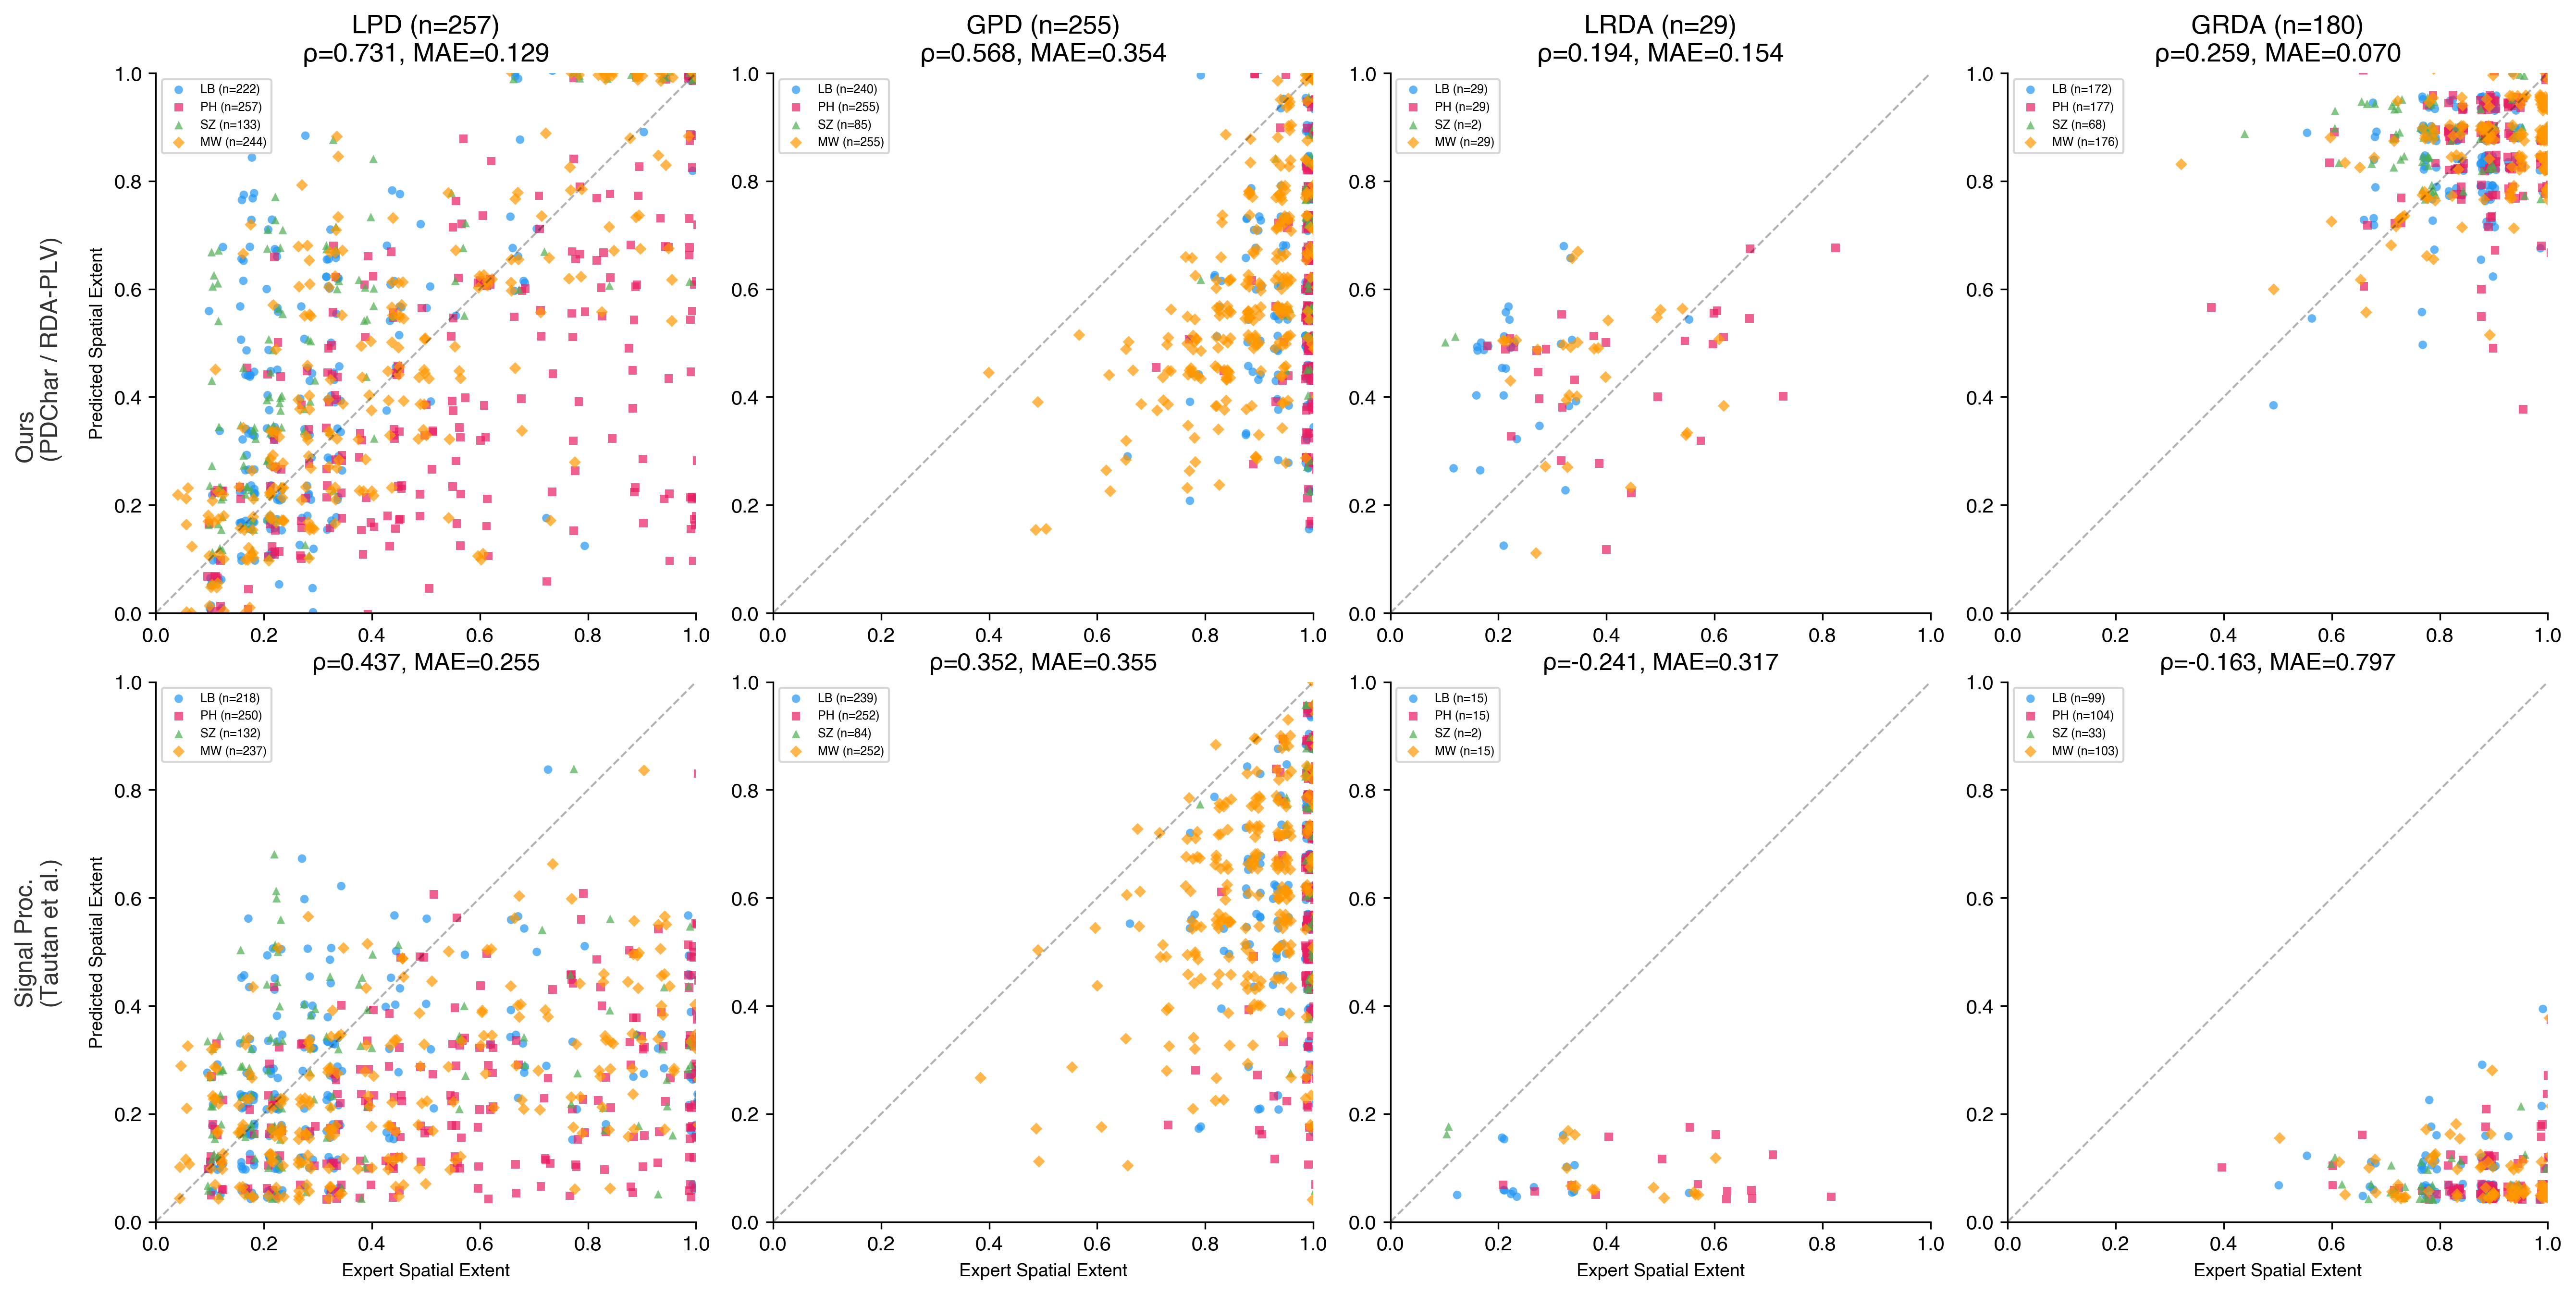
\includegraphics[width=\textwidth]{figures/figS2_spatial_scatter.png}
\caption{Spatial extent scatter plots by subtype. Scatter plots comparing algorithm-predicted spatial extent ($y$-axis, fraction of 18 channels involved) against expert spatial extent ($x$-axis, mean across raters) for each subtype. Per-rater data points shown with distinct markers for each expert rater (LB, PH, SZ, MW). Spearman $\rho$ and MAE are reported per panel.}
\label{fig:spatial_scatter}
\end{figure}

\begin{figure}[htbp]
\centering
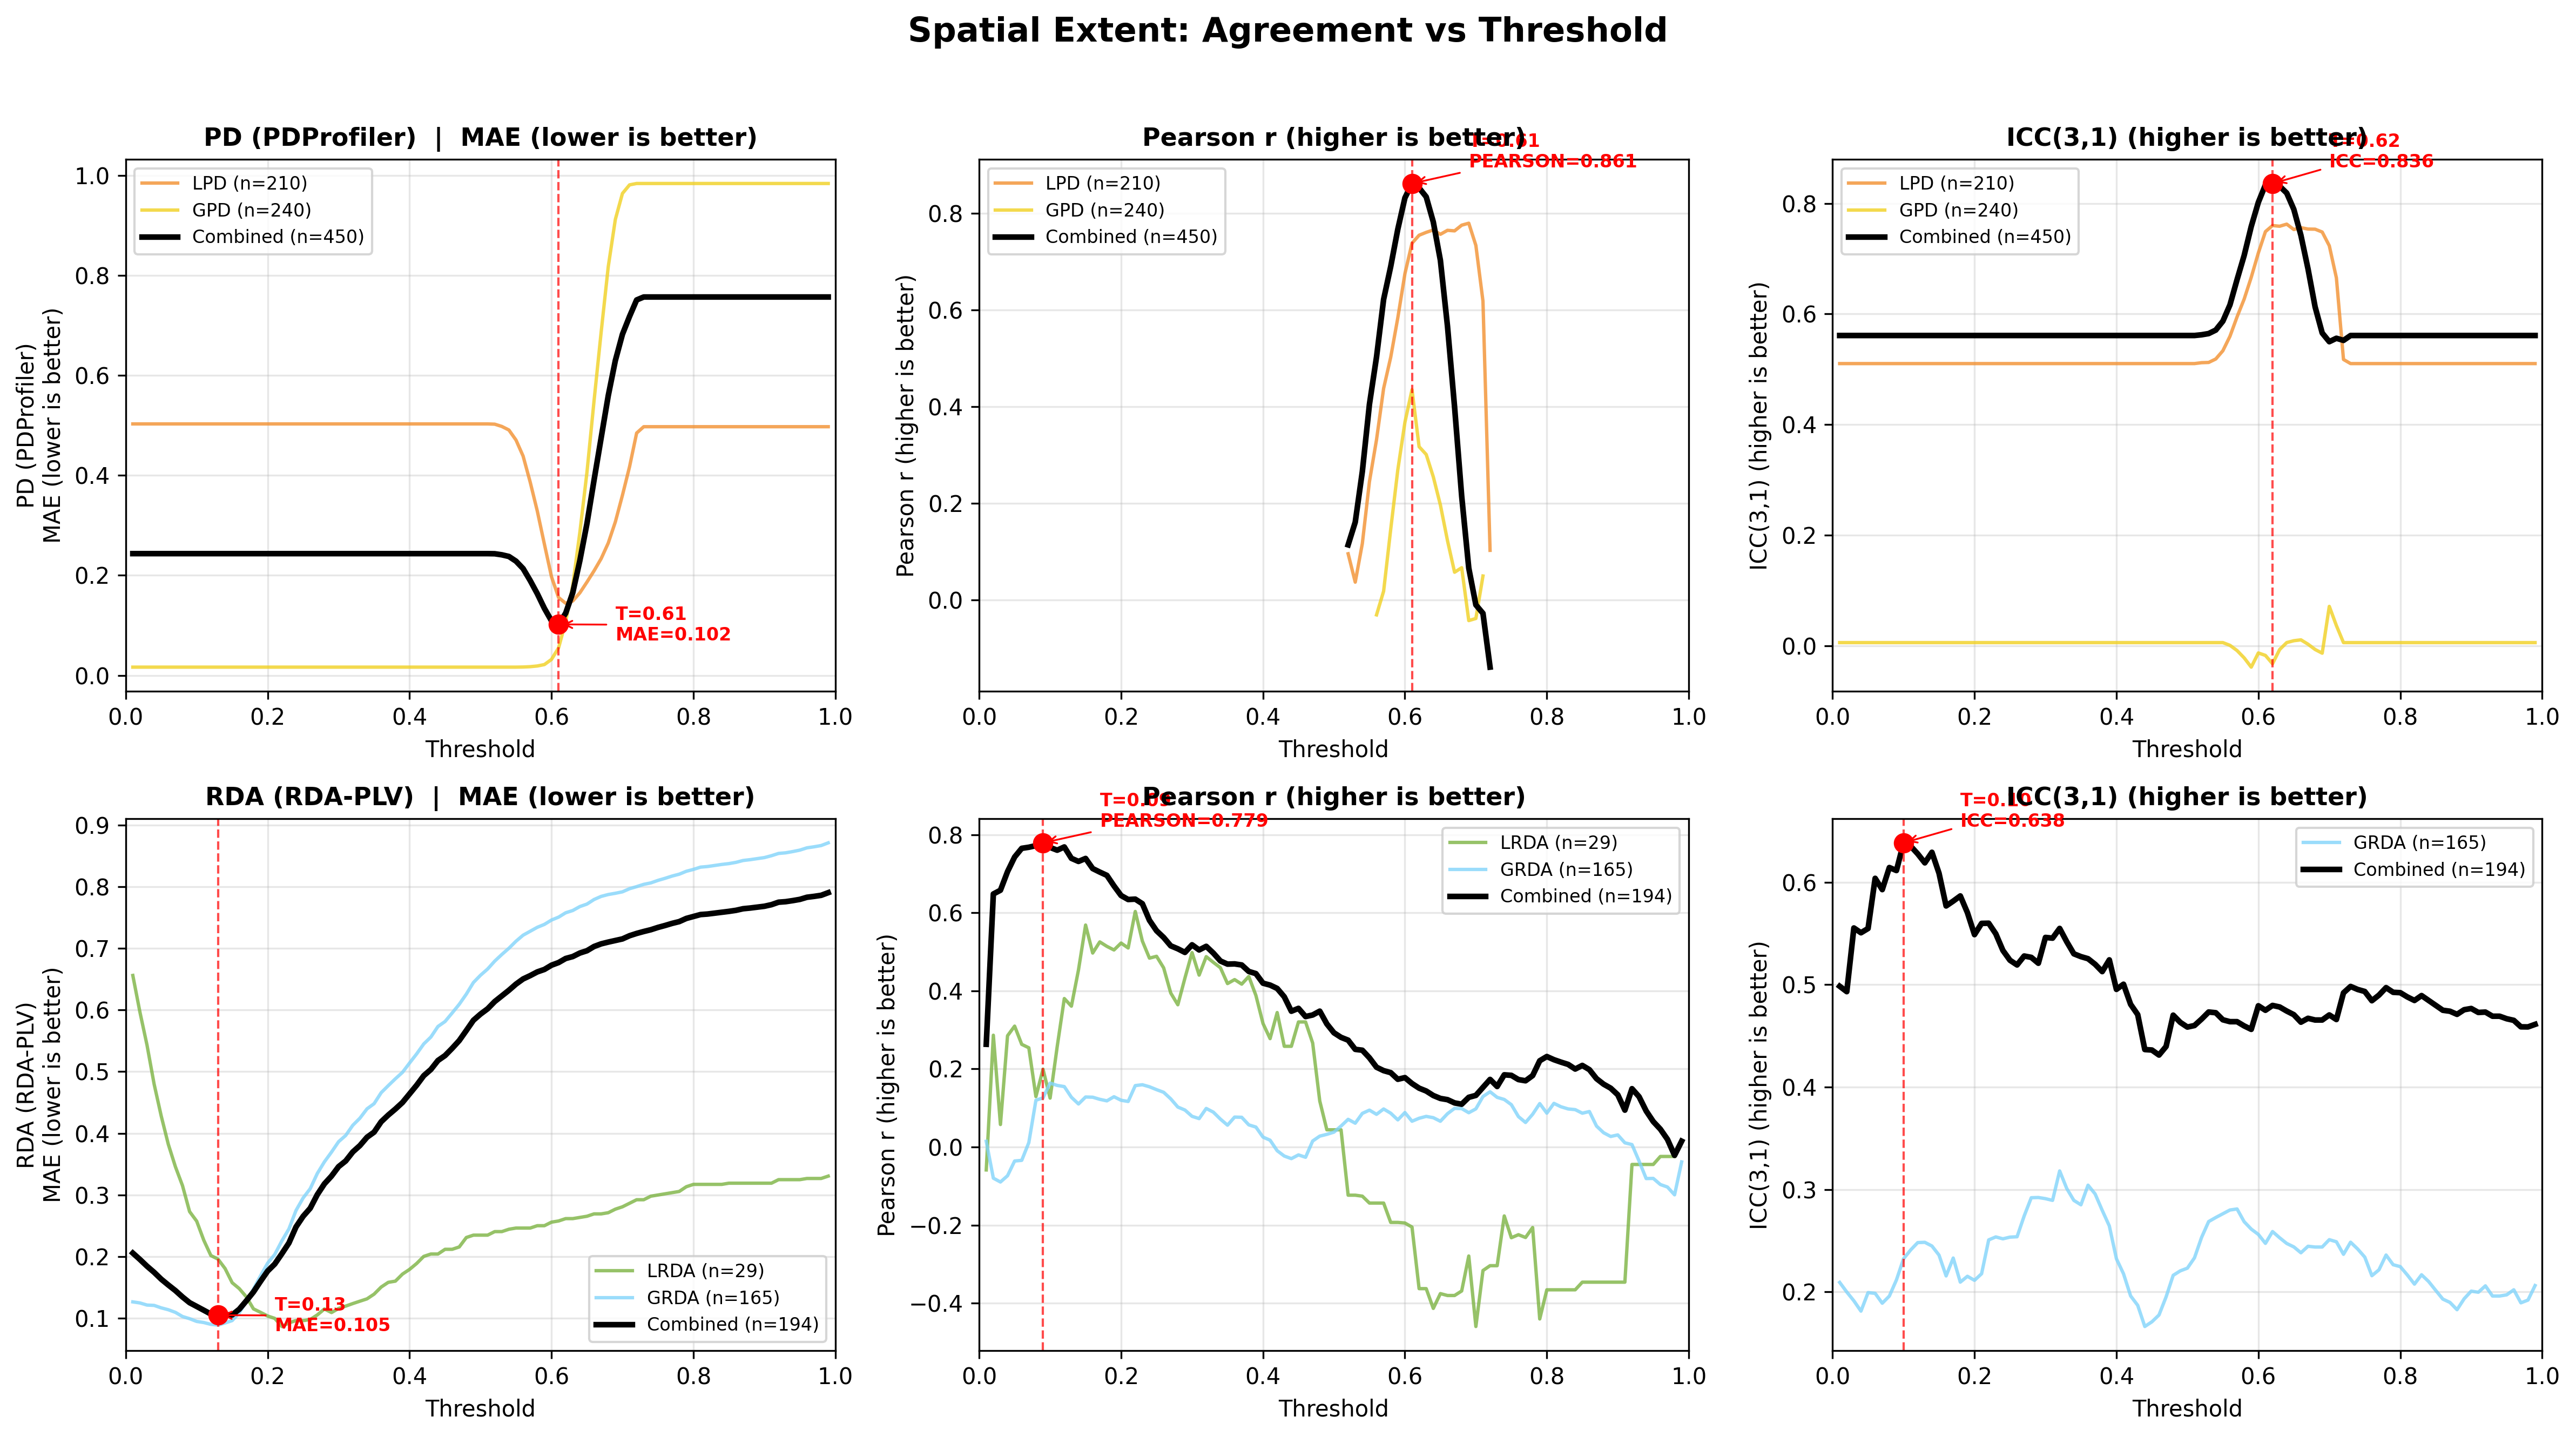
\includegraphics[width=\textwidth]{figures/figS3_threshold_sweep.png}
\caption{Spatial extent threshold optimization. Effect of binarization threshold on spatial extent prediction accuracy, evaluated on segments with at least 2 expert raters. Top row: PD (LPD + GPD). Bottom row: RDA (LRDA + GRDA). Three metrics shown across threshold values (0.01--0.99): MAE, Pearson correlation, and ICC(3,1). Optimal thresholds are marked: PD approximately 0.38--0.62 (broad plateau), RDA approximately 0.15.}
\label{fig:threshold_sweep}
\end{figure}

\begin{figure}[htbp]
\centering
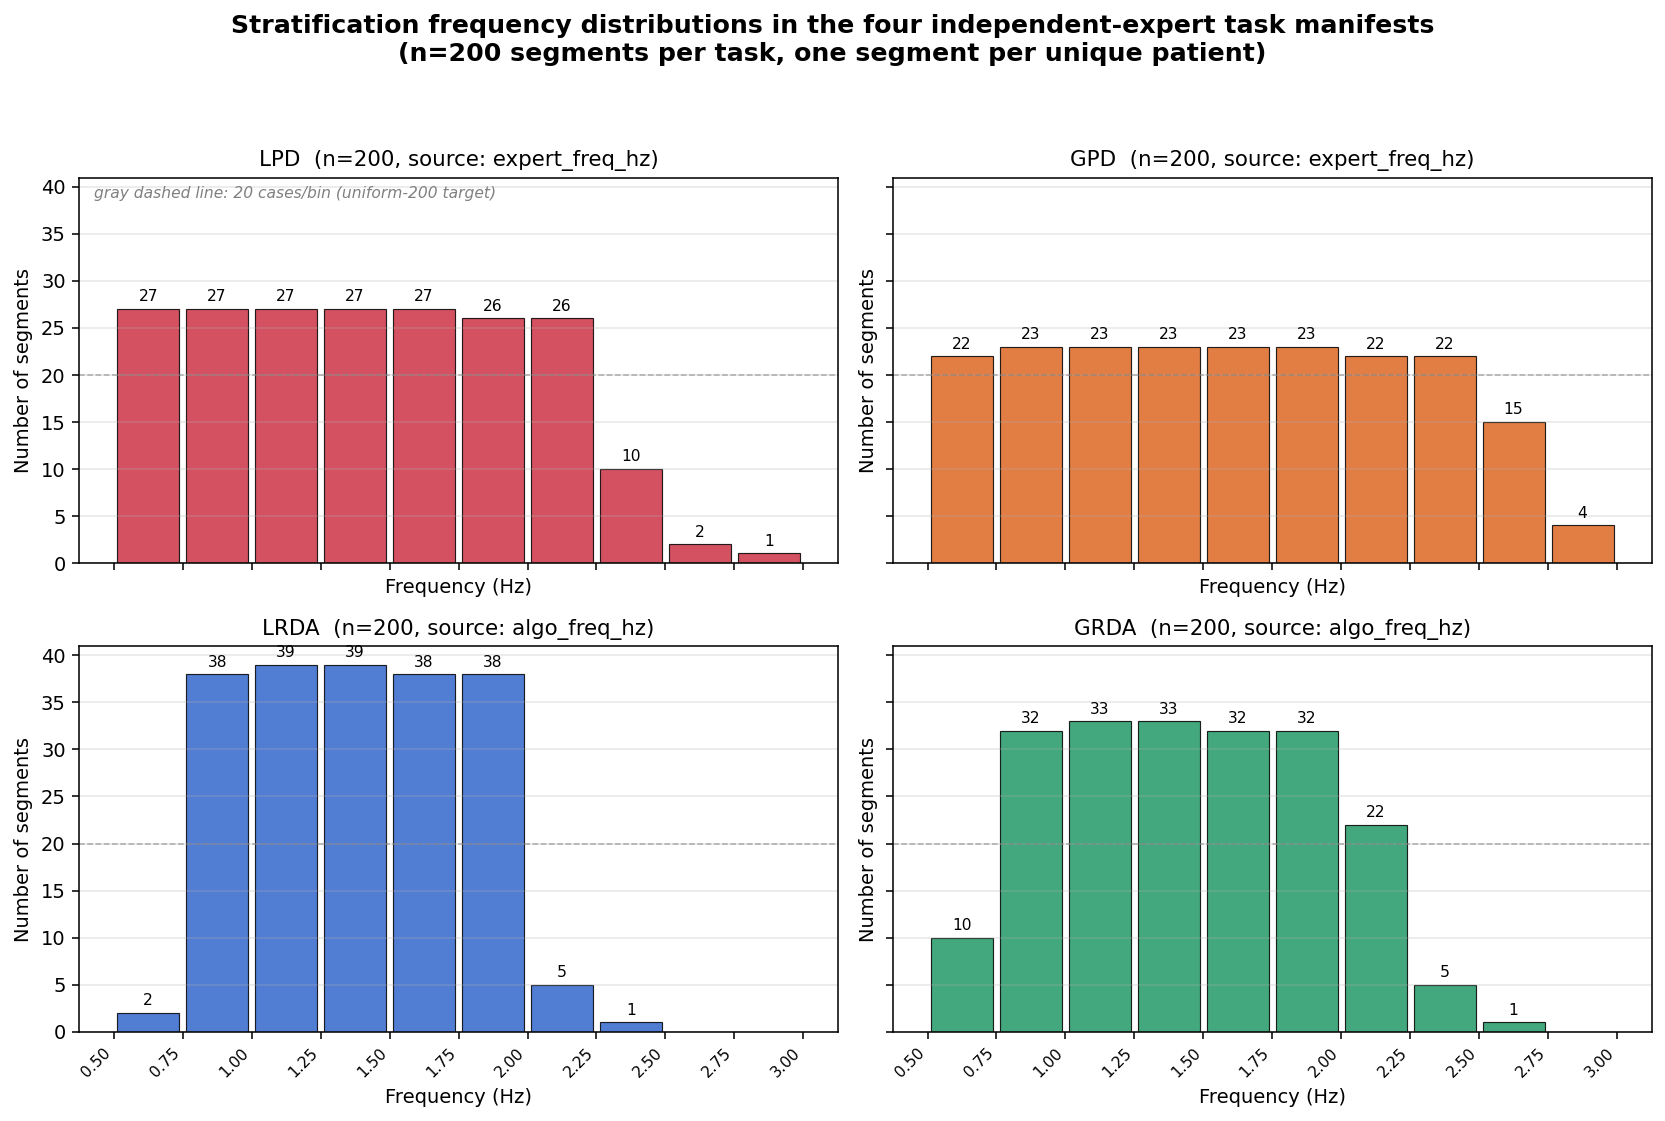
\includegraphics[width=\textwidth]{figures/figS4_independent_expert_freq_distribution.png}
\caption{Stratification frequency distributions for the four independent-expert annotation tasks. Each task contains $n=200$ ten-second EEG segments, one per unique patient, sampled to give approximately uniform coverage of the 0.5--3.0~Hz repetition-frequency range. Bins are 0.25~Hz wide. The gray dashed line at 20 segments/bin indicates the perfectly-uniform-200 target. PD bins (LPD, GPD) are computed from MW's \texttt{expert\_freq\_hz} column, the only PD-frequency column populated in \texttt{segment\_labels.csv}; RDA bins (LRDA, GRDA) are computed from \texttt{algo\_freq\_hz} produced by the RDA-Profiler, independent of any MW labels. The bin assignment is used only to balance coverage; the per-segment default that the new raters see at run time is computed by the PDProfiler / RDA-Profiler at run time, so the new raters never see MW's labels. PDs achieve close-to-uniform distribution across the 0.5--2.25~Hz range; LRDA segments are biology-limited (essentially absent above 2.0~Hz in the dataset) and the stratifier therefore concentrates its 200-segment budget in the populated 0.75--2.0~Hz region. This figure documents the case selection used for the planned independent-rater validation analysis (see \S\ref{sec:limitations} reviewer notes \#1 and \#2).}
\label{fig:indep_expert_freq}
\end{figure}

%%%%%%%%%%%%%%%%%%%%%%%%%%%%%%%%%%%%%%%%%%%%%%%%%%
%% Back matter

\ack{The authors thank the expert electroencephalographers who annotated frequency, discharge timing, and spatial extent for the segments used in this study.}

\funding{Dr.~Westover's laboratory is supported by grants from the National Institutes of Health (R01AG073410, R01HL161253, R01NS126282, R01AG073598, R01NS131347, R01NS130119) and by Amazon Web Services (AWS).}

\section*{Conflict of interest}
Dr.~Westover is a co-founder of, serves as a scientific advisor and consultant to, and has a personal equity interest in Beacon Biosignals. The remaining authors declare no competing interests.

\data{The data that support the findings of this study are available at \url{https://bdsp.io}.}

\roles{%
Jin~Jing: Conceptualization, Methodology, Software, Data Curation, Writing -- Review \& Editing.
ChenXi~Sun: Methodology, Software, Formal Analysis, Writing -- Review \& Editing.
Tianyu~Zhang: Software, Formal Analysis, Writing -- Review \& Editing.
Matthew~Byrd: Software, Formal Analysis, Writing -- Review \& Editing.
Alexandra-Maria~T\u{a}u\c{t}an: Methodology, Software, Data Curation, Writing -- Review \& Editing.
Lara~Basovic: Investigation, Data Curation (annotation), Writing -- Review \& Editing.
Peter~N~Hadar: Investigation, Data Curation (annotation), Writing -- Review \& Editing.
Marta~P~Fernandes: Investigation, Writing -- Review \& Editing.
Daniel~Goldenholz: Investigation, Writing -- Review \& Editing.
Jennifer~Kim: Investigation, Writing -- Review \& Editing.
Aaron~F~Struck: Investigation, Writing -- Review \& Editing.
Sahar~F~Zafar: Investigation, Data Curation (annotation), Writing -- Review \& Editing, Supervision.
M~Brandon~Westover: Conceptualization, Methodology, Software, Validation, Formal Analysis, Investigation, Data Curation, Writing -- Original Draft, Writing -- Review \& Editing, Supervision, Project Administration, Funding Acquisition.%
}

%%%%%%%%%%%%%%%%%%%%%%%%%%%%%%%%%%%%%%%%%%%%%%%%%%
\section*{References}

\begin{thebibliography}{99}

\bibitem{claassen2004}
Claassen J, Mayer SA, Kowalski RG, Emerson RG, Hirsch LJ.
Detection of electrographic seizures with continuous EEG monitoring in critically ill patients.
\textit{Neurology}. 2004;62(10):1743--1748.

\bibitem{chong2005}
Chong DJ, Hirsch LJ.
Which EEG patterns warrant treatment in the critically ill? Reviewing the evidence for treatment of periodic epileptiform discharges and related patterns.
\textit{J Clin Neurophysiol}. 2005;22(2):79--91.

\bibitem{rodriguez2017}
Rodriguez Ruiz A, Vlachy J, Lee JW, et al.
Association of periodic and rhythmic electroencephalographic patterns with seizures in critically ill patients.
\textit{JAMA Neurol}. 2017;74(2):181--188.

\bibitem{hirsch2021}
Hirsch LJ, Fong MWK, Leitinger M, et al.
American Clinical Neurophysiology Society's standardized critical care EEG terminology: 2021 version.
\textit{J Clin Neurophysiol}. 2021;38(1):1--29.

\bibitem{gaspard2014}
Gaspard N, Hirsch LJ, LaRoche SM, Hahn CD, Westover MB; Critical Care EEG Monitoring Research Consortium.
Interrater agreement for critical care EEG terminology.
\textit{Epilepsia}. 2014;55(9):1366--1373.

\bibitem{leitinger2015}
Leitinger M, Beniczky S, Rohracher A, et al.
Salzburg consensus criteria for non-convulsive status epilepticus -- revisited: a critical reappraisal.
\textit{Epilepsy Behav}. 2015;49:158--163.

\bibitem{zafar2020}
Zafar SF, Subramaniam T, Osman G, Herlopian A, Struck AF.
Electrographic seizures and ictal--interictal continuum (IIC) patterns in critically ill patients.
\textit{Epilepsy Behav}. 2020;106:107037. doi:10.1016/j.yebeh.2020.107037.

\bibitem{vespa2016}
Vespa P, Tubi M, Claassen J, Buitrago-Blanco M, McArthur D, Velazquez AG, Tu B, Prins M, Nuwer M.
Metabolic crisis occurs with seizures and periodic discharges after brain trauma.
\textit{Ann Neurol}. 2016;79(4):579--590. doi:10.1002/ana.24606.

\bibitem{struck2016}
Struck AF, Westover MB, Hall LT, Deck GM, Cole AJ, Rosenthal ES.
Metabolic correlates of the ictal--interictal continuum: FDG-PET during continuous EEG.
\textit{Neurocrit Care}. 2016;24(3):324--331. doi:10.1007/s12028-016-0245-y.

\bibitem{tao2020}
Tao JX, Qin X, Wang Q.
Ictal--interictal continuum: a review of recent advancements.
\textit{Acta Epileptol}. 2020;2:13. doi:10.1186/s42494-020-00021-1.

\bibitem{parikh2023}
Parikh H, Hoffman K, Sun H, Zafar SF, Ge W, Jing J, Liu L, Sun J, Struck AF, Volfovsky A, Rudin C, Westover MB.
Effects of epileptiform activity on discharge outcome in critically ill patients in the USA: a retrospective cross-sectional study.
\textit{Lancet Digit Health}. 2023;5(8):e495--e502. doi:10.1016/S2589-7500(23)00088-2.

\bibitem{zafar2021}
Zafar SF, Rosenthal ES, Jing J, Ge W, Tabaeizadeh M, Aboul Nour H, Shoukat M, Sun H, Javed F, Kassa S, Edhi M, Bordbar E, Gallagher J, Moura Junior V, Ghanta M, Shao Y-P, An S, Sun J, Cole AJ, Westover MB.
Automated annotation of epileptiform burden and its association with outcomes.
\textit{Ann Neurol}. 2021;90(2):300--311. doi:10.1002/ana.26161.

\bibitem{gaspard2013}
Gaspard N, Manganas L, Rampal N, Petroff OAC, Hirsch LJ.
Similarity of lateralized rhythmic delta activity to periodic lateralized epileptiform discharges in critically ill patients.
\textit{JAMA Neurol}. 2013;70(10):1288--1295. doi:10.1001/jamaneurol.2013.3475.

\bibitem{furbass2015}
F\"urbass F, Hartmann MM, Halford JJ, Koren J, Herta J, Gruber A, Baumgartner C, Kluge T.
Automatic detection of rhythmic and periodic patterns in critical care EEG based on American Clinical Neurophysiology Society (ACNS) standardized terminology.
\textit{Neurophysiol Clin}. 2015;45(3):203--213. doi:10.1016/j.neucli.2015.08.001.

\bibitem{herta2015}
Herta J, Koren J, F\"urbass F, Hartmann M, Kluge T, Baumgartner C, Gruber A.
Prospective assessment and validation of rhythmic and periodic pattern detection in NeuroTrend: a new approach for screening continuous EEG in the intensive care unit.
\textit{Epilepsy Behav}. 2015;49:273--279. doi:10.1016/j.yebeh.2015.04.064.

\bibitem{mcgraw2024}
McGraw CM, Rao S, Manjunath S, Jing J, Westover MB.
Automated quantification of periodic discharges in human electroencephalogram.
\textit{Biomed Phys Eng Express}. 2024;10(6):065003. doi:10.1088/2057-1976/ad7165.

\bibitem{jing2020}
Jing J, Sun H, Kim JA, et al.
Development of expert-level automated detection of epileptiform discharges during electroencephalogram interpretation.
\textit{JAMA Neurol}. 2020;77(1):103--108. doi:10.1001/jamaneurol.2019.3485.

\bibitem{jing2023irr}
Jing J, Ge W, Struck AF, et al.
Inter-rater reliability of expert electroencephalographers identifying seizures and rhythmic and periodic patterns in EEGs.
\textit{Neurology}. 2023;100(17):e1737--e1749. doi:10.1212/WNL.0000000000207003.

\bibitem{gramfort2013}
Gramfort A, Luessi M, Larson E, et al.
MEG and EEG data analysis with MNE-Python.
\textit{Front Neurosci}. 2013;7:267. doi:10.3389/fnins.2013.00267.

\bibitem{shrout1979}
Shrout PE, Fleiss JL.
Intraclass correlations: uses in assessing rater reliability.
\textit{Psychol Bull}. 1979;86(2):420--428. doi:10.1037/0033-2909.86.2.420.

\bibitem{jing2023}
Jing J, Ge W, Hong S, et al.
Development of expert-level classification of seizures and rhythmic and periodic patterns during EEG interpretation.
\textit{Neurology}. 2023;100(17):e1750--e1762.

\bibitem{ge2023}
Ge W, Jing J, An S, et al.
Deep active learning for interictal ictal injury continuum EEG patterns.
\textit{J Neurosci Methods}. 2023;390:109835.

\bibitem{zheng2022}
Zheng WL, Amorim E, Jing J, et al.
Predicting neurological outcome from electroencephalogram dynamics in comatose patients after cardiac arrest with deep learning.
\textit{IEEE Trans Biomed Eng}. 2022;69(5):1813--1825.

\bibitem{tautan2025}
T\u{a}u\c{t}an AM, Jing J, Basovic L, Hadar PN, Sartipi S, Fernandes MP, Kim J, Struck AF, Westover MB, Zafar SF.
Automated estimation of frequency and spatial extent of periodic and rhythmic epileptiform activity from continuous electroencephalography data.
\textit{J Neural Eng}. 2025;22(6):066027. doi:10.1088/1741-2552/ae2716.

\bibitem{lake2017}
Lake BM, Ullman TD, Tenenbaum JB, Gershman SJ.
Building machines that learn and think like people.
\textit{Behav Brain Sci}. 2017;40:e253.

\end{thebibliography}

\end{document}
